\documentclass[a4paper,11pt,]{book} % draft

\usepackage{silence}
\WarningFilter{fourier}{Please consider}
\WarningFilter{hyperref}{Token not allowed in a PDF string}

\usepackage[T1]{fontenc}
\usepackage{fontspec}
\usepackage[french,english]{babel}
\setmonofont{Ubuntu Mono}
\setlength{\textwidth}{146.8mm}
\setlength{\oddsidemargin}{11.6mm}
\setlength{\evensidemargin}{0.8mm}
\setlength{\topmargin}{-2.2mm}
\setlength{\textheight}{221.9mm}
\setlength{\headheight}{14pt}

\usepackage{setspace}
\setstretch{1.1}
\makeatletter
\setlength{\@fptop}{0pt}
\makeatother

\usepackage{lmodern}
\usepackage{fourier}
\usepackage{graphicx}
\usepackage{xcolor}
\usepackage{booktabs}
\usepackage{lipsum}
\usepackage[final]{microtype}
\usepackage[hyphens]{url}

\usepackage{fancyhdr}
\renewcommand{\sectionmark}[1]{\markright{\thesection\ #1}}
\pagestyle{fancy}
  \fancyhf{}
  \renewcommand{\headrulewidth}{0.4pt}
  \renewcommand{\footrulewidth}{0pt}
  \fancyhead[OR]{\bfseries \nouppercase{\rightmark}}
  \fancyhead[EL]{\bfseries \nouppercase{\leftmark}}
  \fancyfoot[EL,OR]{\thepage}
\fancypagestyle{plain}{
  \fancyhf{}
  \renewcommand{\headrulewidth}{0pt}
  \renewcommand{\footrulewidth}{0pt}
  \fancyfoot[EL,OR]{\thepage}}
\fancypagestyle{addpagenumbersforpdfimports}{
  \fancyhead{}
  \renewcommand{\headrulewidth}{0pt}
  \fancyfoot{}
  \fancyfoot[RO,LE]{\thepage}
}

\usepackage[final]{hyperref}
\definecolor[named]{purplish}{cmyk}{0.55,1,0,0.15}
\definecolor[named]{darkblueish}{cmyk}{1,0.58,0,0.21}
\hypersetup{
  colorlinks=true,
  pdfborder={0 0 0},
  linkcolor=purplish,
  citecolor=purplish,
  urlcolor=darkblueish,
  filecolor=darkblueish}
\urlstyle{same}
\usepackage[final]{pdfpages}
\usepackage{bookmark}

\makeatletter
\renewcommand\@pnumwidth{20pt}
\makeatother

\makeatletter
\def\cleardoublepage{\clearpage\if@twoside \ifodd\c@page\else
    \hbox{}
    \thispagestyle{empty}
    \newpage
    \if@twocolumn\hbox{}\newpage\fi\fi\fi}
\makeatother \clearpage{\pagestyle{plain}\cleardoublepage}

\usepackage{color}
\usepackage{tikz}
\usepackage[explicit]{titlesec}
\newcommand*\chapterlabel{}
\titleformat{\chapter}[display]
  {\normalfont\bfseries\Huge}
  {\gdef\chapterlabel{\thechapter\ }}
  {0pt}
    {\begin{tikzpicture}[remember picture,overlay]
    \node[yshift=-8cm] at (current page.north west)
      {\begin{tikzpicture}[remember picture, overlay]
        \draw[fill=black] (0,0) rectangle(35.5mm,15mm);
        \node[anchor=north east,yshift=-7.2cm,xshift=34mm,minimum height=30mm,inner sep=0mm] at (current page.north west)
        {\parbox[top][30mm][t]{15mm}{\raggedleft \rule{0cm}{0.6cm}\color{white}\chapterlabel}};  %the empty rule is just to get better base-line alignment
        \node[anchor=north west,yshift=-7.2cm,xshift=37mm,text width=\textwidth,minimum height=30mm,inner sep=0mm] at (current page.north west)
              {\parbox[top][30mm][t]{\textwidth}{\rule{0cm}{0.6cm}\color{black}#1}};
       \end{tikzpicture}
      };
   \end{tikzpicture}
   \gdef\chapterlabel{}
  } % code before the title body
\titlespacing*{name=\chapter,numberless}{-3.7cm}{83.2pt-\parskip}{-3.2pt+\parskip}
\titlespacing*{\chapter}{-3.7cm}{50pt-\parskip-\parskip}{30pt+\parskip+\parskip}
\titlespacing*{\section}{0pt}{13.2pt}{1em-\parskip}  % 13.2pt is line spacing for a text with 11pt font size
\titlespacing*{\subsection}{0pt}{13.2pt}{1em-\parskip}
\titlespacing*{\subsubsection}{0pt}{13.2pt}{1em-\parskip}
\titlespacing*{\paragraph}{0pt}{13.2pt}{1em-\parskip}

\newcounter{myparts}
\newcommand*\partlabel{}
\titleformat{\part}[display]  % type (section,chapter,etc...) to vary,  shape (eg display-type)
  {\normalfont\bfseries\Huge} % format of the part
  {\gdef\partlabel{\thepart\ }}     % the label
  {0pt} % separation between label and part-title
    {\ifpdf\setlength{\unitlength}{20mm}\else\setlength{\unitlength}{0mm}\fi
    \addtocounter{myparts}{1}
    \begin{tikzpicture}[remember picture,overlay]
    \node[anchor=north west,xshift=-65mm,yshift=-6.9cm-\value{myparts}*20mm] at (current page.north east) % for unknown reasons: 3mm missing -> 65 instead of 62
      {\begin{tikzpicture}[remember picture, overlay]
        \draw[fill=black] (0,0) rectangle(62mm,20mm);   % -\value{myparts}\unitlength
        \node[anchor=north west,yshift=-6.1cm-\value{myparts}*\unitlength,xshift=-60.5mm,minimum height=30mm,inner sep=0mm] at (current page.north east)
        {\parbox[top][30mm][t]{55mm}{\raggedright \color{white}Part \partlabel \rule{0cm}{0.6cm}}};  %the empty rule is just to get better base-line alignment
        \node[anchor=north east,yshift=-6.1cm-\value{myparts}*\unitlength,xshift=-63.5mm,text width=\textwidth,minimum height=30mm,inner sep=0mm] at (current page.north east)
              {\parbox[top][30mm][t]{\textwidth}{\raggedleft \rule{0cm}{0.6cm}\color{black}#1}};
       \end{tikzpicture}
      };
   \end{tikzpicture}
   \gdef\partlabel{}
  } % code before the title body
\titlespacing*{\part}{11.06cm}{26.4pt-\parskip-\parskip}{0pt}

\usepackage{amsmath}
\usepackage{amsfonts}
\usepackage{amssymb}
\usepackage{mathtools}
\usepackage{xstring}
% Fix the problem with delimiter size caused by fourier and amsmath packages.
\makeatletter
\def\resetMathstrut@{%
  \setbox\z@\hbox{%
    \mathchardef\@tempa\mathcode`\(\relax
      \def\@tempb##1"##2##3{\the\textfont"##3\char"}%
      \expandafter\@tempb\meaning\@tempa \relax
  }%
  \ht\Mathstrutbox@1.2\ht\z@ \dp\Mathstrutbox@1.2\dp\z@
}
\makeatother


%%%%%%%%%%%%%%%%%%%%%%%%%%%%%%%%%%%%%%%%%%%%%%%%%%
%%%%%%%%%%%% Match Type paper headers %%%%%%%%%%%%
%%%%%%%%%%%%%%%%%%%%%%%%%%%%%%%%%%%%%%%%%%%%%%%%%%

\usepackage{amsthm}
\usepackage[nameinlink]{cleveref}
\usepackage[final]{listings}
\usepackage{bcprules}
\usepackage{proof}
\usepackage{framed}
\usepackage{xspace}
\usepackage{mdframed}
\usepackage[square]{natbib}

\crefname{subsection}{subsection}{subsections}

% Label examples as Example A, B, C, ...
% https://tex.stackexchange.com/a/195979/31377
% https://tex.stackexchange.com/a/118285/31377
\newcounter{example}[section]
\newenvironment{example}[1][]{\refstepcounter{example}\par\medskip%
\textbf{Example~\symbol{\numexpr64+\theexample}. #1} \rmfamily}{\medskip}
\creflabelformat{example}{#2\symbol{\numexpr64+#1}#3}

\lstdefinelanguage{scala}{
  alsoletter={@,=,>},
  morekeywords={
    abstract, case, class, def, else, extends, false, if, implicit,
    match, object, true, val, var, while, sealed, for, dependent, null, type,
    with, try, catch, finally, import, final, return, new, override, this,
    trait, private, public, protected, package, throw, enum,
    newtype % laziness at it's best
  },
  sensitive=true,
  morecomment=[l]{//},
  morecomment=[s]{/*}{*/},
  morestring=[b]"
}
\lstset{
  language=scala,
  basicstyle=\ttfamily\small,
  keepspaces=true,
  showstringspaces=false,
  columns=fullflexible,
  escapeinside={(*}{*)},
  belowskip=0.5em,aboveskip=0.5em,
  xleftmargin=0pt,
  xrightmargin=0pt
}

\lstdefinestyle{py}{language=Python, otherkeywords={as}}
\lstdefinestyle{scala}{language=scala}
\lstdefinestyle{typescript}{language=scala, otherkeywords={function}}

\usepackage[autostyle=false, style=english]{csquotes}
\MakeOuterQuote{"}

% Hide proofs
\usepackage{environ}
\NewEnviron{killcontents}{}
\let\proof\killcontents
\let\endproof\endkillcontents

\newcommand\lbl[1]{%
  \ifcsname c@#1\endcsname%
  \addcontentsline{toc}{section}{\Cref*{#1}:~\nameref{#1}}%
  \else\newcounter{#1}\label{#1}%
  \fi%
}
\newcommand{\mathkw}[1]{\text{\itshape#1}}

\def\({(}
\def\+{+}
\def\-{-}
\def\3{3}
\def\4{4}
\def\:{\operatorname{:}\allowbreak}
\def\<:{\allowbreak\operatorname{\normalfont\text{<}:}\allowbreak}
\def\={=\allowbreak}
\def\[{[}
\def\andalso{\;\quad}
\def\Any{\normalfont\text{Any}}
\def\A{\normalfont\text{A}}
\def\a{\normalfont\text{a}}
\def\bind{\normalfont\text{bind}}
\def\Bur{\normalfont\text{Bar}}
\def\bur{\normalfont\text{bar}}
\def\Buzz{\normalfont\text{Buzz}}
\def\buzz{\normalfont\text{buzz}}
\def\B{\normalfont\text{B}}
\def\b{\normalfont\text{b}}
\def\Case{\item\textit{Case~}}
\def\case{\mathkw{case}}
\def\c{\normalfont\text{c}}
\def\C{\normalfont\text{C}}
\def\DXi{\textsc{D-Xi}\xspace}
\def\DPsi{\textsc{D-Psi}\xspace}
\def\DAll{\textsc{D-All}\xspace}
\def\DArrow{\textsc{D-Arrow}\xspace}
\def\disj{\normalfont\text{disj}}
\def\DSub{\textsc{D-Sub}\xspace}
\def\d{\normalfont\text{d}}
\def\EAppAbs{\textsc{E-AppAbs}\xspace}
\def\EAppA{\textsc{E-App1}\xspace}
\def\EAppB{\textsc{E-App2}\xspace}
\def\EMatch#1{\textsc{E-Match#1}\xspace}
\def\BEMatch#1{\textsc{BE-Match#1}\xspace}
\def\ETAppTAbs{\textsc{E-TAppTAbs}\xspace}
\def\ETApp{\textsc{E-TApp}\xspace}
\def\e{\normalfont\text{e}}
\def\E{\normalfont\text{E}}
\def\false{\normalfont\text{false}}
\def\Fm{\normalfont{FM}\xspace}
\def\FmB{\normalfont{FMB}\xspace}
\def\Foo{\normalfont\text{Foo}}
\def\foo{\normalfont\text{foo}}
\def\Fsub{\normalfont{F}\ensuremath{_{\<:}}\xspace}
\def\f{\normalfont\text{f}}
\def\F{\normalfont\text{F}}
\def\G{\normalfont\text{G}}
\def\iff{\normalfont\text{iff}}
\def\k{\normalfont\text{k}}
\def\match{~\mathkw{match}}
\def\Match{~\normalfont\text{Match}}
\def\M{\normalfont\text{M}}
\def\m{m}
\def\new{\mathkw{new}~}
\def\Nothing{\normalfont\text{Nothing}}
\def\n{n}
\def\otherwise{\mathkw{or}~}
\def\P{\normalfont\text{P}}
\def\q{\normalfont\text{q}}
\def\Q{\normalfont\text{Q}}
\def\SAll{\textsc{S-All}\xspace}
\def\SCons{\texttt{\#:}\xspace}
\def\SArrow{\textsc{S-Arrow}\xspace}
\def\Shape{\texttt{Shape}\xspace}
\def\SPsi{\textsc{S-Psi}\xspace}
\def\SMatch#1{\textsc{S-Match#1}\xspace}
\def\BSMatch#1{\textsc{BS-Match#1}\xspace}
\def\SNil{\texttt{SNil}\xspace}
\def\SRefl{\textsc{S-Refl}\xspace}
\def\STop{\textsc{S-Top}\xspace}
\def\STrans{\textsc{S-Trans}\xspace}
\def\SSin{\textsc{S-Sin}\xspace}
\def\STvar{\textsc{S-TVar}\xspace}
\def\Subcase{\item\textit{Subcase~}}
\def\Subsubcase{\item\textit{Subsubcase~}}
\def\SystemFm{System~\Fm}
\def\SystemFmB{System~\FmB}
\def\SystemFsub{System~\Fsub}
\def\s{\normalfont\text{s}}
\def\S{\normalfont\text{S}}
\def\TAbs{\textsc{T-Abs}\xspace}
\def\TApp{\textsc{T-App}\xspace}
\def\TClass{\textsc{T-Class}\xspace}
\def\TMatch{\textsc{T-Match}\xspace}
\def\BTMatch{\textsc{BT-Match}\xspace}
\def\Top{\normalfont\text{Top}}
\def\true{\normalfont\text{true}}
\def\TSub{\textsc{T-Sub}\xspace}
\def\TTAbs{\textsc{T-TAbs}\xspace}
\def\TTApp{\textsc{T-TApp}\xspace}
\def\TVar{\textsc{T-Var}\xspace}
\def\T{\normalfont\text{T}}
\def\t{\normalfont\text{t}}
\def\U{\normalfont\text{U}}
\def\u{\normalfont\text{u}}
\def\V{\normalfont\text{V}}
\def\v{\normalfont\text{v}}
\def\W{\normalfont\text{W}}
\def\x{\normalfont\text{x}}
\def\xs{\normalfont\text{xs}}
\def\X{\normalfont\text{X}}
\def\y{\normalfont\text{y}}
\def\Y{\normalfont\text{Y}}
\def\·{\cdot}
\def\×{\times}
\def\Γ{\Gamma}
\def\Δ{\Delta}
\def\Λ{\Lambda}
\def\λ{\lambda}
\def\Ψ{\Psi}
\def\ℕ{\mathbb{N}}
\def\Ξ{\Xi}
\def\→{\operatorname{\rightarrow}\allowbreak}
\def\↦{\operatorname{\mapsto}\allowbreak}
\def\⇌{\operatorname{\rightleftharpoons}\allowbreak}
\def\⇒{\operatorname{\Rightarrow}\allowbreak}
\def\∀{\forall}
\def\∃{\exists}
\def\∄{\nexists}
\def\∈{\operatorname{\in}\allowbreak}
\def\∉{\operatorname{\notin}\allowbreak}
\def\∩{\operatorname{\cap}\allowbreak}
\def\∪{\operatorname{\cup}\allowbreak}
\def\≠{\operatorname{\neq}\allowbreak}
\def\≡{\allowbreak\operatorname{\normalfont\text{=}:\!\normalfont\text{=}}\allowbreak}
\def\⊂{\operatorname{\subset}\allowbreak}
\def\⊢{\allowbreak\operatorname{\vdash}\allowbreak}
\def\⟦{\llbracket}
\def\⟧{\rrbracket}
\def\|{|}
\def\⟶{\operatorname{\longrightarrow}\allowbreak}
\def\Ø{\emptyset}
\def\Char{\normalfont\text{Char}}
\def\List{\normalfont\text{List}}
\def\Seq{\normalfont\text{Seq}}
\def\String{\normalfont\text{String}}
\def\W{\normalfont\text{W}}
\def\D{\normalfont\text{D}}
\def\R{\normalfont\text{R}}
\def\H{\normalfont\text{H}}
\def\Z{\normalfont\text{Z}}
\def\List{\normalfont\text{List}}
\def\Int{\normalfont\text{Int}}
\def\Id{\normalfont\text{Id}}

\crefname{lem}{lemma}{lemmas}
\Crefname{lem}{Lemma}{Lemmas}
\crefname{thm}{theorem}{theorems}
\Crefname{thm}{Theorem}{Theorems}
\newcommand\prelemma[1]{%
  \stepcounter{theorem}
  \textbf{\thmname{Lemma}\thmnumber{~\thetheorem}}\thmnote{ (#1)}%
}

\newtheoremstyle{plain}
  {\topsep}    % ABOVESPACE
  {\topsep}    % BELOWSPACE
  {\itshape}   % BODYFONT
  {}           % INDENT
  {\bfseries}  % HEADFONT
  {.}          % HEADPUNCT
  {5pt plus 1pt minus 1pt} % HEADSPACE
  {\thmname{#1}\thmnumber{ \StrSubstitute{#2}{A}{4}}\thmnote{ \normalfont(#3)}}
\theoremstyle{plain}

\newtheorem{theorem}{Theorem}[chapter]
\newtheorem{lemma}[theorem]{Lemma}
\newtheorem*{definition*}{Definition}

\lstMakeShortInline{|}
% Properly spaced highlight
\definecolor{light-gray}{gray}{0.85}
\setlength{\fboxsep}{0pt}%
\newcommand\reducedstrut{\vrule width 0pt height .9\ht\strutbox depth .4\dp\strutbox\relax}
\newcommand\hl[1]{\!\colorbox{light-gray}{\,\ensuremath{\reducedstrut#1}\,}}
\def\nquad{\hspace{-20pt}}

% Highlighted infrule/infax
\def\hlrule[#1]{\maybeindex{#1}\hlrulee{\inflabel{#1}}}
\def\hlrulee#1#2#3{\layoutrule{#1}{\colorbox{light-gray}{\ensuremath{\typesetrule{#2}{#3}}\ignorespaces}}}
\def\hlax[#1]{\maybeindex{#1}\hlaxx{\inflabel{#1}}}
\def\hlaxx#1#2{\layoutrule{#1}{\colorbox{light-gray}{\ensuremath{\reducedstrut{#2}}\ignorespaces}}}

\def\thirdA{\begin{minipage}[t]{0.32\linewidth}}
\def\thirdB{\end{minipage}\begin{minipage}[t]{0.32\linewidth}}
\def\thirdC{\end{minipage}\begin{minipage}[t]{0.32\linewidth}}
\def\thirdD{\end{minipage}\medskip\smallskip}
\def\halfA{\hspace{0.04\linewidth}\begin{minipage}[t]{0.45\linewidth}}
\def\halfB{\end{minipage}\hspace{0.02\linewidth}\begin{minipage}[t]{0.45\linewidth}}
\def\halfC{\end{minipage}\medskip\smallskip}

\newcommand\FMSyntaxEvaluation[1]{
  \begin{figure}%
  \begin{framed}%
  \begin{minipage}[t]{\linewidth}%
    \textit{Syntax}%
  \end{minipage}%

  \begin{minipage}[t]{.40\linewidth}%
    \vspace{-10pt}%
    \hfuzz=50pt
    \begin{flalign*}%
    \t \Coloneqq ~&&
      \\[-3pt] & \x                         & \textit{variable}
      \\[-3pt] & \λ\x \: \T.~ \t             & \textit{abstraction}
      \\[-3pt] & \λ\X \<: \T.~ \t            & \textit{type abstraction}
      \\[-3pt] & \t~\t                      & \textit{application}
      \\[-3pt] & \t~\T                      & \textit{type application}
      \\[-3pt] & \hl{\new \C}               & \textit{constructor call}
      \\[-3pt] & \hl{\t~\match \{ \overline{\x \: \C \⇒ \t} \} \otherwise~\t}
                                     \nquad & \textit{match expr.}
      \\
    \v \Coloneqq ~&&
      \\[-3pt] & \λ\x \: \T.~\t              & \textit{abstraction}
      \\[-3pt] & \λ\X \<: \T.~\t             & \textit{type abstraction}
      \\[-3pt] & \hl{\new \C}               & \textit{constructor call}
    \end{flalign*}%
    \hfuzz=0pt
  \end{minipage}%
  \hfill%
  \vline%
  \hfill%
  \begin{minipage}[t]{.40\linewidth}%
    \vspace{-10pt}%
    \hfuzz=50pt
    \begin{flalign*}%
    \T \Coloneqq ~&&
      \\[-3pt] & \X                         & \textit{type variable}
      \\[-3pt] & \T \rightarrow \T          & \textit{type of functions}
      \\[-3pt] & \forall \X \<: \T.~\T      & \textit{universal type}
      \\[-3pt] & \Top                       & \textit{maximum type}
      \\[-3pt] & \hl{\C}                    & \textit{class}
      \\[-3pt] & \hl{\{ \new \C \}} \nquad  & \textit{constructor singleton}
      \\[-3pt] & \hl{\T~\match \{ \overline{\T \⇒ \T} \} \otherwise~\T}
                                     \nquad & \textit{match type}
      \\
    \Γ \Coloneqq ~&&
      \\[-3pt] & \Ø                         & \textit{empty context}
      \\[-3pt] & \Γ, \x \: \T                & \textit{term binding}
      \\[-3pt] & \Γ, \X \<: \T               & \textit{type binding}
    \end{flalign*}%
    \hfuzz=0pt
  \end{minipage}%
  \end{framed}%
  \medskip
  \begin{framed}%
  \begin{minipage}[t]{\linewidth}%
    \textit{Evaluation}
    \medskip

    \thirdA
    \infrule[E-App1]
      { \t_1 \⟶ \t_1' }
      { \t_1~\t_2 \⟶ \t_1'~\t_2 }
    \thirdB
    \infrule[E-App2]
      { \t_2 \⟶ \t_2' }
      { \v_1~\t_2 \⟶ \v_1~\t_2' }
    \thirdC
    \infrule[E-TApp]
      { \t_1 \⟶ \t_1' }
      { \t_1~\T_2 \⟶ \t_1'~\T_2 }
    \thirdD

    \halfA
    \infax[E-AppAbs]
      { (\λ\x \: \T_{11}.~\t_{12})~\v_2 \⟶ [\x \↦ \v_2]\t_{12} }
    \halfB
    \infax[E-TAppTAbs]
      { (\λ\X \<: \T_{11}.~\t_{12})~\T_2 \⟶ [\X \↦ \T_2]\t_{12}}
    \halfC

    \begin{center}
    \begin{minipage}[T]{0.8\linewidth}
    \hlrule[E-Match1]
      { \t_s \⟶ \t'_s }
      { \,\t_s\match \{ \x_i \: \C_i \⇒ \t_i \} \otherwise~\t_d \⟶\\
         \t'_s\match \{ \x_i \: \C_i \⇒ \t_i \} \otherwise~\t_d \hphantom{\⟶}}
    \bigskip
    \hlrule[E-Match2]
      { (\C, \C_n) \∈ \Ψ  \andalso
        \∀m<n.~(\C, \C_m) \∉ \Ψ}
      { \new \C~\match \{ \x_i \: \C_i \⇒ \t_i\} \otherwise~\t_d \⟶ [\x_n \↦ \new \C]\t_n }
    \bigskip
    \hlrule[E-Match3]
      { \∀m.~(\C, \C_m) \∉ \Ψ }
      { \new \C~\match \{ \x_i \: \C_i \⇒ \t_i\} \otherwise~\t_d \⟶ \t_d }
    \bigskip
    \hlax[E-Match4]
      { \,(\λ\x \: \T.~\t)\match \{ \x_i \: \C_i \⇒ \t_i\} \otherwise~\t_d \⟶ \t_d\, }
    \bigskip
    \hlax[E-Match5]
      { \,(\λ\X \<: \T.~\t)\match \{ \x_i \: \C_i \⇒ \t_i\} \otherwise~\t_d \⟶ \t_d\, }
    \end{minipage}
    \end{center}
  \end{minipage}%
  \end{framed}%
  \captionsetup{justification=centering}%
  \caption{#1}%
  \label{fig:FMSyntaxEvaluation}%
  \end{figure}%
}

\newcommand\FMTypingRules[1]{
  \clearpage%
  \thispagestyle{empty}%
  \begin{figure}%
  \vspace{-25pt}%
  \begin{framed}%
  \begin{minipage}[t]{\linewidth}%
    \textit{Subtyping} %%%%%%%%%%%%%%%%%%%%%%%%%%%%%%%%%%%%%%%%%%%%%%%%%%%%
    \medskip

    \halfA
    \infax[S-Refl]
      { \Γ \⊢ \S \<: \S }
    \halfB
    \infax[S-Top]
      { \Γ \⊢ \S \<: \Top }
    \halfC

    \halfA
    \hlax[S-Sin]
      { \,\Γ \⊢ \{ \new \C \} \<: \C\, }
    \halfB
    \hlrule[S-Psi]
      { (\C_1, \C_2) \∈ \Ψ }
      { \Γ \⊢ \C_1 \<: \C_2 }
    \halfC

    \halfA
    \infrule[S-Trans]
      { \Γ \⊢ \S \<: \U  \andalso  \Γ \⊢ \U \<: \T }
      { \Γ \⊢ \S \<: \T }
    \halfB
    \infrule[S-Arrow]
      { \Γ \⊢ \T_1 \<: \S_1  \andalso  \Γ \⊢ \S_2 \<: \T_2 }
      { \Γ \⊢ \S_1 \→ \S_2 \<: \T_1 \→ \T_2 }
    \halfC

    \halfA
    \infrule[S-TVar]
      { \X \<: \T \∈ \Γ }
      { \Γ \⊢ \X \<: \T }
    \halfB
    \infrule[S-All]
      { \Γ, \X \<: \U_1 \⊢ \S_2 \<: \T_2 }
      { \Γ \⊢ (\∀\X \<: \U_1.~\S_2) \<: (\∀\X \<: \U_1.~\T_2) }
    \halfC

    \halfA
    \hlrule[S-Match1/2]
      { \Γ \⊢ \T_s \<: \S_n  \andalso  \∀m<n.~\Γ \⊢ \disj(\T_s, \S_m) }
      { \Γ \⊢ \T_s~\match \{ \S_i \⇒ \T_i \} \otherwise~\T_d \≡ \T_n }
    \halfB
    \hlrule[S-Match3/4]
      { \∀n.~\Γ \⊢ \disj(\T_s, \S_n) }
      { \Γ \⊢ \T_s~\match \{ \S_i \⇒ \T_i \} \otherwise~\T_d \≡ \T_d }
    \halfC

    \begin{center}
    \begin{minipage}[t]{.7\linewidth}
    \hlrule[S-Match5]
      { \Γ \⊢ \S_s \<: \T_s  \andalso  \Γ \⊢ \S_d \<: \T_d  \andalso  \∀n.~\Γ \⊢ \S_n \<: \T_n  }
      { \Γ \⊢ \S_s~\match \{ \U_i \⇒ \S_i \} \otherwise~\S_d \<: \\
         \hphantom{\Γ \⊢~} \T_s~\match \{ \U_i \⇒ \T_i \} \otherwise~\T_d \hphantom{\<:}}
    \end{minipage}
    \end{center}

    \vspace{10pt}
    \textit{Typing} %%%%%%%%%%%%%%%%%%%%%%%%%%%%%%%%%%%%%%%%%%%%%%%%%%%%%%%
    \medskip

    \halfA
    \infrule[T-Abs]
      { \Γ, \x \: \T_1 \⊢ \t_2 \: \T_2 }
      { \Γ \⊢ \λ\x \: \T_1.~\t_2 \: \T_1 \→ \T_2 }
    \halfB
    \infrule[T-App]
      { \Γ \⊢ \t_1 \: \T_{11} \→ \T_{12}  \andalso  \Γ \⊢ \t_2 \: \T_{11} }
      { \Γ \⊢ \t_1~\t_2 \: \T_{12} }
    \halfC

    \halfA
    \infrule[T-TAbs]
      { \Γ, \X \<: \U_1 \⊢ \t_2 \: \T_2  }
      { \Γ \⊢ \λ\X \<: \U_1.~\t_2 \: \∀\X \<: \U_1.~\T_2 }
    \halfB
    \infrule[T-TApp]
      { \Γ \⊢ \t_1 \: \∀\X \<: \T_{11}.~\T_{12}  \andalso  \Γ \⊢ \T_2 \<: \T_{11} }
      { \Γ \⊢ \t_1~\T_2 \:~[\X \↦ \T_2]\T_{12} }
    \halfC

    \begin{minipage}[t]{0.24\linewidth}
    \infrule[T-Var]
      { \x \: \T \∈ \Γ}
      { \Γ \⊢ \x \: \T }
    \end{minipage}
    \begin{minipage}[t]{0.36\linewidth}
    \infrule[T-Sub]
      { \Γ \⊢ \t \: \S  \andalso  \Γ \⊢ \S \<: \T }
      { \Γ \⊢ \t \: \T }
    \end{minipage}
    \begin{minipage}[t]{0.36\linewidth}
    \hlax[T-Class]
      { \,\Γ \⊢ \new \C \: \{ \new \C \}\, }
    \end{minipage}

    \begin{center}
    \begin{minipage}[t]{0.8\linewidth}
    \hlrule[T-Match]
      { \Γ \⊢ \t_s \: \T_s  \andalso  \Γ, \x_i \: \C_i \⊢ \t_i \: \T_i  \andalso  \Γ \⊢ \t_d \: \T_d}
      { \Γ \⊢ \t_s~\match \{ \x_i \: \C_i \⇒ \t_i \} \otherwise~\t_d \:
              \T_s~\match \{ \C_i \⇒ \T_i \} \otherwise~\T_d }
    \end{minipage}
    \end{center}

    \vspace{10pt}
    \textit{Disjointness} %%%%%%%%%%%%%%%%%%%%%%%%%%%%%%%%%%%%%%%%%%%%%%%%%
    \medskip

    \halfA
    \hlrule[D-Xi]
      { (\C_1, \C_2) \∈ \Ξ }
      { \Γ \⊢ \disj(\C_1, \C_2) }
    \halfB
    \hlrule[D-Psi]
      { (\C_1, \C_2) \∉ \Ψ }
      { \Γ \⊢ \disj(\{ \new \C_1 \}, \C_2) }
    \halfC

    \halfA
    \hlrule[D-Sub]
      { \Γ \⊢ \S \<: \U  \andalso  \Γ \⊢ \disj(\U, \T) }
      { \Γ \⊢ \disj(\S, \T) }
    \halfB
    \vspace{-15pt}
    \hlax[D-Arrow]
      { \,\Γ \⊢ \disj(\T_1 \→ \T_2, \C)\, }
    \vspace{7pt}
    \hlax[D-All]
      { \,\Γ \⊢ \disj(\∀\X \<: \T_1.~\T_2, \C)\, }
    \halfC
  \end{minipage}%
  \end{framed}%
  \captionsetup{justification=centering}%
  \caption{#1}%
  \vspace{-32pt}%
  \label{fig:FMTypingRules}%
  \end{figure}%
  \clearpage%
}

\newcommand\FMExtension[1]{
  \begin{figure}%
  \begin{framed}%
  \begin{minipage}[t]{\linewidth}%
    \begin{minipage}[t]{\linewidth}%
      \textit{Syntax}%
    \end{minipage}%

    \begin{minipage}[t]{.40\linewidth}%
      \vspace{-10pt}%
      \hfuzz=50pt
      \begin{flalign*}%
      \hl{\C \Coloneqq} ~&&
        \\[-3pt] & \hl{\A   } & \textit{ground class}
        \\[-3pt] & \hl{\B~\T} & \textit{parametric class}
        \\
      \end{flalign*}%
      \vspace{-28pt}%
    \end{minipage}%
    \hfill%
    \vline%
    \hfill%
    \begin{minipage}[t]{.40\linewidth}%
      \vspace{-10pt}%
      \hfuzz=50pt
      \begin{flalign*}%
      \t \Coloneqq \dots ~&&
        \\[-3pt] & \t~\match ~\hl{[\X]} \{ \overline{\x \: \C \⇒ \t} \} \otherwise~\t
                                       & \textit{match expr.}
        \\
      \T \Coloneqq \dots ~&&
        \\[-3pt] & \T~\match ~\hl{[\X]} \{ \overline{\T \⇒ \T} \} \otherwise~\T
                                       & \textit{match type}
        \\
      \end{flalign*}%
      \vspace{-28pt}%
    \end{minipage}%

    \textit{Evaluation} %%%%%%%%%%%%%%%%%%%%%%%%%%%%%%%%%%%%%%%%%%%%%%%%%%%
    \bigskip

    \infrule[BE-Match2]
      { (\C, \hl{[\X \↦ \U]} \C_n) \∈ \Ψ  \andalso
        \∀m<n.\,\hl{\∀\T.}~(\C, \hl{[\X \↦ \T]} \C_m) \∉ \Ψ}
      { \new \C~\match ~\hl{[\X]} \{ \x_i \: \C_i \⇒ \t_i\} \otherwise~\t_d \⟶ \hl{[\X \↦ \U]}[\x_n \↦ \new \C]\t_n }

    \infrule[BE-Match3]
      { \∀m.\,\hl{\∀\T.}~(\C, \hl{[\X \↦ \T]} \C_m) \∉ \Ψ }
      { \new \C~\match ~\hl{[\X]} \{ \x_i \: \C_i \⇒ \t_i\} \otherwise~\t_d \⟶ \t_d }

    \textit{Subtyping} %%%%%%%%%%%%%%%%%%%%%%%%%%%%%%%%%%%%%%%%%%%%%%%%%%%%
    \bigskip

    \infrule[BS-Match1/2]
      { \Γ, \hl{\X \<: \U} \⊢ \T_s \<: \S_n \andalso
        \∀m<n.~\Γ, \hl{\X \<: \Top} \⊢ \disj(\T_s, \S_m) }
      { \Γ \⊢ \T_s~\match ~\hl{[\X]} \{ \S_i \⇒ \T_i \} \otherwise~\T_d \≡
        \hl{[\X \↦ \U]} \T_n }

    \infrule[BS-Match3/4]
      { \∀n.~\Γ, \hl{\X \<: \Top} \⊢ \disj(\T_s, \S_n) }
      { \Γ \⊢ \T_s~\match ~\hl{[\X]} \{ \S_i \⇒ \T_i \} \otherwise~\T_d \≡ \T_d }

    \infrule[BS-Match5]
      { \Γ \⊢ \S_s \<: \T_s  \andalso
        \Γ \⊢ \S_d \<: \T_d  \andalso
        \∀n.~\Γ, \hl{\X \<: \Top} \⊢ \S_n \<: \T_n }
      { \Γ \⊢ \S_s~\match ~\hl{[\X]} \{ \U_i \⇒ \S_i \} \otherwise~\S_d \<: \\
         \hphantom{\Γ \⊢~} \T_s~\match ~\hl{[\X]} \{ \U_i \⇒ \T_i \} \otherwise~\T_d \hphantom{\<:}}

    \textit{Typing} %%%%%%%%%%%%%%%%%%%%%%%%%%%%%%%%%%%%%%%%%%%%%%%%%%%%%%%

    \infrule[BT-Match]
      { \Γ \⊢ \t_s \: \T_s  \andalso
        \Γ, \hl{\X \<: \Top}, \x_i \: \C_i \⊢ \t_i \: \T_i  \andalso
        \Γ \⊢ \t_d \: \T_d}
      { \Γ \⊢ \t_s~\match ~\hl{[\X]} \{ \x_i \: \C_i \⇒ \t_i \} \otherwise~\t_d \:
              \T_s~\match ~\hl{[\X]} \{ \C_i \⇒ \T_i \} \otherwise~\T_d }

  \end{minipage}%
  \end{framed}%
  \caption{#1}%
  \label{fig:FMExtension}%
  \end{figure}%
}

\newcommand\harpoon[1]{
  \begin{figure}%
    \begin{minipage}[t]{0.32\columnwidth}
      \infrule[]
        { \infer[(\SMatch1/2)]{\Γ \⊢ \S \≡ \T}{\vdots} }
        { \Γ \⊢ \S \⇌ \T }
    \end{minipage}
    \begin{minipage}[t]{0.32\columnwidth}
      \infrule[]
        { \infer[(\SMatch3/4)]{\Γ \⊢ \S \≡ \T}{\vdots} }
        { \Γ \⊢ \S \⇌ \T }
    \end{minipage}
    \begin{minipage}[t]{0.32\columnwidth}
      \infrule[]
        { \Γ \⊢ \S \⇌ \U  \andalso  \Γ \⊢ \U \⇌ \T }
        { \Γ \⊢ \S \⇌ \T }
    \end{minipage}
  \caption{#1}%
  \label{fig:harpoon}%
  \end{figure}
}
\newcommand\harpoonx[1]{
  \begin{figure}%
    \begin{minipage}[t]{0.32\columnwidth}
      \infrule[]
        { \infer[(\SMatch1/2)]{\Γ \⊢ \S \≡ \T}{\vdots} }
        { \Γ \⊢ \S \⇌ \T }
    \end{minipage}
    \begin{minipage}[t]{0.32\columnwidth}
      \infrule[]
        { \infer[(\SMatch3/4)]{\Γ \⊢ \S \≡ \T}{\vdots} }
        { \Γ \⊢ \S \⇌ \T }
    \end{minipage}
    \begin{minipage}[t]{0.32\columnwidth}
      \infrule[]
        { \Γ \⊢ \S \⇌ \U  \andalso  \Γ \⊢ \U \⇌ \T }
        { \Γ \⊢ \S \⇌ \T }
    \end{minipage}
  \caption{#1}%
  \end{figure}
}

\newcommand\structure[1]{
  \begin{figure}%
    \begin{center}%
      \includegraphics[width=.7\columnwidth]{proofs/structure.pdf}%
      \caption{#1}%
      \label{fig:structure}%
    \end{center}%
  \end{figure}
}

\newcommand\SMatchAinline{
  \infrule[S-Match1/2]
    { \Γ \⊢ \T_s \<: \S_n  \andalso  \∀m<n.~\Γ \⊢ \disj(\T_s, \S_m) }
    { \Γ \⊢ \T_s~\match \{ \S_i \⇒ \T_i \} \otherwise~\T_d \≡ \T_n }
}

\newcommand\SMatchBinline{
  \infrule[S-Match3/4]
    { \∀n.~\Γ \⊢ \disj(\T_s, \S_n) }
    { \Γ \⊢ \T_s~\match \{ \S_i \⇒ \T_i \} \otherwise~\T_d \≡ \T_d }
}

\newcommand\BSMatchInline{
  \infrule[BS-Match1/2]
    { \Γ, \hl{\X \<: \U} \⊢ \T_s \<: \S_n \andalso
      \∀m<n.~\Γ, \hl{\X \<: \Top} \⊢ \disj(\T_s, \S_m) }
    { \Γ \⊢ \T_s~\match ~\hl{[\X]} \{ \S_i \⇒ \T_i \} \otherwise~\T_d \≡
      \hl{[\X \↦ \U]} \T_n }
}

\newcommand\BEMatchInline{
  \infrule[BE-Match2]
    { (\C, \hl{[\X \↦ \U]} \C_n) \∈ \Ψ  \andalso
      \∀m<n.\,\hl{\∀\T.}~(\C, \hl{[\X \↦ \T]} \C_m) \∉ \Ψ}
    { \new \C~\match ~\hl{[\X]} \{ \x_i \: \C_i \⇒ \t_i\} \otherwise~\t_d \⟶ \hl{[\X \↦ \U]}[\x_n \↦ \new \C]\t_n }
}

\newcommand\dependentVsImplicitBenchmarks[1]{
  \begin{figure}
    \centering
    \begin{subfigure}[t]{0.5\textwidth}
        \centering
        % GNUPLOT: LaTeX picture with Postscript
\begingroup
  \makeatletter
  \providecommand\color[2][]{%
    \GenericError{(gnuplot) \space\space\space\@spaces}{%
      Package color not loaded in conjunction with
      terminal option `colourtext'%
    }{See the gnuplot documentation for explanation.%
    }{Either use 'blacktext' in gnuplot or load the package
      color.sty in LaTeX.}%
    \renewcommand\color[2][]{}%
  }%
  \providecommand\includegraphics[2][]{%
    \GenericError{(gnuplot) \space\space\space\@spaces}{%
      Package graphicx or graphics not loaded%
    }{See the gnuplot documentation for explanation.%
    }{The gnuplot epslatex terminal needs graphicx.sty or graphics.sty.}%
    \renewcommand\includegraphics[2][]{}%
  }%
  \providecommand\rotatebox[2]{#2}%
  \@ifundefined{ifGPcolor}{%
    \newif\ifGPcolor
    \GPcolorfalse
  }{}%
  \@ifundefined{ifGPblacktext}{%
    \newif\ifGPblacktext
    \GPblacktexttrue
  }{}%
  % define a \g@addto@macro without @ in the name:
  \let\gplgaddtomacro\g@addto@macro
  % define empty templates for all commands taking text:
  \gdef\gplbacktext{}%
  \gdef\gplfronttext{}%
  \makeatother
  \ifGPblacktext
    % no textcolor at all
    \def\colorrgb#1{}%
    \def\colorgray#1{}%
  \else
    % gray or color?
    \ifGPcolor
      \def\colorrgb#1{\color[rgb]{#1}}%
      \def\colorgray#1{\color[gray]{#1}}%
      \expandafter\def\csname LTw\endcsname{\color{white}}%
      \expandafter\def\csname LTb\endcsname{\color{black}}%
      \expandafter\def\csname LTa\endcsname{\color{black}}%
      \expandafter\def\csname LT0\endcsname{\color[rgb]{1,0,0}}%
      \expandafter\def\csname LT1\endcsname{\color[rgb]{0,1,0}}%
      \expandafter\def\csname LT2\endcsname{\color[rgb]{0,0,1}}%
      \expandafter\def\csname LT3\endcsname{\color[rgb]{1,0,1}}%
      \expandafter\def\csname LT4\endcsname{\color[rgb]{0,1,1}}%
      \expandafter\def\csname LT5\endcsname{\color[rgb]{1,1,0}}%
      \expandafter\def\csname LT6\endcsname{\color[rgb]{0,0,0}}%
      \expandafter\def\csname LT7\endcsname{\color[rgb]{1,0.3,0}}%
      \expandafter\def\csname LT8\endcsname{\color[rgb]{0.5,0.5,0.5}}%
    \else
      % gray
      \def\colorrgb#1{\color{black}}%
      \def\colorgray#1{\color[gray]{#1}}%
      \expandafter\def\csname LTw\endcsname{\color{white}}%
      \expandafter\def\csname LTb\endcsname{\color{black}}%
      \expandafter\def\csname LTa\endcsname{\color{black}}%
      \expandafter\def\csname LT0\endcsname{\color{black}}%
      \expandafter\def\csname LT1\endcsname{\color{black}}%
      \expandafter\def\csname LT2\endcsname{\color{black}}%
      \expandafter\def\csname LT3\endcsname{\color{black}}%
      \expandafter\def\csname LT4\endcsname{\color{black}}%
      \expandafter\def\csname LT5\endcsname{\color{black}}%
      \expandafter\def\csname LT6\endcsname{\color{black}}%
      \expandafter\def\csname LT7\endcsname{\color{black}}%
      \expandafter\def\csname LT8\endcsname{\color{black}}%
    \fi
  \fi
    \setlength{\unitlength}{0.0500bp}%
    \ifx\gptboxheight\undefined%
      \newlength{\gptboxheight}%
      \newlength{\gptboxwidth}%
      \newsavebox{\gptboxtext}%
    \fi%
    \setlength{\fboxrule}{0.5pt}%
    \setlength{\fboxsep}{1pt}%
\begin{picture}(4680.00,3276.00)%
    \gplgaddtomacro\gplbacktext{%
      \csname LTb\endcsname%%
      \put(721,751){\makebox(0,0)[r]{\strut{}$\sfrac{1}{16}$}}%
      \csname LTb\endcsname%%
      \put(721,943){\makebox(0,0)[r]{\strut{}$\sfrac{1}{8}$}}%
      \csname LTb\endcsname%%
      \put(721,1135){\makebox(0,0)[r]{\strut{}$\sfrac{1}{4}$}}%
      \csname LTb\endcsname%%
      \put(721,1327){\makebox(0,0)[r]{\strut{}$\sfrac{1}{2}$}}%
      \csname LTb\endcsname%%
      \put(721,1519){\makebox(0,0)[r]{\strut{}1}}%
      \csname LTb\endcsname%%
      \put(721,1711){\makebox(0,0)[r]{\strut{}2}}%
      \csname LTb\endcsname%%
      \put(721,1903){\makebox(0,0)[r]{\strut{}4}}%
      \csname LTb\endcsname%%
      \put(721,2095){\makebox(0,0)[r]{\strut{}8}}%
      \csname LTb\endcsname%%
      \put(721,2287){\makebox(0,0)[r]{\strut{}16}}%
      \csname LTb\endcsname%%
      \put(721,2479){\makebox(0,0)[r]{\strut{}32}}%
      \csname LTb\endcsname%%
      \put(721,2671){\makebox(0,0)[r]{\strut{}64}}%
      \csname LTb\endcsname%%
      \put(721,2863){\makebox(0,0)[r]{\strut{}128}}%
      \csname LTb\endcsname%%
      \put(721,3055){\makebox(0,0)[r]{\strut{}256}}%
      \csname LTb\endcsname%%
      \put(900,484){\makebox(0,0){\strut{}0}}%
      \csname LTb\endcsname%%
      \put(1260,484){\makebox(0,0){\strut{}}}%
      \csname LTb\endcsname%%
      \put(1620,484){\makebox(0,0){\strut{}100}}%
      \csname LTb\endcsname%%
      \put(1980,484){\makebox(0,0){\strut{}}}%
      \csname LTb\endcsname%%
      \put(2340,484){\makebox(0,0){\strut{}200}}%
      \csname LTb\endcsname%%
      \put(2699,484){\makebox(0,0){\strut{}}}%
      \csname LTb\endcsname%%
      \put(3059,484){\makebox(0,0){\strut{}300}}%
      \csname LTb\endcsname%%
      \put(3419,484){\makebox(0,0){\strut{}}}%
      \csname LTb\endcsname%%
      \put(3779,484){\makebox(0,0){\strut{}400}}%
    }%
    \gplgaddtomacro\gplfronttext{%
      \csname LTb\endcsname%%
      \put(171,1903){\rotatebox{-270}{\makebox(0,0){\strut{}Compilation time (seconds)}}}%
      \put(2339,154){\makebox(0,0){\strut{}List size}}%
      \csname LTb\endcsname%%
      \put(2668,2882){\makebox(0,0)[r]{\strut{}implicit concat}}%
      \csname LTb\endcsname%%
      \put(2668,2662){\makebox(0,0)[r]{\strut{}dependent concat}}%
    }%
    \gplbacktext
    \put(0,0){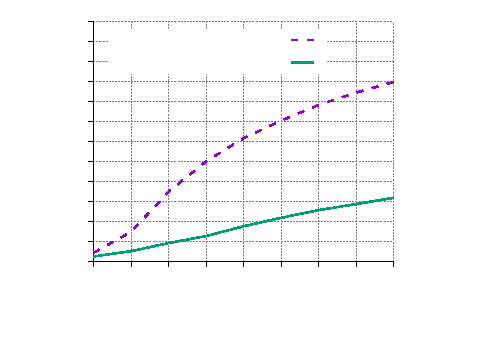
\includegraphics{figures/concat-graph-data.pdf}}%
    \gplfronttext
  \end{picture}%
\endgroup

    \end{subfigure}%
    \hspace{-20pt}
    \begin{subfigure}[t]{0.5\textwidth}
        \centering
        % GNUPLOT: LaTeX picture with Postscript
\begingroup
  \makeatletter
  \providecommand\color[2][]{%
    \GenericError{(gnuplot) \space\space\space\@spaces}{%
      Package color not loaded in conjunction with
      terminal option `colourtext'%
    }{See the gnuplot documentation for explanation.%
    }{Either use 'blacktext' in gnuplot or load the package
      color.sty in LaTeX.}%
    \renewcommand\color[2][]{}%
  }%
  \providecommand\includegraphics[2][]{%
    \GenericError{(gnuplot) \space\space\space\@spaces}{%
      Package graphicx or graphics not loaded%
    }{See the gnuplot documentation for explanation.%
    }{The gnuplot epslatex terminal needs graphicx.sty or graphics.sty.}%
    \renewcommand\includegraphics[2][]{}%
  }%
  \providecommand\rotatebox[2]{#2}%
  \@ifundefined{ifGPcolor}{%
    \newif\ifGPcolor
    \GPcolortrue
  }{}%
  \@ifundefined{ifGPblacktext}{%
    \newif\ifGPblacktext
    \GPblacktexttrue
  }{}%
  % define a \g@addto@macro without @ in the name:
  \let\gplgaddtomacro\g@addto@macro
  % define empty templates for all commands taking text:
  \gdef\gplbacktext{}%
  \gdef\gplfronttext{}%
  \makeatother
  \ifGPblacktext
    % no textcolor at all
    \def\colorrgb#1{}%
    \def\colorgray#1{}%
  \else
    % gray or color?
    \ifGPcolor
      \def\colorrgb#1{\color[rgb]{#1}}%
      \def\colorgray#1{\color[gray]{#1}}%
      \expandafter\def\csname LTw\endcsname{\color{white}}%
      \expandafter\def\csname LTb\endcsname{\color{black}}%
      \expandafter\def\csname LTa\endcsname{\color{black}}%
      \expandafter\def\csname LT0\endcsname{\color[rgb]{1,0,0}}%
      \expandafter\def\csname LT1\endcsname{\color[rgb]{0,1,0}}%
      \expandafter\def\csname LT2\endcsname{\color[rgb]{0,0,1}}%
      \expandafter\def\csname LT3\endcsname{\color[rgb]{1,0,1}}%
      \expandafter\def\csname LT4\endcsname{\color[rgb]{0,1,1}}%
      \expandafter\def\csname LT5\endcsname{\color[rgb]{1,1,0}}%
      \expandafter\def\csname LT6\endcsname{\color[rgb]{0,0,0}}%
      \expandafter\def\csname LT7\endcsname{\color[rgb]{1,0.3,0}}%
      \expandafter\def\csname LT8\endcsname{\color[rgb]{0.5,0.5,0.5}}%
    \else
      % gray
      \def\colorrgb#1{\color{black}}%
      \def\colorgray#1{\color[gray]{#1}}%
      \expandafter\def\csname LTw\endcsname{\color{white}}%
      \expandafter\def\csname LTb\endcsname{\color{black}}%
      \expandafter\def\csname LTa\endcsname{\color{black}}%
      \expandafter\def\csname LT0\endcsname{\color{black}}%
      \expandafter\def\csname LT1\endcsname{\color{black}}%
      \expandafter\def\csname LT2\endcsname{\color{black}}%
      \expandafter\def\csname LT3\endcsname{\color{black}}%
      \expandafter\def\csname LT4\endcsname{\color{black}}%
      \expandafter\def\csname LT5\endcsname{\color{black}}%
      \expandafter\def\csname LT6\endcsname{\color{black}}%
      \expandafter\def\csname LT7\endcsname{\color{black}}%
      \expandafter\def\csname LT8\endcsname{\color{black}}%
    \fi
  \fi
    \setlength{\unitlength}{0.0500bp}%
    \ifx\gptboxheight\undefined%
      \newlength{\gptboxheight}%
      \newlength{\gptboxwidth}%
      \newsavebox{\gptboxtext}%
    \fi%
    \setlength{\fboxrule}{0.5pt}%
    \setlength{\fboxsep}{1pt}%
\begin{picture}(4680.00,3276.00)%
    \gplgaddtomacro\gplbacktext{%
      \csname LTb\endcsname%%
      \put(721,751){\makebox(0,0)[r]{\strut{}$\sfrac{1}{16}$}}%
      \csname LTb\endcsname%%
      \put(721,943){\makebox(0,0)[r]{\strut{}$\sfrac{1}{8}$}}%
      \csname LTb\endcsname%%
      \put(721,1135){\makebox(0,0)[r]{\strut{}$\sfrac{1}{4}$}}%
      \csname LTb\endcsname%%
      \put(721,1327){\makebox(0,0)[r]{\strut{}$\sfrac{1}{2}$}}%
      \csname LTb\endcsname%%
      \put(721,1519){\makebox(0,0)[r]{\strut{}1}}%
      \csname LTb\endcsname%%
      \put(721,1711){\makebox(0,0)[r]{\strut{}2}}%
      \csname LTb\endcsname%%
      \put(721,1903){\makebox(0,0)[r]{\strut{}4}}%
      \csname LTb\endcsname%%
      \put(721,2095){\makebox(0,0)[r]{\strut{}8}}%
      \csname LTb\endcsname%%
      \put(721,2287){\makebox(0,0)[r]{\strut{}16}}%
      \csname LTb\endcsname%%
      \put(721,2479){\makebox(0,0)[r]{\strut{}32}}%
      \csname LTb\endcsname%%
      \put(721,2671){\makebox(0,0)[r]{\strut{}64}}%
      \csname LTb\endcsname%%
      \put(721,2863){\makebox(0,0)[r]{\strut{}128}}%
      \csname LTb\endcsname%%
      \put(721,3055){\makebox(0,0)[r]{\strut{}256}}%
      \csname LTb\endcsname%%
      \put(900,484){\makebox(0,0){\strut{}0}}%
      \csname LTb\endcsname%%
      \put(1260,484){\makebox(0,0){\strut{}}}%
      \csname LTb\endcsname%%
      \put(1620,484){\makebox(0,0){\strut{}100}}%
      \csname LTb\endcsname%%
      \put(1980,484){\makebox(0,0){\strut{}}}%
      \csname LTb\endcsname%%
      \put(2340,484){\makebox(0,0){\strut{}200}}%
      \csname LTb\endcsname%%
      \put(2699,484){\makebox(0,0){\strut{}}}%
      \csname LTb\endcsname%%
      \put(3059,484){\makebox(0,0){\strut{}300}}%
      \csname LTb\endcsname%%
      \put(3419,484){\makebox(0,0){\strut{}}}%
      \csname LTb\endcsname%%
      \put(3779,484){\makebox(0,0){\strut{}400}}%
    }%
    \gplgaddtomacro\gplfronttext{%
      \csname LTb\endcsname%%
      \put(391,1903){\rotatebox{-270}{\makebox(0,0){\strut{}}}}%
      \put(2339,154){\makebox(0,0){\strut{}Number of columns}}%
      \csname LTb\endcsname%%
      \put(3286,1118){\makebox(0,0)[r]{\strut{}implicit join}}%
      \csname LTb\endcsname%%
      \put(3286,898){\makebox(0,0)[r]{\strut{}dependent join}}%
    }%
    \gplbacktext
    \put(0,0){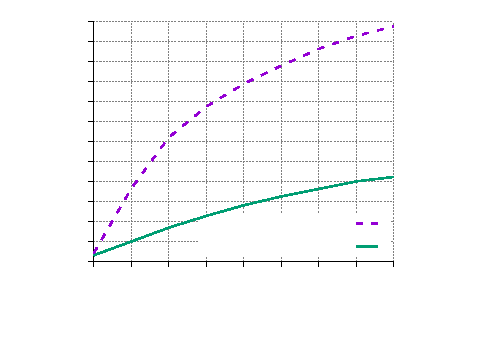
\includegraphics{figures/join-graph-data.pdf}}%
    \gplfronttext
  \end{picture}%
\endgroup

    \end{subfigure}
    \caption{#1}
    \label{fig:dependentVsImplicitBenchmarks}
  \end{figure}
}

\newcommand{\goodreducescalacodesection}{\lstinputlisting[style=scala, firstline=3, lastline=4, breaklines]{scala/src/main/scala/goodreduce.scala}}
\newcommand{\shapecodesection}{\lstinputlisting[style=scala, firstline=8, lastline=11, breaklines]{scala/src/main/scala/numpy.scala}}
\newcommand{\datatypecodesection}{\lstinputlisting[style=scala, firstline=19, lastline=19, breaklines]{scala/src/main/scala/numpy.scala}}
\newcommand{\ndarraycodesection}{\lstinputlisting[style=scala, firstline=23, lastline=23, breaklines]{scala/src/main/scala/numpy.scala}}
\newcommand{\randomnormalcodesection}{\lstinputlisting[style=scala, firstline=27, lastline=27, breaklines]{scala/src/main/scala/numpy.scala}}
\newcommand{\multiplycodesection}{\lstinputlisting[style=scala, firstline=31, lastline=31, breaklines]{scala/src/main/scala/numpy.scala}}
\newcommand{\numelementscodesection}{\lstinputlisting[style=scala, firstline=36, lastline=40, breaklines]{scala/src/main/scala/numpy.scala}}
\newcommand{\reshapecodesection}{\lstinputlisting[style=scala, firstline=44, lastline=45, breaklines]{scala/src/main/scala/numpy.scala}}
\newcommand{\reducecodesection}{\lstinputlisting[style=scala, firstline=50, lastline=66, breaklines]{scala/src/main/scala/numpy.scala}}
\newcommand{\npmeancodesection}{\lstinputlisting[style=scala, firstline=86, lastline=87, breaklines]{scala/src/main/scala/numpy.scala}}
\newcommand{\badreducescalacodesection}{\lstinputlisting[style=scala, firstline=2, lastline=4, breaklines]{scala/src/test/scala/badreduce.scala}}

\hfuzz=0.5pt

%%%%%%%%%%%%%%%%%%%%%%%%%%%%%%%%%%%%%%%%%%%%%%%%%%
%%%%%%%%%%%%%% TypeOf paper headers %%%%%%%%%%%%%%
%%%%%%%%%%%%%%%%%%%%%%%%%%%%%%%%%%%%%%%%%%%%%%%%%%

\newcommand{\oursystem}{$\lambda${\tiny $\mathop{\protect\vphantom{X}}^\text{nd}_{<:\{\}}$}\xspace}
\newcommand\FR{System~FR\xspace}
\newcommand\singleton[1]{\lbrace #1 \rbrace}
\usepackage{xfrac}
\usepackage{caption}
\usepackage{subcaption}
\usepackage{upgreek} % for \textmu


\begin{document}

\frontmatter
\begin{titlepage}
\begin{otherlanguage}{french}
\begin{center}
\sffamily
\null\vspace{2cm}
\huge Abstractions for Type-Level Programming\\[24pt]
\textcolor{gray}{\small THIS IS A TEMPORARY TITLE PAGE\\
It will be replaced for the final print by a version\\[-14pt]
provided by the registrar's office.}
\vfill
\normalsize THÈSE N. TBD (\the\year)\\[10pt]
PRÉSENTÉE LE {\MakeUppercase\today}\\
À LA FACULTÉ INFORMATIQUE ET COMMUNICATIONS\\
LABORATOIRE DE MÉTHODES DE PROGRAMMATION\\
PROGRAMME DOCTORAL EN INFORMATIQUE ET COMMUNICATIONS\\[10pt]
ÉCOLE POLYTECHNIQUE FÉDÉRALE DE LAUSANNE\\
pour l'obtention du grade de Docteur ès Sciences\\
par\\[20pt]
\Large Olivier Blanvillain\\[20pt]
\small acceptée sur proposition du jury:\\[4pt]
Prof Name Surname, président du jury\\
Prof Name Surname, directeur de thèse\\
Prof Name Surname, rapporteur\\
Prof Name Surname, rapporteur\\
Prof Name Surname, rapporteur\\[12pt]
Lausanne, EPFL, \the\year
\end{center}
\vspace{2cm}
\end{otherlanguage}
\end{titlepage}


\setcounter{page}{0}

\chapter{Acknowledgements}
\lipsum[1-2]
Here's an example how to cite.~\cite{atc13}

\bigskip
\noindent\textit{Lausanne, \today}
\hfill Olivier Blanvillain

\cleardoublepage
\chapter*{Abstract}
\markboth{Abstract}{Abstract}
\addcontentsline{toc}{chapter}{Abstract (English/Français)}
\lipsum[1-2] % max 3499 characters
\begin{otherlanguage}{french}
\cleardoublepage
\chapter*{Résumé}
\markboth{Résumé}{Résumé}
\lipsum[1-2]
\end{otherlanguage}

\tableofcontents

\cleardoublepage
\phantomsection
\addcontentsline{toc}{chapter}{List of Figures}
\listoffigures
\mainmatter

%%%%%%%%%%%%%%%%%%%%%%%%%%%%%%%%%%%%%%%%%%%%%%%%%%
%%%%%%%%%%%%%%%%  Thesis Content  %%%%%%%%%%%%%%%%
%%%%%%%%%%%%%%%%%%%%%%%%%%%%%%%%%%%%%%%%%%%%%%%%%%

\chapter{Introduction}
\lipsum[1]

\chapter{(Ab)Using Implicits}
\lipsum[1]

\chapter{A Dependently Typed Extension of Scala Based on Singleton Types}
\lipsum[1]

\chapter{Type-Level Programming With Match Types}
\lipsum[1]
\begin{lemma}[Permutation]
  \lbl{lem:permutation}
  ~\\[10pt]\indent
  If $\Γ$ and $\Δ$ are well-formed and $\Δ$ is a permutation of $\Γ$, then:
  \begin{enumerate}
    \item % 0
    If   $\Γ \⊢ \disj(\S, \T)$,
    then $\Δ \⊢ \disj(\S, \T)$.

    \item % 1
    If   $\Γ \⊢ \S \<: \T$,
    then $\Δ \⊢ \S \<: \T$.

    \item % 2
    If   $\Γ \⊢ \t \: \T$,
    then $\Δ \⊢ \t \: \T$.
  \end{enumerate}
\end{lemma}

\begin{proof}
  We prove 1. and 2. simultaneously by induction on two derivations of $\Γ \⊢ \disj(\V, \W)$ and $\Γ \⊢ \S \<: \T$.
  More precisely, the induction is done on the cumulative depth of both derivation tree.
  \begin{enumerate}
    \item % 0
    $\Γ \⊢ \disj(\V, \W)$
    \begin{itemize}
      \Case\DXi:
      \quad $\V \= \C_{1}$
      \quad $\W \= \C_{2}$
      \quad $\(\C_{1}, \C_{2}) \∈ \Ξ$

      Using \DXi with context $\Δ$ directly leads to the desired result.

      \Case\DPsi:
      \quad $\V \= \{ \new \C_{1} \}$
      \quad $\W \= \C_{2}$
      \quad $\(\C_{1}, \C_{2}) \∉ \Ψ$

      Using \DPsi with context $\Δ$ directly leads to the desired result.

      \Case\DSub:
      \quad $\Γ \⊢ \V \<: \U$
      \quad $\Γ \⊢ \disj(\U, \W)$

      By the IH we get $\Δ \⊢ \disj(\U, \W)$.
      Using the 2nd part of the lemma we obtain $\Δ \⊢ \V \<: \U$.
      The result follows from \DSub.

      \Case\DArrow:
      \quad $\V \= \V_{1} \→ \V_{2}$
      \quad $\W \= \C$

      Using \DArrow with context $\Δ$ directly leads to the desired result.

      \Case\DAll:
      \quad $\V \= \∀ \X \<: \V_{1}.~ \V_{2}$
      \quad $\W \= \C$

      Using \DAll with context $\Δ$ directly leads to the desired result.
    \end{itemize}

    \item % 1
    $\Γ \⊢ \S \<: \T$.
    \begin{itemize}
      \Case\SRefl:
      \quad $\T \= \S$

      Using \SRefl with context $\Δ$ directly leads to the desired result.

      \Case\STrans:
      \quad $\Γ \⊢ \S \<: \U$
      \quad $\Γ \⊢ \U \<: \T$

      The result follows directly from the IH and \STrans.

      \Case\STop:
      \quad $\T \= \Top$

      Using \STop with context $\Δ$ directly leads to the desired result.

      \Case\SSin:
      \quad $\S \= \{ \new \C \}$
      \quad $\T \= \C$

      Using \SSin with context $\Δ$ directly leads to the desired result.

      \Case\STvar:
      \quad $\S \= \X$
      \quad $\X \<: \T \∈ \Γ$
      Since $\Δ$ is a permutation of $\Γ$, $\X \<: \T \∈ \Δ$, and the result follows from \STvar.

      \Case\SArrow:
      \quad $\S \= \S_{1} \→ \S_{2}$
      \quad $\T \= \T_{1} \→ \T_{2}$
      \\\phantom{\textit{Case}~\SArrow:}
      \quad $\Γ \⊢ \T_{1} \<: \S_{1}$
      \quad $\Γ \⊢ \S_{2} \<: \T_{2}$

      The result follows directly from the IH and \SArrow.

      \Case\SAll:
      \quad $\S \= \∀ \X \<: \U_{1}.~ \S_{2}$
      \quad $\T \= \∀ \X \<: \U_{1}.~ \T_{2}$
      \quad $\Γ, \X \<: \U_{1} \⊢ \S_{2} \<: \T_{2}$

      If $\Δ$ is a permutation of $\Γ$, then $\Δ, \X \<: \U_{1}$ is a permutation of $\Γ, \X \<: \U_{1}$.
      Therefore, we can use the IH to get $\Δ, \X \<: \U_{1} \⊢ \S_{2} \<: \T_{2}$.
      The result follows from \SAll.

      \Case\SPsi:
      \quad $\S \= \C_{1}$
      \quad $\T \= \C_{2}$
      \quad $\(\C_{1}, \C_{2}) \∈ \Ψ$

      Using \SPsi with context $\Δ$ directly leads to the desired result.

      \Case\SMatch1/2:
      \quad $\T_{1} \= \T_n$
      \quad $\T_{2} \= \T_s \match \{ \S_i \⇒ \T_i \} \otherwise \T_d$
      \\\phantom{\textit{Case}~\SMatch1/2:}
      \quad $\Γ \⊢ \T_s \<: \S_n$
      \quad $\∀ \m<n.~ \Γ \⊢ \disj(\T_s, \S_m)$

      By the 1st part of the lemma we get $\∀ \m<n.~ \Δ \⊢ \disj(\T_s, \S_m)$.
      From the IH we obtain $\Δ \⊢ \T_s \<: \S_n$.
      The result follows from \SMatch1/2.

      \Case\SMatch3/4:
      \quad $\S \= \T_d$
      \quad $\T \= \T_s \match \{ \S_i \⇒ \T_i \} \otherwise \T_d$
      \quad $\∀ \n.~ \Γ \⊢ \disj(\T_s, \S_n)$

      The result follows from the 1st part of the lemma and \SMatch3/4.

      \Case\SMatch5:
      \quad $\S \= \S_s \match \{ \U_i \⇒ \S_i \} \otherwise \S_d$
      \quad $\T \= \T_s \match \{ \U_i \⇒ \T_i \} \otherwise \T_d$
      \\\phantom{\textit{Case}~\SMatch5:}
      \quad $\Γ \⊢ \S_s \<: \T_s$
      \quad $\∀ \n.~ \Γ \⊢ \S_n \<: \T_n$
      \quad $\Γ \⊢ \S_d \<: \T_d$

      The result follows directly from the IH and \SMatch5.
    \end{itemize}

    \item % 2
    By induction on a derivation of $\Γ \⊢ \t \: \T$
    \begin{itemize}
      \Case\TVar:
      \quad $\t \= \x$
      \quad $\x \: \T \∈ \Γ$

      Since $\Δ$ is a permutation of $\Γ$, $\x \: \T \∈ \Δ$, and the result follows from \TVar.

      \Case\TAbs:
      \quad $\t \= \λ \x \: \T_{1} \t_{2}$
      \quad $\T \= \T_{1} \→ \T_{2}$
      \quad $\Γ, \x \: \T_{1} \⊢ \t_{2} \: \T_{2}$

      If $\Δ$ is a permutation of $\Γ$, then $\Δ, \x \: \T_{1}$ is a permutation of $\Γ, \x \: \T_{1}$.
      Therefore, we can use the IH to get $\Δ, \x \: \T_{1} \⊢ \t_{2} \: \T_{2}$.
      The result follows from \TAbs.

      \Case\TApp:
      \quad $\t \= \t_{1} \t_{2}$
      \quad $\T \= \T_{12}$
      \quad $\Γ \⊢ \t_{1} \: \T_{11} \→ \T_{12}$
      \quad $\Γ \⊢ \t_{2} \: \T_{11}$

      The result follows directly from the IH and \TApp.

      \Case\TTAbs:
      \quad $\t \= \λ \X \<: \U_{1}.~ \t_{2}$
      \quad $\T \= \∀ \X \<: \U_{1}.~ \T_{2}$
      \quad $\Γ, \X \<: \U_{1} \⊢ \t_{2} \: \T_{2}$

      If $\Δ$ is a permutation of $\Γ$, then $\Δ, \X \<: \U_{1}$ is a permutation of $\Γ, \X \<: \U_{1}$.
      Therefore, we can use the IH to get $\Δ, \X \<: \U_{1} \⊢ \t_{2} \: \T_{2}$.
      The result follows from \TTAbs.

      \Case\TTApp:
      \quad $\t \= \t_{1} \T_{2}$
      \quad $\T \= \[\X \↦ \T_{2}] \T_{12}$
      \\\phantom{\textit{Case}~\TTApp:}
      \quad $\Γ \⊢ \t_{1} \: \(\∀ \X \<: \U_{1}.~ \T_{12})$
      \quad $\Γ \⊢ \T_{2} \<: \U_{1}$

      By the IH we get $\Δ \⊢ \t_{1} \: \(\∀ \X \<: \U_{1}.~ \T_{12})$.
      Using the 2nd part of the lemma we obtain $\Δ \⊢ \T_{2} \<: \U_{1}$.
      The result follows from \TTApp.

      \Case\TSub:
      \quad $\Γ \⊢ \t \: \S$
      \quad $\Γ \⊢ \S \<: \T$

      By the IH we get $\Δ \⊢ \t \: \S$.
      Using the 2nd part of the lemma we obtain $\Δ \⊢ \S \<: \T$.
      The result follows from \TSub.

      \Case\TClass:
      \quad $\t \= \new \C$
      \quad $\T \= \{ \new \C \}$

      Using \TClass with context $\Δ$ directly leads to the desired result.

      \Case\TMatch:
      \quad $\t \= \t_s \match \{ \x_i \: \C_i \⇒ \t_i \} \otherwise \t_d$
      \quad $\T \= \T_s \match \{ \C_i \⇒ \T_i \} \otherwise \T_d$
      \\\phantom{\textit{Case}~\TMatch:}
      \quad $\Γ \⊢ \t_s \: \T_s$
      \quad $\Γ, \x_i \: \C_i \⊢ \t_i \: \T_i$
      \quad $\Γ \⊢ \t_d \: \T_d$

      If $\Δ$ is a permutation of $\Γ$, then $\Δ, \x_i \: \C_i$ is a permutation of $\Γ, \x_i \: \C_i$. Therefore the result follows directly from the IH and \TMatch.
    \end{itemize}
  \end{enumerate}
\end{proof}

\begin{lemma}[Weakening]
  \lbl{lem:weakening}~
  \begin{enumerate}
    \item % 0
    If $\Γ \⊢ \disj(\S, \T)$ and $\Γ, \X \<: \U$ is well formed,
    then $\Γ, \X \<: \U \⊢ \disj(\S, \T)$.

    \item % 1
    If $\Γ \⊢ \S \<: \T$ and $\Γ, \X \<: \U$ is well formed,
    then $\Γ, \X \<: \U \⊢ \S \<: \T$.

    \item % 2
    If $\Γ \⊢ \S \<: \T$ and $\Γ, \x \: \U$ is well formed,
    then $\Γ, \x \: \U \⊢ \S \<: \T$.

    \item % 3
    If $\Γ \⊢ \t \: \T$ and $\Γ, \x \: \U$ is well formed,
    then $\Γ, \x \: \U \⊢ \t \: \T$.

    \item % 4
    If $\Γ \⊢ \t \: \T$ and $\Γ, \X \<: \U$ is well formed,
    then $\Γ, \X \<: \U \⊢ \t \: \T$.
  \end{enumerate}
\end{lemma}

\begin{proof}
  We prove 1. and 2. simultaneously by induction on two derivations of $\Γ \⊢ \disj(\V, \W)$ and $\Γ \⊢ \S \<: \T$.
  More precisely, the induction is done on the cumulative depth of both derivation tree.
  \begin{enumerate}
    \item % 0
    $\Γ \⊢ \disj(\V, \W)$
    \begin{itemize}
      \Case\DXi:
      \quad $\V \= \C_{1}$
      \quad $\W \= \C_{2}$
      \quad $\(\C_{1}, \C_{2}) \∈ \Ξ$

      Using \DXi with context $\Γ, \X \<: \U$ directly leads to the desired result.

      \Case\DPsi:
      \quad $\V \= \{ \new \C_{1} \}$
      \quad $\W \= \C_{2}$
      \quad $\(\C_{1}, \C_{2}) \∉ \Ψ$

      Using \DPsi with context $\Γ, \X \<: \U$ directly leads to the desired result.

      \Case\DSub:
      \quad $\Γ \⊢ \V \<: \U$
      \quad $\Γ \⊢ \disj(\U, \W)$

      By the IH we get $\Γ \⊢ \disj(\U, \W)$.
      Using the 2nd part of the lemma we obtain $\Γ, \X \<: \U \⊢ \V \<: \U$.
      The result follows from \DSub.

      \Case\DArrow:
      \quad $\V \= \V_{1} \→ \V_{2}$
      \quad $\W \= \C$

      Using \DArrow with context $\Γ, \X \<: \U$ directly leads to the desired result.

      \Case\DAll:
      \quad $\V \= \∀ \X \<: \V_{1}.~ \V_{2}$
      \quad $\W \= \C$

      Using \DAll with context $\Γ, \X \<: \U$ directly leads to the desired result.
    \end{itemize}

    \item % 1
    $\Γ \⊢ \S \<: \T$.
    \begin{itemize}
      \Case\SRefl:
      \quad $\T \= \S$

      Using \SRefl with context $\Γ, \X \<: \U$ directly leads to the desired result.

      \Case\STrans:
      \quad $\Γ \⊢ \S \<: \U$
      \quad $\Γ \⊢ \U \<: \T$

      The result follows from the IH and \STrans.

      \Case\STop:
      \quad $\T \= \Top$

      Using \STop with context $\Γ, \X \<: \U$ directly leads to the desired result.

      \Case\SSin:
      \quad $\S \= \{ \new \C \}$
      \quad $\T \= \C$

      Using \SSin with context $\Γ, \X \<: \U$ directly leads to the desired result.

      \Case\STvar:
      \quad $\S \= \Y$
      \quad $\Y \<: \T \∈ \Γ$

      If $\Y \<: \T \∈ \Γ$, then $\Y \<: \T \∈ \Γ, \X \<: \U$ and the result follows from \STvar.

      \Case\SArrow:
      \quad $\S \= \S_{1} \→ \S_{2}$
      \quad $\T \= \T_{1} \→ \T_{2}$
      \\\phantom{\textit{Case}~\SArrow:}
      \quad $\Γ \⊢ \T_{1} \<: \S_{1}$
      \quad $\Γ \⊢ \S_{2} \<: \T_{2}$

      The result follows from the IH and \SArrow.

      \Case\SAll:
      \quad $\S \= \∀ \Y \<: \U_{1}.~ \S_{2}$
      \quad $\T \= \∀ \Y \<: \U_{1}.~ \T_{2}$
      \quad $\Γ, \Y \<: \U_{1} \⊢ \S_{2} \<: \T_{2}$

      Using the IH with context $\Γ_{IH} \= \Γ, \Y \<: \U_{1}$, we get $\Γ, \Y \<: \U_{1}, \X \<: \U \⊢ \S_{2} \<: \T_{2}$.
      From \Cref{lem:permutation}, $\Γ, \X \<: \U, \Y \<: \U_{1} \⊢ \S_{2} \<: \T_{2}$
      The result follows from \SAll.

      \Case\SPsi:
      \quad $\S \= \C_{1}$
      \quad $\T \= \C_{2}$
      \quad $\(\C_{1}, \C_{2}) \∈ \Ψ$

      Using \SPsi with context $\Γ, \X \<: \U$ directly leads to the desired result.

      \Case\SMatch1/2:
      \quad $\T_{1} \= \T_n$
      \quad $\T_{2} \= \T_s \match \{ \S_i \⇒ \T_i \} \otherwise \T_d$
      \\\phantom{\textit{Case}~\SMatch1/2:}
      \quad $\Γ \⊢ \T_s \<: \S_n$
      \quad $\∀ \m<n.~ \Γ \⊢ \disj(\T_s, \S_m)$

      From the IH we get $\Γ, \X \<: \U \⊢ \T_s \<: \S_n$.
      Using the 1st part of the lemma we obtain $\∀ \m< \n.~\ \Γ, \X \<: \U \⊢ \disj(\T_s, \S_m)$.
      The result follows from \SMatch1/2.

      \Case\SMatch3/4:
      \quad $\T_{1} \= \T_d$
      \quad $\T_{2} \= \T_s \match \{ \S_i \⇒ \T_i \} \otherwise \T_d$
      \quad $\∀ \n.~ \Γ \⊢ \disj(\T_s, \S_n)$

      Using the 1st part of the lemma we get $\∀ \n.~\ \Γ, \X \<: \U \⊢ \disj(\T_s, \S_n)$.
      The result follows from \SMatch3/4.

      \Case\SMatch5:
      \quad $\S \= \S_s \match \{ \S_i \⇒ \T_i \} \otherwise \T_d$
      \quad $\T \= \T_s \match \{ \S_i \⇒ \U_i \} \otherwise \U_d$
      \\\phantom{\textit{Case}~\SMatch5:}
      \quad $\Γ \⊢ \S_s \<: \T_s$
      \quad $\∀ \n.~ \Γ \⊢ \T_n \<: \U_n$
      \quad $\Γ \⊢ \T_d \<: \U_d$

      We use the IH on each premise and the result follows directly from \SMatch5.
    \end{itemize}

    \item % 2
    By inspection of the subtyping rules, it is clear that typing assumbtions play no role in subtyping derivations.

    \item % 3
    By induction on a derivation of $\Γ \⊢ \t \: \T$.
    \begin{itemize}
      \Case\TVar:
      \quad $\t \= \y$
      \quad $\y \: \T \∈ \Γ$

      If $\y \: \T \∈ \Γ$ then $\y \: \T \∈ \Γ, \x \: \U$ and the result follows from \TVar.

      \Case\TAbs:
      \quad $\t \= \λ \y \: \T_{1} \t_{2}$
      \quad $\T \= \T_{1} \→ \T_{2}$
      \quad $\Γ, \y \: \T_{1} \⊢ \t_{2} \: \T_{2}$

      Using the IH with $\Γ_{IH} \= \Γ, \y \: \T_{1}$ we get $\Γ, \y \: \T_{1}, \x \: \U \⊢ \t_{2} \: \T_{2}$.
      From \Cref{lem:permutation}, $\Γ, \x \: \U, \y \: \T_{1} \⊢ \t_{2} \: \T_{2}$.
      The result follows from \TAbs.

      \Case\TApp:
      \quad $\t \= \t_{1} \t_{2}$
      \quad $\T \= \T_{12}$
      \quad $\Γ \⊢ \t_{1} \: \T_{11} \→ \T_{12}$
      \quad $\Γ \⊢ \t_{2} \: \T_{12}$

      We use the IH on each premise and the result follows from \TApp.

      \Case\TTAbs:
      \quad $\t \= \λ \X \<: \T_{1}.~ \t_{2}$
      \quad $\T \= \∀ \X \<: \T_{1}.~ \T_{2}$
      \quad $\Γ, \X \<: \T_{1} \⊢ \t_{2} \: \T_{2}$

      Using the IH with $\Γ_{IH} \= \Γ, \X \<: \T_{1}$ we get $\Γ, \X \<: \T_{1}, \x \: \U \⊢ \t_{2} \: \T_{2}$.
      From \Cref{lem:permutation}, $\Γ, \x \: \U, \X \<: \T_{1} \⊢ \t_{2} \: \T_{2}$
      The result follows from \TTAbs.

      \Case\TTApp:
      \quad $\t \= \t_{1} \T_{2}$
      \quad $\T \= \[\X \↦ \T_{2}] \T_{12}$
      \\\phantom{\textit{Case}~\TTApp:}
      \quad $\Γ \⊢ \t_{1} \: \(\∀ \X \<: \T_{11}.~ \T_{12})$
      \quad $\Γ \⊢ \T_{2} \<: \T_{11}$

      Using the IH on the left premise we get $\Γ, \x \: \U \⊢ \t_{1} \: \(\∀ \X \<: \T_{11}.~ \T_{12})$.
      Using the 3rd part of the lemma on the right premise we obtain $\Γ, \x \: \U \⊢ \T_{2} \<: \T_{11}$.
      The result follows from \TTApp.

      \Case\TSub:
      \quad $\Γ \⊢ \t \: \S$
      \quad $\Γ \⊢ \S \<: \T$

      Using the IH on the left premise we get $\Γ, \x \: \U \⊢ \t \: \S$.
      Using the 3rd part of the lemma on the right premise we obtain $\Γ, \x \: \U \⊢ \S \<: \T$.
      The result follows from \TSub.

      \Case\TClass:
      \quad $\t \= \new \C$
      \quad $\T \= \{ \new \C \}$

      Using \TClass with context $\Γ, \x \: \U$ directly leads to the desired result.

      \Case\TMatch:
      \quad $\t \= \t_s \match \{ \x_i \: \C_i \⇒ \t_i \} \otherwise \t_d$
      \quad $\T \= \T_s \match \{ \C_i \⇒ \T_i \} \otherwise \T_d$
      \\\phantom{\textit{Case}~\TMatch:}
      \quad $\Γ \⊢ \t_s \: \T_s$
      \quad $\Γ, \x_i \: \C_i \⊢ \t_i \: \T_i$
      \quad $\Γ \⊢ \t_d \: \T_d$

      We use the IH on each premise and the result follows directly from \Cref{lem:permutation} and \TMatch.
    \end{itemize}

    \item % 4
    By induction on a derivation of $\Γ \⊢ \t \: \T$.
    \begin{itemize}
      \Case\TVar:
      \quad $\t \= \x$
      \quad $\x \: \T \∈ \Γ$

      If $\y \: \T \∈ \Γ$ then $\y \: \T \∈ \Γ, \X \<: \U$ and the result follows from \TVar.

      \Case\TAbs:
      \quad $\t \= \λ \x \: \T_{1} \t_{2}$
      \quad $\T \= \T_{1} \→ \T_{2}$
      \quad $\Γ, \x \: \T_{1} \⊢ \t_{2} \: \T_{2}$

      Using the IH with $\Γ_{IH} \= \Γ, \x \: \T_{1}$ we get $\Γ, \x \: \T_{1}, \X \<: \U \⊢ \t_{2} \: \T_{2}$.
      From \Cref{lem:permutation}, $\Γ, \X \<: \U, \x \: \T_{1} \⊢ \t_{2} \: \T_{2}$.
      The result follows from \TAbs.

      \Case\TApp:
      \quad $\t \= \t_{1} \t_{2}$
      \quad $\T \= \T_{12}$
      \quad $\Γ \⊢ \t_{1} \: \T_{11} \→ \T_{12}$
      \quad $\Γ \⊢ \t_{2} \: \T_{12}$

      We use the IH on each premise and the result follows from \TApp.

      \Case\TTAbs:
      \quad $\t \= \λ \Y \<: \T_{1}.~ \t_{2}$
      \quad $\T \= \∀ \Y \<: \T_{1}.~ \T_{2}$
      \quad $\Γ, \Y \<: \T_{1} \⊢ \t_{2} \: \T_{2}$

      Using the IH with $\Γ_{IH} \= \Γ, \Y \<: \T_{1}$ we get $\Γ, \Y \<: \T_{1}, \X \<: \U \⊢ \t_{2} \: \T_{2}$.
      From \Cref{lem:permutation}, $\Γ, \X \<: \U, \Y \<: \T_{1}, \⊢ \t_{2} \: \T_{2}$.
      The result follows from \TTAbs.

      \Case\TTApp:
      \quad $\t \= \t_{1} \T_{2}$
      \quad $\T \= \[\Y \↦ \T_{2}] \T_{12}$
      \\\phantom{\textit{Case}~\TTApp:}
      \quad $\Γ \⊢ \t_{1} \: \(\∀ \Y \<: \T_{11}.~ \T_{12})$
      \quad $\Γ \⊢ \T_{2} \<: \T_{11}$

      Using the IH on the left premise we get $\Γ, \X \<: \U \⊢ \t_{1} \: \(\∀ \X \<: \T_{11}.~ \T_{12})$.
      Using the 2nd part of the lemma on the right premise we obtain $\Γ, \X \<: \U \⊢ \T_{2} \<: \T_{11}$.
      The result follows from \TTApp.

      \Case\TSub:
      \quad $\Γ \⊢ \t \: \S$
      \quad $\Γ \⊢ \S \<: \T$

      Using the IH on the left premise we get $\Γ, \S \<: \U \⊢ \t \: \S$.
      Using the 2nd part of the lemma on the right premise we obtain $\Γ, \X \<: \U \⊢ \S \<: \T$.
      The result follows from \TSub.

      \Case\TClass:
      \quad $\t \= \new \C$
      \quad $\T \= \{ \new \C \}$

      Using \TClass with context $\Γ, \X \<: \U$ directly leads to the desired result.

      \Case\TMatch:
      \quad $\t \= \t_s \match \{ \x_i \: \C_i \⇒ \t_i \} \otherwise \t_d$
      \quad $\T \= \T_s \match \{ \C_i \⇒ \T_i \} \otherwise \T_d$
      \\\phantom{\textit{Case}~\TMatch:}
      \quad $\Γ \⊢ \t_s \: \T_s$
      \quad $\Γ, \x_i \: \C_i \⊢ \t_i \: \T_i$
      \quad $\Γ \⊢ \t_d \: \T_d$

      We use the IH on each premise and the result follows directly from \Cref{lem:permutation} and \TMatch.
    \end{itemize}
  \end{enumerate}
\end{proof}

\begin{lemma}[Strengthening]
  \lbl{lem:strengthening}~

  If $\Γ, \x \: \T, \Δ \⊢ \S \<: \T$,
  then $\Γ, \Δ \⊢ \S \<: \T$.
\end{lemma}

\begin{proof}
  By inspection of the subtyping rules, it is clear that typing assumbtions play no role in subtyping derivations.

\end{proof}

\begin{lemma}[Substitution]
  \lbl{lem:substitution}~
  \begin{enumerate}
    \item % 0
    If $\Γ, \X \<: \Q, \Δ \⊢ \disj(\S, \T)$ and $\Γ \⊢ \P \<: \Q$,
    then $\Γ, \[\X \↦ \P] \Δ \⊢ \disj(\[\X \↦ \P] \S, \[\X \↦ \P] \T)$.

    \item % 1
    If $\Γ, \X \<: \Q, \Δ \⊢ \S \<: \T$ and $\Γ \⊢ \P \<: \Q$,
    then $\Γ, \[\X \↦ \P] \Δ \⊢ \[\X \↦ \P] \S \<: \[\X \↦ \P] \T$.

    \item % 2
    If $\Γ, \X \<: \Q, \Δ \⊢ \t \: \T$ and $\Γ \⊢ \P \<: \Q$,
    then $\Γ, \[\X \↦ \P] \Δ \⊢ \[\X \↦ \P] \t \: \[\X \↦ \P] \T$.

    \item % 3
    If $\Γ, \x \: \Q, \Δ \⊢ \t \: \T$ and $\Γ \⊢ \q \: \Q$,
    then $\Γ, \Δ \⊢ \[\x \↦ \q] \t \: \T$.
  \end{enumerate}
\end{lemma}

\begin{proof}
  We prove 1. and 2. simultaneously by induction on two derivations of $\Γ, \X \<: \Q, \Δ \⊢ \disj(\V, \W)$ and $\Γ, \X \<: \Q, \Δ \⊢ \S \<: \T$.
  More precisely, the induction is done on the cumulative depth of both derivation tree.
  \begin{enumerate}
    \item % 0
    $\Γ, \X \<: \Q, \Δ \⊢ \disj(\V, \W)$
    \begin{itemize}
      \Case\DXi:
      \quad $\V \= \C_{1}$
      \quad $\W \= \C_{2}$
      \quad $\(\C_{1}, \C_{2}) \∈ \Ξ$

      Since $\[\X \↦ \P] \C_{1} \= \C_{1}$ and $\[\X \↦ \P] \C_{2} \= \C_{2}$, we can use \DXi with context $\Γ, \[\X \↦ \P] \Δ$ to obtain the desired result.

      \Case\DPsi:
      \quad $\V \= \{ \new \C_{1} \}$
      \quad $\W \= \C_{2}$
      \quad $\(\C_{1}, \C_{2}) \∉ \Ψ$

      Since $\[\X \↦ \P] \{ \new \C_{1} \} \= \{ \new \C_{1} \}$ and $\[\X \↦ \P] \C_{2} \= \C_{2}$, we can use \DPsi with context $\Γ, \[\X \↦ \P] \Δ$ to obtain the desired result.

      \Case\DSub:
      \quad $\Γ, \X \<: \Q, \Δ \⊢ \V \<: \U$
      \quad $\Γ, \X \<: \Q, \Δ \⊢ \disj(\U, \W)$

      By the IH we get $\Γ, \[\X \↦ \P] \Δ \⊢ \disj(\[\X \↦ \P] \U, \[\X \↦ \P] \W)$.
      Using the 2nd part of the lemma we obtain $\Γ, \[\X \↦ \P] \Δ \⊢ \[\X \↦ \P] \V \<: \[\X \↦ \P] \U$.
      The result follows from \DSub.

      \Case\DArrow:
      \quad $\V \= \V_{1} \→ \V_{2}$
      \quad $\W \= \C$

      Since $\[\X \↦ \P] \(\V_{1} \→ \V_{2}) \= \[\X \↦ \P] \V_{1} \→ \[\X \↦ \P] \V_{2}$ and $\[\X \↦ \P] \C \= \C$,
      we can use \DArrow with context $\Γ, \[\X \↦ \P] \Δ$ to obtain the desired result.

      \Case\DAll:
      \quad $\V \= \∀ \Y \<: \V_{1}.~ \V_{2}$
      \quad $\W \= \C$

      Since $\[\X \↦ \P] \(\∀ \Y \<: \V_{1}.~ \V_{2}) \= \∀ \Y \<: \[\X \↦ \P] \V_{1}.~ \[\X \↦ \P] \V_{2}$ and $\[\X \↦ \P] \C \= \C$,
      we can use \DAll with context $\Γ, \[\X \↦ \P] \Δ$ to obtain the desired result.
    \end{itemize}

    \item % 1
    $\Γ, \X \<: \Q, \Δ \⊢ \S \<: \T$.
    \begin{itemize}
      \Case\SRefl:
      \quad $\T \= \S$

      The result follows directly from \SRefl.

      \Case\STrans:
      \quad $\Γ, \X \<: \Q, \Δ \⊢ \S \<: \U$
      \quad $\Γ, \X \<: \Q, \Δ \⊢ \U \<: \T$

      The result follows directly from the IH and \STrans.

      \Case\STop:
      \quad $\T \= \Top$

      $\[\X \↦ \P] \Top \= \Top$ and the result follows from \STop.

      \Case\SSin:
      \quad $\S \= \{ \new \C \}$
      \quad $\T \= \C$

      $\[\X \↦ \P] \{ \new \C \} \= \{ \new \C \}$,
      $\[\X \↦ \P] \C \= \C$,
      and the result follows from \SSin.

      \Case\STvar:
      \quad $\S \= \Y$
      \quad $\Y \<: \T \∈ \(\Γ, \X \<: \Q, \Δ)$

      By context well-formedness, $\Y \<: \T \∈ \(\Γ, \X \<: \Q, \Δ)$ can be decomposed into 3 subcases:
      \begin{itemize}
        \Subcase $\Y \<: \T \∈ \Γ$:

        By context well-formedness $\X$ does not appear in $\Γ$ consequently is also absent from $\Y$ and $\T$.
        Hence $\Y \= \[\X \↦ \P] \Y$, $\T \= \[\X \↦ \P] \T$ and $\[\X \↦ \P] \Y \<: \[\X \↦ \P] \T \∈ \(\Γ, \[\X \↦ \P] \Δ)$.
        The result follows from \STvar.

        \Subcase $\Y \<: \T \∈ \Δ$:

        We have $\[\X \↦ \P] \Y \<: \[\X \↦ \P] \T \∈ \[\X \↦ \P] \Δ$ and $\[\X \↦ \P] \Y \<: \[\X \↦ \P] \T \∈ \(\Γ, \[\X \↦ \P] \Δ)$, and the result follows from \STvar.

        \Subcase $\Y \<: \T \= \X \<: \Q$ (\emph{i.e.} $\Y \= \X$ and $\T \= \Q$):

        By context well-formedness, $\X$ doesn't appear in $\Q$, and $\[\X \↦ \P] \T \= \[\X \↦ \P] \Q \= \Q$.
        Also $\[\X \↦ \P] \S \= \[\X \↦ \P] \X \= \P$ and $\[\X \↦ \P] \T \= \Q$.
        As a result, $\Γ \⊢ \P \<: \Q$ implies $\Γ \⊢ \[\X \↦ \P] \S \<: \[\X \↦ \P] \T$.
        Using \Cref{lem:weakening} we get $\Γ, \[\X \↦ \P] \Δ \⊢ \[\X \↦ \P] \S \<: \[\X \↦ \P] \T$, as required.

      \end{itemize}

      \Case\SArrow:
      \quad $\S \= \S_{1} \→ \S_{2}$
      \quad $\T \= \T_{1} \→ \T_{2}$
      \\\phantom{\textit{Case}~\SArrow:}
      \quad $\Γ, \X \<: \Q, \Δ \⊢ \T_{1} \<: \S_{1}$
      \quad $\Γ, \X \<: \Q, \Δ \⊢ \S_{2} \<: \T_{2}$

      $\[\X \↦ \P] \(\S_{1} \→ \S_{2}) \= \[\X \↦ \P] \S_{1} \→ \[\X \↦ \P] \S_{2}$,
      $\[\X \↦ \P] \(\T_{1} \→ \T_{2}) \= \[\X \↦ \P] \T_{1} \→ \[\X \↦ \P] \T_{2}$.
      The result follows from the IH and \SArrow.

      \Case\SAll:
      \quad $\S \= \∀ \Y \<: \U_{1}.~ \S_{2}$
      \quad $\T \= \∀ \Y \<: \U_{1}.~ \T_{2}$
      \quad $\Γ, \X \<: \Q, \Δ, \Y \<: \U_{1} \⊢ \S_{2} \<: \T_{2}$

      We instantiate the IH with $\Δ_{IH} \= \(\Δ, \Y \<: \U_{1})$ to obtain
      $\Γ, \[\X \↦ \P] \Δ, \Y \<: \[\X \↦ \P] \U_{1} \⊢ \[\X \↦ \P] \S_{2} \<: \[\X \↦ \P] \T_{2}$.
      Using \SAll, we get
      $\Γ, \[\X \↦ \P] \Δ \⊢ \(\∀ \Y \<: \[\X \↦ \P] \U_{1}.~ \[\X \↦ \P] \S_{2}) \<: \(\∀ \Y \<: \[\X \↦ \P] \U_{1}.~ \[\X \↦ \P] \T_{2})$, that is,
      $\Γ, \[\X \↦ \P] \Δ \⊢ \[\X \↦ \P] \(\∀ \Y \<: \U_{1}.~ \S_{2}) \<: \[\X \↦ \P] \(\∀ \Y \<: \U_{1}.~ \T_{2})$, as required.

      \Case\SPsi:
      \quad $\S \= \C_{1}$
      \quad $\T \= \C_{2}$
      \quad $\(\C_{1}, \C_{2}) \∈ \Ψ$

      $\[\X \↦ \P] \C_{1} \= \C_{1}$ and $\[\X \↦ \P] \C_{2} \= \C_{2}$. The result follows from \SPsi.

      \Case\SMatch1/2:
      \quad $\T_{1} \= \T_n$
      \quad $\T_{2} \= \T_s \match \{ \S_i \⇒ \T_i \} \otherwise \T_d$
      \\\phantom{\textit{Case}~\SMatch1/2:}
      \quad $\Γ, \X \<: \Q, \Δ \⊢ \T_s \<: \S_n$
      \quad $\∀ \m<n.~ \Γ, \X \<: \Q, \Δ \⊢ \disj(\T_s, \S_m)$

      Using the 1st part of the lemma we get $\∀ \m< \n.~ \Γ, \[\X \↦ \P] \Δ \⊢ \disj(\[\X \↦ \P] \T_s, \[\X \↦ \P] \S_m)$.
      By the IH we get $\Γ, \[\X \↦ \P] \Δ \⊢ \[\X \↦ \P] \T_s \<: \S_n$.
      $\[\X \↦ \P] \T \= \[\X \↦ \P] \T_s \match \{$ $\[\X \↦ \P] \S_i \⇒ \[\X \↦ \P] \T_i \} \otherwise \[\X \↦ \P] \T_d$,
      and the result follows from \SMatch1/2.

      \Case\SMatch3/4:
      \quad $\S \= \T_d$
      \quad $\T \= \T_s \match \{ \S_i \⇒ \T_i \} \otherwise \T_d$
      \\\phantom{\textit{Case}~\SMatch1/2:}
      \quad $\∀ \n.~ \Γ, \X \<: \Q, \Δ \⊢ \disj(\T_s, \S_n)$

      By the 1st part of the lemma we get $\∀ \n.~ \Γ, \[\X \↦ \P] \Δ \⊢ \disj(\[\X \↦ \P] \T_s, \[\X \↦ \P] \S_n)$ and the result follows from \SMatch3/4.

      \Case\SMatch5:
      \quad $\S \= \S_s \match \{ \U_i \⇒ \S_i \} \otherwise \S_d$
      \quad $\T \= \T_s \match \{ \U_i \⇒ \T_i \} \otherwise \T_d$
      \\\phantom{\textit{Case}~\SMatch5:}
      \quad $\Γ, \X \<: \Q, \Δ \⊢ \S_s \<: \T_s$
      \quad $\∀ \n.~ \Γ, \X \<: \Q, \Δ \⊢ \S_n \<: \T_n$
      \\\phantom{\textit{Case}~\SMatch5:}
      \quad $\Γ, \X \<: \Q, \Δ \⊢ \S_d \<: \T_d$

      The result follows directly from the IH.
    \end{itemize}

    % 2
    \item By induction on a derivation of $\Γ, \X \<: \Q, \Δ \⊢ \t \: \T$.
    \begin{itemize}
        \Case\TVar:
        \quad $\t \= \x$
        \quad $\x \: \T \∈ \Γ, \X \<: \Q, \Δ$

        $\[\X \↦ \P] \x \= \x$. \TVar's premise can be divided in two subcases:
        \begin{itemize}
          \Subcase $\x \: \T \∈ \Γ$:

          Context well-formedness impiles that there is no occurence of $\X$ in $\T$ and $\[\X \↦ \P] \T \= \T$.
          Also, $\x \: \T \∈ \Γ, \[\X \↦ \P] \Δ$ and the result follows from \TVar.

          \Subcase $\x \: \T \∈ \Δ$:

          Context well-formedness impiles that there is a unique occurence of $\x \: \T$ in $\Δ$, that is,
          there exists $\Δ_1$, $\Δ_2$ such that $\Δ \= \Δ_1, \x \: \T, \Δ_2$, $\x \not \in \Δ_1$ and $\x \not \in \Δ_2$.
          As a result, $\[\X \↦ \P] \Δ$ = $\[\X \↦ \P] \Δ_1, \x \: \[\X \↦ \P] \T, \[\X \↦ \P] \Δ_2$
          and $\x \: \[\X \↦ \P] \T \∈ \Γ, \[\X \↦ \P] \Δ$.
          The result follows from \TVar.
        \end{itemize}

        \Case\TAbs:
        \quad $\t \= \λ \x \: \T_{1} \t_{2}$
        \quad $\T \= \T_{1} \→ \T_{2}$
        \quad $\Γ, \X \<: \Q, \Δ, \x \: \T_{1} \⊢ \t_{2} \: \T_{2}$

        $\[\X \↦ \P] \(\λ \x \: \T_{1} \t_{2}) \= \λ \x \: \[\X \↦ \P] \T_{1} \[\X \↦ \P] \t_{2}$ and
        $\[\X \↦ \P] \(\T_{1} \→ \T_{2}) \= \[\X \↦ \P] \T_{1} \→ \[\X \↦ \P] \T_{2}$.
        We instantiate the IH with $\Δ_{IH} \= \(\Δ, \x \: \T_{1})$ to obtain\\
        $\Γ, \[\X \↦ \P] \Δ, \x \: \[\X \↦ \P] \T_{1} \⊢ \[\X \↦ \P] \t_{2} \: \[\X \↦ \P] \T_{2}$.
        The result follows from \TAbs.

        \Case\TApp:
        \quad $\t \= \t_{1} \t_{2}$
        \quad $\T \= \T_{12}$
        \quad $\Γ, \X \<: \Q, \Δ \⊢ \t_{1} \: \T_{11} \→ \T_{12}$
        \quad $\Γ, \X \<: \Q, \Δ \⊢ \t_{2} \: \T_{11}$

        $\[\X \↦ \P] \(\t_{1} \t_{2}) \= \[\X \↦ \P] \t_{1} \[\X \↦ \P] \t_{2}$,
        $\[\X \↦ \P] \T_{11} \→ \T_{12} \= \[\X \↦ \P] \T_{11} \→ \[\X \↦ \P] \T_{12}$.
        The result follows directly from the IH and \TApp.

        \Case\TTAbs:
        \quad $\t \= \λ \Y \<: \T_{1}.~ \t_{2}$
        \quad $\T \= \∀ \Y \<: \T_{1}.~ \T_{2}$
        \quad $\Γ, \X \<: \Q, \Δ, \Y \<: \T_{1} \⊢ \t_{2} \: \T_{2}$

        $\[\X \↦ \P] \(\λ \Y \<: \T_{1}.~ \t_{2}) \= \λ \Y \<: \[\X \↦ \P] \T_{1}.~ \[\X \↦ \P] \t_{2}$ and
        $\[\X \↦ \P] \(\∀ \Y \<: \T_{1}.~ \T_{2}) \= \∀ \Y \<: \[\X \↦ \P] \T_{1}.~ \[\X \↦ \P] \T_{2}$.
        We instantiate the IH with $\Δ_{IH} \= \(\Δ, \Y \<: \T_{1})$ to obtain
        $\Γ, \[\X \↦ \P] \Δ, \Y \<: \[\X \↦ \P] \T_{1} \⊢ \[\X \↦ \P] \t_{2} \: \[\X \↦ \P] \T_{2}$.
        The result follows from \TTAbs.

        \Case\TTApp:
        \quad $\t \= \t_{1} \T_{2}$
        \quad $\T \= \[\Y \↦ \T_{2}] \T_{12}$
        \\\phantom{\textit{Case}~\TTApp:}
        \quad $\Γ, \X \<: \Q, \Δ \⊢ \t_{1} \: \(\∀ \Y \<: \T_{11}.~ \T_{12})$
        \quad $\Γ, \X \<: \Q, \Δ \⊢ \T_{2} \<: \T_{11}$

        By the IH,
        $\Γ, \[\X \↦ \P] \Δ \⊢ \[\X \↦ \P] \t_{1} \: \[\X \↦ \P] \(\∀ \Y \<: \T_{11}.~ \T_{12})$, that is,
        $\Γ, \[\X \↦ \P] \Δ \⊢ \[\X \↦ \P] \t_{1} \: \∀ \Y \<: \[\X \↦ \P] \T_{11}.~ \[\X \↦ \P] \T_{12}$.
        Using the second part of the lemma,
        $\Γ, \[\X \↦ \P] \Δ \⊢ \[\X \↦ \P] \T_{2} \<: \[\X \↦ \P] \T_{11}$.
        By \TTApp we get,
        $\Γ, \[\X \↦ \P] \Δ \⊢ \[\X \↦ \P] \t_{1} \[\X \↦ \P] \T_{2} \: \[\Y \↦ \[\X \↦ \P] \T_{2}] \[\X \↦ \P] \T_{12}$, that is,
        $\Γ, \[\X \↦ \P] \Δ \⊢ \[\X \↦ \P] \(\t_{1} \T_{2}) \: \[\X \↦ \P](\[\Y \↦ \T_{2}] \T_{12})$, as required.

        \Case\TSub:
        \quad $\Γ, \X \<: \Q, \Δ \⊢ \t \: \S$
        \quad $\Γ, \X \<: \Q, \Δ \⊢ \S \<: \T$

        By the IH, $\Γ, \[\X \↦ \P] \Δ \⊢ \[\X \↦ \P] \t \: \[\X \↦ \P] \S$.
        Using the second part of the lemma we get,
        $\Γ, \[\X \↦ \P] \Δ \⊢ \[\X \↦ \P] \S \<: \[\X \↦ \P] \T$.
        The result follows from \TSub.

        \Case\TClass:
        \quad $\t \= \new \C$
        \quad $\T \= \{ \new \C \}$

        $\[\X \↦ \P] \new \C \= \new \C$ and using \TClass with context $\Γ, \[\X \↦ \P] \Δ$ directly leads to the desired result.

        \Case\TMatch:
        \quad $\t \= \t_s \match \{ \x_i \: \C_i \⇒ \t_i \} \otherwise \t_d$
        \quad $\T \= \T_s \match \{ \C_i \⇒ \T_i \} \otherwise \T_d$
        \\\phantom{\textit{Case}~\TMatch:}
        \quad $\Γ, \X \<: \Q, \Δ \⊢ \t_s \: \T_s$
        \quad $\Γ, \X \<: \Q, \Δ, \x_i \: \C_i \⊢ \t_i \: \T_i$
        \\\phantom{\textit{Case}~\TMatch:}
        \quad $\Γ, \X \<: \Q, \Δ \⊢ \t_d \: \T_d$

        $\[\X \↦ \P] \(\t_s \match \{ \x_i \: \C_i \⇒ \t_i \} \otherwise \t_d) \= \[\X \↦ \P] \t_s \match \{ \x_i \: \C_i \⇒ \[\X \↦ \P] \t_i \} \otherwise \[\X \↦ \P] \t_d$.

        $\[\X \↦ \P] \(\T_s \match \{ \C_i \⇒ \T_i \} \otherwise \T_d) \= \[\X \↦ \P] \T_s \match \{ \C_i \⇒ \[\X \↦ \P] \T_i \} \otherwise \[\X \↦ \P] \T_d$.

        The result follows directly from the IH and \TApp.
    \end{itemize}

    \item % 3
    By induction on a derivation of $\Γ, \x \: \Q, \Δ \⊢ \t \: \T$.
    \begin{itemize}
      \Case\TVar:
      \quad $\t \= \y$
      \quad $\y \: \T \∈ \Γ, \x \: \Q, \Δ$

      By context well-formedness, the premise can be decomposed into 3 subcases:

      \begin{itemize}
        \Subcase $\y \: \T \∈ \Γ$:

        $\[\x \↦ \q] \y \= \y$ and $\y \: \T \∈ \Γ, \Δ$. The result follows from \TVar.

        \Subcase $\y \: \T \∈ \Δ$:

        Ditto.

        \Subcase $\y \: \T \= \x \: \Q$ (\emph{i.e.} $\y \= \x$ and $\T \= \Q$):

        Using $\Γ \⊢ \q \: \Q$ and \Cref{lem:weakening} we get $\Γ, \Δ \⊢ \q \: \Q$. Since $\[\x \↦ \q] \y \= \q$ and $\T \= \Q$, $\Γ, \Δ \⊢ \[\x \↦ \q] \y \: \T$, as required.

      \end{itemize}

      \Case\TAbs:
      \quad $\t \= \λ \y \: \T_{1} \t_{2}$
      \quad $\T \= \T_{1} \→ \T_{2}$
      \quad $\Γ, \x \: \Q, \Δ, \y \: \T_{1} \⊢ \t_{2} \: \T_{2}$

      We instantiate the IH with $\Δ_{IH} \= \(\Δ, \y \: \T_{1})$ to get $\Γ, \Δ, \y \: \T_{1} \⊢ \[\x \↦ \q] \t_{2} \: \T_{2}$.
      $\[\x \↦ \q] \(\λ \y \: \T_{1} \t_{2}) \= \λ \y \: \T_{1} \[\x \↦ \q] \t_{2}$ and the result follows from \TAbs.

      \Case\TApp:
      \quad $\t \= \t_{1} \t_{2}$
      \quad $\T \= \T_{12}$
      \quad $\Γ, \x \: \Q, \Δ \⊢ \t_{1} \: \T_{11} \→ \T_{12}$
      \quad $\Γ, \x \: \Q, \Δ \⊢ \t_{2} \: \T_{11}$

      $\[\x \↦ \q] \(\t_{1} \t_{2}) \= \(\[\x \↦ \q] \t_{1}) \(\[\x \↦ \q] \t_{2})$ and the result follows from the IH and \TApp.

      \Case\TTAbs:
      \quad $\t \= \λ \X \<: \U_{1}.~ \t_{2}$
      \quad $\T \= \∀ \X \<: \U_{1}.~ \T_{2}$
      \quad $\Γ, \x \: \Q, \Δ, \X \<: \U_{1} \⊢ \t_{2} \: \T_{2}$

      We instantiate the IH with $\Δ_{IH} \= \(\Δ, \X \<: \U_{1})$ to get $\Γ, \Δ, \X \<: \U_{1} \⊢ \[\x \↦ \q] \t_{2} \: \T_{2}$.
      $\[\x \↦ \q] \(\λ \X \<: \U_{1}.~ \t_{2}) \= \λ \X \<: \U_{1}.~ \[\x \↦ \q] \t_{2}$ and the result follows from \TTAbs.

      \Case\TTApp:
      \quad $\t \= \t_{1} \T_{2}$
      \quad $\T \= \[\X \↦ \T_{2}] \T_{12}$
      \\\phantom{\textit{Case}~\TTApp:}
      \quad $\Γ, \x \: \Q, \Δ \⊢ \t_{1} \: \(\∀ \X \<: \U_{1}.~ \T_{12})$
      \quad $\Γ, \x \: \Q, \Δ \⊢ \T_{2} \<: \U_{1}$

      By \Cref{lem:strengthening}, $\Γ, \Δ \⊢ \T_{2} \<: \U_{1}$.
      From the IH we get $\Γ, \Δ \⊢ \[\x \↦ \q] \t_{1} \: \(\∀ \X \<: \U_{1}.~ \T_{12})$.
      $\[\x \↦ \q] \(\t_{1} \T_{2}) \= \[\x \↦ \q] \t_{1} \T_{2}$ and the result follows from \TTApp.

      \Case\TSub:
      \quad $\Γ, \x \: \Q, \Δ \⊢ \t \: \S$
      \quad $\Γ, \x \: \Q, \Δ \⊢ \S \<: \T$

      By \Cref{lem:strengthening}, $\Γ, \Δ \⊢ \S \<: \T$. The result follows from the IH and \TSub.

      \Case\TClass:
      \quad $\t \= \new \C$
      \quad $\T \= \{ \new \C \}$

      Since $\[\x \↦ \q] \new \C \= \new \C$, using \TClass with context $\Γ, \Δ$ directly leads to the desired result.

      \Case\TMatch:
      \quad $\t \= \t_s \match \{ \x_i \: \C_i \⇒ \t_i \} \otherwise \t_d$
      \quad $\T \= \T_s \match \{ \C_i \⇒ \T_i \} \otherwise \T_d$
      \\\phantom{\textit{Case}~\TMatch:}
      \quad $\Γ, \x \: \Q, \Δ \⊢ \t_s \: \T_s$
      \quad $\Γ, \x \: \Q, \Δ, \x_i \: \C_i \⊢ \t_i \: \T_i$
      \quad $\Γ, \x \: \Q, \Δ \⊢ \t_d \: \T_d$

      $\[\x \↦ \q] \(\t_s \match \{ \x_i \: \C_i \⇒ \t_i \} \otherwise \t_d) \= \[\x \↦ \q] \t_s \match \{ \x_i \: \C_i \⇒ \[\x \↦ \q] \t_i \} \otherwise \[\x \↦ \q] \t_d$, and the result follows from the IH and \TMatch.
    \end{itemize}
  \end{enumerate}
\end{proof}

\begin{lemma}[Disjointness/subtyping exclusivity]
  \lbl{lem:disjointness-subtyping-exclusivity}
  ~\\\indent
  The type disjointness and subtyping relations are mutually exclusive.
\end{lemma}

\begin{proof}
  We prove mutual exclusivity of type disjointness and subtyping by first defining $\⟦\· \⟧_Γ$, a mapping from \SystemFm types (in a given context $\Γ$) into non-empty subsets of a newly defined set $\P$. We then show that the subtyping relation in \Fm corresponds to a subset relation in $\P$, and that the type disjointness relation in \Fm ($\disj$) corresponds to set disjointness relation in $\P$.

  This set-theoretical view of subtyping and disjointness renders the proof trivial.
  Indeed, suppose there exist two types $\S$ and $\T$ with $\Γ \⊢ \S \<: \T$ and $\Γ \⊢ \disj(\S, \T)$.
  $\⟦ \S \⟧_Γ$ and $\⟦ \T \⟧_Γ$ are two non-empty sets which are both intersecting and disjoint, a contradiction.

  We first define $\P$ as $\P \= \{ \Λ, \V \} \∪ \C$. Elements of $\P$ can be understood as equivalence classes for \SystemFm values: $\Λ$ corresponds to all abstraction values, $\V$ corresponds to type abstraction value, and elements of $\C$ correspond to their respective constructors.
  The definition of $\⟦\· \⟧_Γ$ makes this correspondence apparent.

  We define $\⟦\· \⟧_Γ$, a mapping of \SystemFm types into subsets of $\P$ in a given context $\Γ$:

  \begin{align*}
    \text{$\⟦ \Top \⟧_Γ$} &=
    \text{$\P$}\\
    %
    \text{$\⟦ \X \⟧_Γ$} &=
    \text{$\⟦ \T \⟧_Γ \quad$ where $\X \<: \T \∈ \Γ$}\\
    %
    \text{$\⟦ \T_{1} \→ \T_{2} \⟧_Γ$} &=
    \text{$\{ \Λ \}$}\\
    %
    \text{$\⟦ \∀ \X \<: \U_{1}.~ \T_{2} \⟧_Γ$} &=
    \text{$\{ \V \}$}\\
    %
    \text{$\⟦ \{ \new \C_{1} \} \⟧_Γ$} &=
    \text{$\{ \C_{1} \}$}\\
    %
    \text{$\⟦ \C_{1} \⟧_Γ$} &=
      \{ \c \∈ \C~|~(\c, \C_1) \∈ \Ψ \}\\
    \⟦ \T_s \match \{ \S_i \⇒ \T_i \} \otherwise \T_d \⟧_\Γ &=
      \begin{cases}
        \text{$\⟦ \T_n \⟧_Γ$\phantom{\P} if $\⟦ \T_s \⟧_Γ \⊂ \⟦ \S_n \⟧_Γ$}\\
        \phantom{\text{$\⟦ \T_n \⟧_Γ$}}\phantom{\P}\text{ and $\∀ \m<n.~ \⟦ \T_s \⟧_Γ \∩ \⟦ \S_m \⟧_Γ \= \{ \}$}\\
        \text{$\⟦ \T_d \⟧_Γ$\phantom{\P} if $\∀ \m.~ \⟦ \T_s \⟧_Γ \∩ \⟦ \S_m \⟧_Γ \= \{ \}$}\\
        \P\phantom{\text{$\⟦ \T_n \⟧_Γ$}}\text{ otherwise}
      \end{cases}
  \end{align*}

  We show that the subtyping relation in \Fm corresponds to a subset relation in $\P$, and that the type disjointness relation in \Fm ($\disj$) corresponds to set disjointness in $\P$.
  In other words, we prove the follows statements:

  \begin{enumerate}
    \item $\Γ \⊢ \S \<: \T$ implies $\⟦ \S \⟧_Γ \⊂ \⟦ \T \⟧_Γ$,
    \item $\Γ \⊢ \disj(\S, \T)$ implies $\⟦ \S \⟧_Γ \∩ \⟦ \T \⟧_Γ \= \{ \}$,
  \end{enumerate}

  Both statements are proved simultaneously by induction on derivations of $\Γ \⊢ \disj(\V, \W)$ and $\Γ \⊢ \S \<: \T$.
  More precisely, the induction is done on the cumulative depth of both derivation tree.
  \begin{enumerate}
    \item ($\Γ \⊢ \S \<: \T$ implies $\⟦ \S \⟧_Γ \⊂ \⟦ \T \⟧_Γ$)
    \begin{itemize}
      \Case\SRefl:
      \quad $\T \= \S$

      $\⟦ \S \⟧_Γ \= \⟦ \T \⟧_Γ$ and the result is immediate.

      \Case\STrans:
      \quad $\Γ \⊢ \S \<: \U$
      \quad $\Γ \⊢ \U \<: \T$

      By the IH, $\⟦ \S \⟧_Γ \⊂ \⟦ \U \⟧_Γ$ and $\⟦ \U \⟧_Γ \⊂ \⟦ \T \⟧_Γ$. From subset transitivity, $\⟦ \S \⟧_Γ \⊂ \⟦ \T \⟧_Γ$, as required.

      \Case\STop:
      \quad $\T \= \Top$

      $\⟦ \Top \⟧_Γ \= \P$ coincides with the codomain of $\⟦\· \⟧_Γ$.
      Therefore, for any type $\T$, $\⟦ \T \⟧_Γ \⊂ \⟦ \Top \⟧_Γ$, as required.

      \Case\SSin:
      \quad $\S \= \{ \new \C_{1} \}$
      \quad $\T \= \C_{1}$

      $\⟦ \{ \new \C_{1} \} \⟧_Γ \= \{ \C_{1} \}$ and
      $\⟦ \C_{1} \⟧_Γ \= \{ \c \∈ \C~\|~\(\c, \C_{1}) \∈ \Ψ \}$.
      The result follows by reflexivity of $\Ψ$.

      \Case\STvar:
      \quad $\S \= \X$
      \quad $\X \<: \T \∈ \Γ$

      By definition $\⟦ \X \⟧_Γ \= \⟦ \T \⟧_Γ$, and the result is immediate.

      \Case\SArrow:
      \quad $\S \= \S_{1} \→ \S_{2}$
      \quad $\T \= \T_{1} \→ \T_{2}$
      \\\phantom{\textit{Case}~\SArrow:}
      \quad $\Γ \⊢ \T_{1} \<: \S_{1}$
      \quad $\Γ \⊢ \S_{2} \<: \T_{2}$

      $\⟦ \S_{1} \→ \S_{2} \⟧_Γ \= \⟦ \T_{1} \→ \T_{2} \⟧_Γ \= \{ \Λ \}$ and the result is immediate.

      \Case\SAll:
      \quad $\S \= \∀ \X \<: \U_{1}.~ \S_{2}$
      \quad $\T \= \∀ \X \<: \U_{1}.~ \T_{2}$
      \quad $\Γ, \X \<: \U_{1} \⊢ \S_{2} \<: \T_{2}$

      $\⟦ \∀ \X \<: \U_{1}.~ \S_{2} \⟧_Γ \= \⟦ \∀ \X \<: \U_{1}.~ \T_{2} \⟧_Γ \= \{ \V \}$ and the result is immediate.

      \Case\SPsi:
      \quad $\S \= \C_{1}$
      \quad $\T \= \C_{2}$
      \quad $\(\C_{1}, \C_{2}) \∈ \Ψ$

      $\⟦ \C_{1} \⟧_Γ \= \{ \c \∈ \C~\|~\(\c, \C_{1}) \∈ \Ψ \}$ and
      $\⟦ \C_{2} \⟧_Γ \= \{ \c \∈ \C~\|~\(\c, \C_{2}) \∈ \Ψ \}$.
      By transitivity of $\Ψ$, $\⟦ \C_{1} \⟧_Γ \⊂ \⟦ \C_{2} \⟧_Γ$, as required.

      \Case\SMatch1/2:
      \quad $\T_{1} \= \T_n$
      \quad $\T_{2} \= \T_s \match \{ \S_i \⇒ \T_i \} \otherwise \T_d$
      \\\phantom{\textit{Case}~\SMatch1/2:}
      \quad $\Γ \⊢ \T_s \<: \S_n$
      \quad $\∀ \m<n.~ \Γ \⊢ \disj(\T_s, \S_m)$

      \hfuzz=1.5pt
      Using the IH we get $\⟦ \T_s \⟧_Γ \⊂ \⟦ \S_n \⟧_Γ$, $\∀ \m<n.~ \⟦ \T_s \⟧_Γ \∩ \⟦ \S_m \⟧_Γ \= \{ \}$ and $\⟦ \T_s \match \{ \S_i \⇒ \T_i \} \otherwise \T_d \⟧_Γ \= \⟦ \T_n \⟧_Γ$.
      This last equality implies both $\⟦ \T_{1} \⟧_Γ \⊂ \⟦ \T_{2} \⟧_Γ$ and $\⟦ \T_{2} \⟧_Γ \⊂ \⟦ \T_{1} \⟧_Γ$, as required.

      \hfuzz=0pt
      \Case\SMatch3/4:
      \quad $\T_{1} \= \T_d$
      \quad $\T_{2} \= \T_s \match \{ \S_i \⇒ \T_i \} \otherwise \T_d$
      \\\phantom{\textit{Case}~\SMatch3/4:}
      \quad $\∀ \n.~ \Γ \⊢ \disj(\T_s, \S_n)$

      By the IH $\∀ \n.~ \⟦ \T_s \⟧_Γ \∩ \⟦ \S_n \⟧_Γ \= \{ \}$.
      By definition, $\⟦ \T_s \match \{ \S_i \⇒ \T_i \} \otherwise \T_d \⟧_Γ \= \⟦ \T_d \⟧_Γ$.
      This equality implies both $\⟦ \T_{1} \⟧_Γ \⊂ \⟦ \T_{2} \⟧_Γ$ and $\⟦ \T_{2} \⟧_Γ \⊂ \⟦ \T_{1} \⟧_Γ$, the desired result for \SMatch3 and \SMatch4 respectively.

      \Case\SMatch5:
      \quad $\S \= \S_s \match \{ \U_i \⇒ \S_i \} \otherwise \S_d$
      \quad $\T \= \T_s \match \{ \U_i \⇒ \T_i \} \otherwise \T_d$
      \\\phantom{\textit{Case}~\SMatch5:}
      \quad $\Γ \⊢ \S_s \<: \T_s$
      \quad $\∀ \n.~ \Γ \⊢ \S_n \<: \T_n$
      \quad $\Γ \⊢ \S_d \<: \T_d$

      By case analysis on $\⟦ \T \⟧_Γ$:
      \begin{enumerate}
        \item $\⟦ \T \⟧_Γ \= \⟦ \T_n \⟧_Γ$
        and $\⟦ \T_s \⟧_Γ \⊂ \⟦ \U_n \⟧_Γ$
        and $\∀ \m<n.~ \⟦ \T_s \⟧_Γ \∩ \⟦ \U_m \⟧_Γ \= \{ \}$:

        The IH gives $\⟦ \S_s \⟧_Γ \⊂ \⟦ \T_s \⟧_Γ$.
        Using $\∀ \m<n.~ \⟦ \T_s \⟧_Γ \∩ \⟦ \U_m \⟧_Γ \= \{ \}$, we get $\∀ \m<n.~ \⟦ \S_s \⟧_Γ \∩ \⟦ \U_m \⟧_Γ \= \{ \}$.
        Using $\⟦ \T_s \⟧_Γ \⊂ \⟦ \U_n \⟧_Γ$, we get $\⟦ \S_s \⟧_Γ \⊂ \⟦ \U_n \⟧_Γ$ (by subset transitivity).
        Therefore, $\⟦ \S \⟧_Γ \= \⟦ \S_n \⟧_Γ$, and the result follows from the IH.

        \item $\⟦ \T \⟧_Γ \= \⟦ \T_d \⟧_Γ$ and
        $\∀ \n.~ \⟦ \T_s \⟧_Γ \∩ \⟦ \U_n \⟧_Γ \= \{ \}$:

        The IH gives $\⟦ \S_s \⟧_Γ \⊂ \⟦ \T_s \⟧_Γ$.
        Using $\∀ \n.~ \⟦ \T_s \⟧_Γ \∩ \⟦ \U_n \⟧_Γ \= \{ \}$ we get $\∀ \n.~ \⟦ \S_s \⟧_Γ \∩ \⟦ \U_n \⟧_Γ \= \{ \}$.
        Therefore, $\⟦ \S \⟧_Γ \= \⟦ \S_d \⟧_Γ$, and the result follows from the IH.

        \item $\⟦ \T \⟧_Γ \= \P$:

        $\P$ is the codomain of $\⟦\· \⟧_Γ$, therefore $\⟦ \S \⟧_Γ \⊂ \⟦ \T \⟧_Γ$, as required.
      \end{enumerate}
    \end{itemize}

    \item ($\Γ \⊢ \disj(\S, \T)$ implies $\⟦ \S \⟧_Γ \∩ \⟦ \T \⟧_Γ \= \{ \}$)
    \begin{itemize}
      \Case\DXi:
      \quad $\S \= \C_{1}$
      \quad $\T \= \C_{2}$
      \quad $\(\C_{1}, \C_{2}) \∈ \Ξ$

      $\⟦ \C_{1} \⟧_Γ \= \{ \c \∈ \C~\|~\(\c, \C_{1}) \∈ \Ψ \}$ and
      $\⟦ \C_{2} \⟧_Γ \= \{ \c \∈ \C~\|~\(\c, \C_{2}) \∈ \Ψ \}$.
      By definition of Ξ, there is no class $\c$ such that both $\(\c, \C_{1}) \∈ \Ψ$ and $\(\c, \C_{2}) \∈ \Ψ$, and $\⟦ \C_{1} \⟧_Γ \∩ \⟦ \C_{2} \⟧_Γ \= \{ \}$.

      \Case\DPsi:
      \quad $\S \= \{ \new \C_{1} \}$
      \quad $\T \= \C_{2}$
      \quad $\(\C_{1}, \C_{2}) \∉ \Ψ$

      $\⟦ \{ \new \C_{1} \} \⟧_Γ \= \C_{1}$ and
      $\⟦ \C_{2} \⟧_Γ \= \{ \c \∈ \C~\|~\(\c, \C_{2}) \∈ \Ψ \}$.
      Since $\(\C_{1}, \C_{2}) \∉ \Ψ$, $\C_{1} \∉ \⟦ \C_{2} \⟧_Γ$ and $\⟦ \C_{1} \⟧_Γ \∩ \⟦ \C_{2} \⟧_Γ \= \{ \}$.

      \Case\DSub:
      \quad $\Γ \⊢ \S \<: \U$
      \quad $\Γ \⊢ \disj(\U, \T)$

      By the IH, $\⟦ \S \⟧_Γ \⊂ \⟦ \U \⟧_Γ$ and $\⟦ \U \⟧_Γ \∩ \⟦ \T \⟧_Γ \= \{ \}$.
      $\⟦ \S \⟧_Γ \∩ \⟦ \T \⟧_Γ \= \{ \}$ follows directly.

      \Case\DArrow:
      \quad $\S \= \S_{1} \→ \S_{2}$
      \quad $\T \= \C_{1}$

      $\⟦ \C_{1} \⟧_Γ \= \{ \c \∈ \C~\|~\(\c, \C_{1}) \∈ \Ψ \}$, $\⟦ \S_{1} \→ \S_{2} \⟧_Γ \= \{ \Λ \}$ and $\⟦ \C_{1} \⟧_Γ \∩ \⟦ \S_{1} \→ \S_{2} \⟧_Γ \= \{ \}$, as required.

      \Case\DAll:
      \quad $\S \= \∀ \X \<: \S_{1}.~ \S_{2}$
      \quad $\T \= \C_{1}$

      $\⟦ \C_{1} \⟧_Γ \= \{ \c \∈ \C~\|~\(\c, \C_{1}) \∈ \Ψ \}$, $\⟦ \∀ \X \<: \S_{1}.~ \S_{2} \⟧_Γ \= \{ \S \}$ and $\⟦ \C_{1} \⟧_Γ \∩ \⟦ \∀ \X \<: \S_{1}.~ \S_{2} \⟧_Γ \= \{ \}$, as required.
    \end{itemize}
  \end{enumerate}
\end{proof}

\begin{lemma}[Inversion of subtyping]
  \lbl{lem:inversion-of-subtyping}~
  \begin{enumerate}
    \item % 0
    If $\Γ \⊢ \S_s \match \{ \U_i \⇒ \S_i \} \otherwise \S_d \⇌ \T$, then either:
    \begin{enumerate}
      \item
        $\Γ \⊢ \S_s \<: \U_n$,
        $\∀ \m<n.~ \Γ \⊢ \disj(\S_s, \U_m)$
        and $\S_n$ is a match type with $\Γ \⊢ \S_n \⇌ \T$,
      \item
        $\Γ \⊢ \S_s \<: \U_n$,
        $\∀ \m<n.~ \Γ \⊢ \disj(\S_s, \U_m)$
        and $\S_n \= \T$,
      \item
        $\∀ \n.~ \Γ \⊢ \disj(\S_s, \U_n)$
        and $\S_d$ is a match type with $\Γ \⊢ \S_d \⇌ \T$,
      \item
        $\∀ \n.~ \Γ \⊢ \disj(\S_s, \U_n)$
        and $\S_d \= \T$.
    \end{enumerate}

    \item % 1
    If $\Γ \⊢ \S \<: \X$, or $\Γ \⊢ \S \<: \T$ where $\T$ is a match type with $\Γ \⊢ \T \⇌ \X$, then either
    \begin{enumerate}
      \item $\S$ is a match type with $\Γ \⊢ \S \⇌ \Y$, for some $\Y$,
      \item $\S$ is a type variable.
    \end{enumerate}

    \item % 2
    If $\Γ \⊢ \S \<: \T_{1} \→ \T_{2}$, or $\Γ \⊢ \S \<: \T$ where $\T$ is a match type with $\Γ \⊢ \T \⇌ \T_{1} \→ \T_{2}$, then either
    \begin{enumerate}
      \item $\S$ is a match type with $\Γ \⊢ \S \⇌ \S_{1} \→ \S_{2}$, for some $\S_{1}$, $\S_{2}$ such that $\Γ \⊢ \T_{1} \<: \S_{1}$ and $\Γ \⊢ \S_{2} \<: \T_{2}$,
      \item $\S$ is a match type with $\Γ \⊢ \S \⇌ \X$, for some $\X$,
      \item $\S$ is a type variable,
      \item $\S$ has the form $\S_{1} \→ \S_{2}$ with $\Γ \⊢ \T_{1} \<: \S_{1}$ and $\Γ \⊢ \S_{2} \<: \T_{2}$.
    \end{enumerate}

    \item % 3
    If $\Γ \⊢ \S \<: \∀ \X \<: \U_{1}.~ \T_{2}$, or $\Γ \⊢ \S \<: \T$ where $\T$ is a match type with $\Γ \⊢ \T \⇌ \∀ \X \<: \U_{1}.~ \T_{2}$, then either
    \begin{enumerate}
      \item $\S$ is a match type with $\Γ \⊢ \S \⇌ \∀ \X \<: \U_{1}.~ \S_{2}$, for some $\S_{2}$ such that $\Γ, \X \<: \U_{1} \⊢ \S_{2} \<: \T_{2}$,
      \item $\S$ is a match type with $\Γ \⊢ \S \⇌ \X$, for some $\X$,
      \item $\S$ is a type variable,
      \item $\S$ has the form $\∀ \X \<: \U_{1}.~ \S_{2}$ and $\Γ, \X \<: \U_{1} \⊢ \S_{2} \<: \T_{2}$.
    \end{enumerate}
  \end{enumerate}
\end{lemma}

\begin{proof}
  \begin{enumerate}
    \item % 0
    By induction on a derivation on $\Γ \⊢ \S \⇌ \T$.
    \begin{itemize}
      \Case\SMatch1/2:
      \quad $\S \= \S_s \match \{ \U_i \⇒ \S_i \} \otherwise \S_d$
      \quad $\T \= \S_n$
      \\\phantom{\textit{Case}~\SMatch1/2:}
      \quad $\Γ \⊢ \S_s \<: \U_n$
      \quad $\∀ \m<n.~ \Γ \⊢ \disj(\S_s, \U_m)$

      $\S_n \= \T$ and the result follows directly from the premises.

      \Case\SMatch3/4:
      \quad $\S \= \S_s \match \{ \U_i \⇒ \S_i \} \otherwise \S_d$
      \quad $\T \= \S_d$
      \quad $\∀ \n.~ \Γ \⊢ \disj(\S_s, \U_n)$

      $\S_d \= \T$ and the result follows directly from the premises.

      \Case\STrans:
      \quad $\Γ \⊢ \S \⇌ \U$
      \quad $\Γ \⊢ \U \⇌ \T$

      By definition of the $\⇌$ relation, $\Γ \⊢ \U \⇌ \T$ implies that $\U$ is a match type.
      Using the IH on the left premise we get 4 subcases:
      \begin{enumerate}
        \item
          $\Γ \⊢ \S_s \<: \U_n$,
          $\∀ \m<n.~ \Γ \⊢ \disj(\S_s, \U_m)$
          and $\S_n$ is a match type with $\Γ \⊢ \S_n \⇌ \U$:

        Using \STrans we get $\Γ \⊢ \S_n \⇌ \T$, as requiered.

        \item
          $\Γ \⊢ \S_s \<: \U_n$,
          $\∀ \m<n.~ \Γ \⊢ \disj(\S_s, \U_m)$
          and $\S_n \= \U$:

        The result is immediate.

        \item
          $\∀ \n.~ \Γ \⊢ \disj(\S_s, \U_n)$
          and $\S_d$ is a match type with $\Γ \⊢ \S_d \⇌ \U$:

        Using \STrans we get $\Γ \⊢ \S_d \⇌ \T$, as requiered.

        \item
          $\∀ \n.~ \Γ \⊢ \disj(\S_s, \U_n)$
          and $\S_d \= \U$:

        The result is immediate.
      \end{enumerate}
    \end{itemize}

    \item % 1
    By induction on a derivation of $\Γ \⊢ \S \<: \T$.
    \begin{itemize}
      \Case\SRefl:
      \quad $\S \= \T$

      If $\T$ is a type variable then so is $\S$ and the result is immediate.
      If $\T$ is a match type with $\Γ \⊢ \T \⇌ \X$, $\S$ is a match type and $\Γ \⊢ \S \⇌ \Y$, as required.

      \Case\STrans:
      \quad $\Γ \⊢ \S \<: \U$
      \quad $\Γ \⊢ \U \<: \T$

      If $\T$ is a type variable we use the IH on the right premise to get that $\U$ is either a match type with $\Γ \⊢ \U \⇌ \X$ or a type variable.
      In either case, the result follows from using the IH on the left premise.

      If $\T$ is a match type with $\Γ \⊢ \T \⇌ \X$ we can also use the the IH on the right premise to get to the same result.

      \Case\STvar:
      \quad $\S \= \Y$
      \quad $\Y \<: \X \∈ \Γ$

      $\S$ is a type variable and the result is immediate.

      \Case\SMatch1:
      \quad $\S \= \T_s \match \{ \U_i \⇒ \T_i \} \otherwise \T_d$
      \quad $\T \= \T_n$
      \\\phantom{\textit{Case}~\SMatch1:}
      \quad $\Γ \⊢ \T_s \<: \U_n$
      \quad $\∀ \m<n.~ \Γ \⊢ \disj(\T_s, \U_m)$

      If $\T \= \X$, we use \SMatch2 to obtain $\Γ \⊢ \S \⇌ \X$, as required.
      If $\T$ is a match type with $\Γ \⊢ \T \⇌ \X$, we use \SMatch2 to get $\Γ \⊢ \S \⇌ \T$, and \STrans to obtain $\Γ \⊢ \S \⇌ \X$, as required.

      \Case\SMatch2:
      \quad $\S \= \T_n$
      \quad $\T \= \T_s \match \{ \U_i \⇒ \T_i \} \otherwise \T_d$
      \\\phantom{\textit{Case}~\SMatch2:}
      \quad $\Γ \⊢ \T_s \<: \U_n$
      \quad $\∀ \m<n.~ \Γ \⊢ \disj(\T_s, \U_m)$

      In this case the first premise of the statement ($\Γ \⊢ \S \<: \X$) does not apply since $\T$ is a match type.
      Using the 1st part of the lemma on $\Γ \⊢ \T \⇌ \X$, we get 4 subcases:
      \begin{enumerate}
        \item
          $\Γ \⊢ \T_s \<: \U_n$,
          $\∀ \m<n.~ \Γ \⊢ \disj(\T_s, \U_m)$
          and $\T_n$ is a match type with $\Γ \⊢ \T_n \⇌ \X$:

        $\S \= \T_n$ is a match type and $\Γ \⊢ \S \⇌ \X$, as required.

        \item
          $\Γ \⊢ \T_s \<: \U_n$,
          $\∀ \m<n.~ \Γ \⊢ \disj(\T_s, \U_m)$
          and $\T_n \= \X$:

        $\S \= \T_n \= \X$ is a type variable and the result is immediate.

        \item
          $\∀ \m.~ \Γ \⊢ \disj(\T_s, \U_m)$
          and $\T_d$ is a match type with $\Γ \⊢ \T_d \⇌ \X$:

        This case cannot occur since $\Γ \⊢ \disj(\T_s, \U_n)$ would contradict $\Γ \⊢ \T_s \<: \U_n$, by \Cref{lem:disjointness-subtyping-exclusivity}.

        \item
          $\∀ \m.~ \Γ \⊢ \disj(\T_s, \U_m)$
          and $\T_d \= \X$:

        This case cannot occur since $\Γ \⊢ \disj(\T_s, \U_n)$ would contradict $\Γ \⊢ \T_s \<: \U_n$, by \Cref{lem:disjointness-subtyping-exclusivity}.
      \end{enumerate}

      \Case\SMatch3:
      \quad $\S \= \T_s \match \{ \U_i \⇒ \T_i \} \otherwise \T_d$
      \quad $\T \= \T_d$
      \\\phantom{\textit{Case}~\SMatch3:}
      \quad $\∀ \n.~ \Γ \⊢ \disj(\T_s, \U_n)$

      If $\T \= \X$, we use \SMatch4 to obtain $\Γ \⊢ \S \⇌ \X$, as required.
      If $\T$ is a match type with $\Γ \⊢ \T \⇌ \X$, we use \SMatch4 to get $\Γ \⊢ \S \⇌ \T$, and \STrans to obtain $\Γ \⊢ \S \⇌ \X$, as required.

      \Case\SMatch4:
      \quad $\S \= \T_d$
      \quad $\T \= \T_s \match \{ \U_i \⇒ \T_i \} \otherwise \T_d$
      \\\phantom{\textit{Case}~\SMatch3:}
      \quad $\∀ \n.~ \Γ \⊢ \disj(\T_s, \U_n)$

      In this case the first premise of the statement ($\Γ \⊢ \S \<: \X$) does not apply since $\T$ is a match type.
      Using the 1st part of the lemma on $\Γ \⊢ \T \⇌ \X$, we get 4 subcases:
      \begin{enumerate}
        \item
          $\Γ \⊢ \T_s \<: \U_n$,
          $\∀ \m<n.~ \Γ \⊢ \disj(\T_s, \U_m)$
          and $\T_n$ is a match type with $\Γ \⊢ \T_n \⇌ \X$:

        This case cannot occur since $\Γ \⊢ \disj(\T_s, \U_n)$ would contradict $\Γ \⊢ \T_s \<: \U_n$, by \Cref{lem:disjointness-subtyping-exclusivity}.

        \item
          $\Γ \⊢ \T_s \<: \U_n$,
          $\∀ \m<n.~ \Γ \⊢ \disj(\T_s, \U_m)$
          and $\T_n \= \X$:

        This case cannot occur since $\Γ \⊢ \disj(\T_s, \U_n)$ would contradict $\Γ \⊢ \T_s \<: \U_n$, by \Cref{lem:disjointness-subtyping-exclusivity}.

        \item
          $\∀ \m.~ \Γ \⊢ \disj(\T_s, \U_m)$
          and $\T_d$ is a match type with $\Γ \⊢ \T_d \⇌ \X$:

        $\S$ is a match type and $\Γ \⊢ \S \⇌ \X$, as required.

        \item
          $\∀ \m.~ \Γ \⊢ \disj(\T_s, \U_m)$
          and $\T_d \= \X$:

        $\S \= \T_d \= \X$ is a type variable and the result is immediate.
      \end{enumerate}

      \Case\SMatch5:
      \quad $\S \= \S_s \match \{ \U_i \⇒ \S_i \} \otherwise \S_d$
      \quad $\T \= \T_s \match \{ \U_i \⇒ \T_i \} \otherwise \T_d$
      \\\phantom{\textit{Case}~\SMatch5:}
      \quad $\Γ \⊢ \S_s \<: \T_s$
      \quad $\∀ \m.~ \Γ \⊢ \S_m \<: \T_m$
      \quad $\Γ \⊢ \S_d \<: \T_d$

      In this case the first premise of the statement ($\Γ \⊢ \S \<: \X$) does not apply since $\T$ is a match type.
      Using the 1st part of the lemma on $\Γ \⊢ \T \⇌ \X$, we get 4 subcases:
      \begin{enumerate}
        \item
          $\Γ \⊢ \T_s \<: \U_n$,
          $\∀ \m<n.~ \Γ \⊢ \disj(\T_s, \U_m)$
          and $\T_n$ is a match type with $\Γ \⊢ \T_n \⇌ \X$:

        Using \DSub on $\∀ \m.~ \Γ \⊢ \S_m \<: \T_m$ and $\∀ \m<n.~ \Γ \⊢ \disj(\T_s, \U_m)$ we obtain $\∀ \m<n.~ \Γ \⊢ \disj(\S_s, \U_m)$.
        From \STrans we obtain $\Γ \⊢ \S_s \<: \U_n$.
        Using \SMatch1/2 we get $\Γ \⊢ \S \⇌ \S_n$.
        Since $\Γ \⊢ \S_n \<: \T_n$ and $\Γ \⊢ \T_n \⇌ \X$, we use the IH to get that either $\S_n$ is a match type with $\Γ \⊢ \S_n \⇌ \Y$, or $\S_n$ is a type variable.
        If $\S_n$ is a type variable, we already proved $\Γ \⊢ \S \⇌ \S_n$, as required.
        If $\Γ \⊢ \S_n \⇌ \Y$, then using \STrans with $\Γ \⊢ \S \⇌ \S_n$ gives $\Γ \⊢ \S \⇌ \Y$, as required.

        \item
          $\Γ \⊢ \T_s \<: \U_n$,
          $\∀ \m<n.~ \Γ \⊢ \disj(\T_s, \U_m)$
          and $\T_n \= \X$:

        Using \DSub on $\∀ \m.~ \Γ \⊢ \S_m \<: \T_m$ and $\∀ \m<n.~ \Γ \⊢ \disj(\T_s, \U_m)$ we obtain $\∀ \m<n.~ \Γ \⊢ \disj(\S_s, \U_m)$.
        From \STrans we obtain $\Γ \⊢ \S_s \<: \U_n$.
        Using \SMatch1/2 we get $\Γ \⊢ \S \⇌ \S_n$.
        Since $\Γ \⊢ \S_n \<: \X$, we use the IH to get that either $\S_n$ is a match type with $\Γ \⊢ \S_n \⇌ \Y$, or $\S_n$ is a type variable.
        If $\S_n$ is a type variable, we already proved $\Γ \⊢ \S \⇌ \S_n$, as required.
        If $\Γ \⊢ \S_n \⇌ \Y$, then using \STrans with $\Γ \⊢ \S \⇌ \S_n$ gives $\Γ \⊢ \S \⇌ \Y$, as required.

        \item
          $\∀ \m.~ \Γ \⊢ \disj(\T_s, \U_m)$
          and $\T_d$ is a match type with $\Γ \⊢ \T_d \⇌ \X$:

        Using \DSub on $\∀ \m.~ \Γ \⊢ \S_m \<: \T_m$ and $\∀ \m.~ \Γ \⊢ \disj(\T_s, \U_m)$ we obtain $\∀ \m.~ \Γ \⊢ \disj(\S_s, \U_m)$.
        Using \SMatch3/4 we obtain $\Γ \⊢ \S \⇌ \S_d$.
        Since $\Γ \⊢ \S_d \<: \T_d$ and $\Γ \⊢ \T_d \⇌ \X$, we use the IH to get that either $\S_d$ is a match type with $\Γ \⊢ \S_d \⇌ \Y$, or $\S_d$ is a type variable.
        If $\S_d$ is a type variable, we already proved $\Γ \⊢ \S \⇌ \S_d$, as required.
        If $\Γ \⊢ \S_d \⇌ \Y$, then using \STrans with $\Γ \⊢ \S \⇌ \S_d$ gives $\Γ \⊢ \S \⇌ \Y$, as required.

        \item
          $\∀ \m.~ \Γ \⊢ \disj(\T_s, \U_m)$
          and $\T_d \= \X$:

        Using \DSub on $\∀ \m.~ \Γ \⊢ \S_m \<: \T_m$ and $\∀ \m.~ \Γ \⊢ \disj(\T_s, \U_m)$ we obtain $\∀ \m.~ \Γ \⊢ \disj(\S_s, \U_m)$.
        Using \SMatch3/4 we obtain $\Γ \⊢ \S \<: \S_d$.
        Since $\Γ \⊢ \S_d \<: \T_d$ and $\Γ \⊢ \T_d \⇌ \X$, we use the IH to get that either $\S_d$ is a match type with $\Γ \⊢ \S_d \⇌ \Y$, or $\S_d$ is a type variable.
        If $\S_d$ is a type variable, we already proved $\Γ \⊢ \S \⇌ \S_d$, as required.
        If $\Γ \⊢ \S_d \⇌ \Y$, then using \STrans with $\Γ \⊢ \S \⇌ \S_d$ gives $\Γ \⊢ \S \⇌ \Y$, as required.
      \end{enumerate}

      \Case\STop, \SSin, \SArrow, \SAll, \SPsi:

      In those cases, $\T$ is neither a type variable nor a match type and the result is immediate.
    \end{itemize}

    \item % 2
    By induction on a derivation of $\Γ \⊢ \S \<: \T$.
    \begin{itemize}
      \Case\SRefl:
      \quad $\T \= \S$

      If $\T$ is a match type with $\Γ \⊢ \T \⇌ \T_{1} \→ \T_{2}$ and the result follows directly from \SRefl.
      If $\T \= \T_{1} \→ \T_{2}$, the result also follows directly from \SRefl.

      \Case\STrans:
      \quad $\Γ \⊢ \S \<: \U$
      \quad $\Γ \⊢ \U \<: \T$

      Using the IH on the right premise we get 4 subcases:
      \begin{enumerate}
        \item $\U$ is a match type with $\Γ \⊢ \U \⇌ \U_{1} \→ \U_{2}$, for some $\U_{1}$, $\U_{2}$ such that $\Γ \⊢ \T_{1} \<: \U_{1}$ and $\Γ \⊢ \U_{2} \<: \T_{2}$:

        The result follows directly from using the IH on the left premise ($\Γ \⊢ \T_{1} \<: \S_{1}$ is obtained using \STrans with $\Γ \⊢ \T_{1} \<: \U_{1}$ and $\Γ \⊢ \U_{1} \<: \S_{1}$, $\Γ \⊢ \S_{2} \<: \T_{2}$ is obtained analogously).

        \item $\U$ is a match type with $\Γ \⊢ \U \⇌ \X$, for some $\X$:

        Using the 2nd part of the lemma on the left premise leads to the desired result.

        \item $\U$ is a type variable:

        The result follows from using the 2nd part of the lemma on the left premise.

        \item $\U$ has the form $\U_{1} \→ \U_{2}$ with $\Γ \⊢ \T_{1} \<: \U_{1}$ and $\Γ \⊢ \U_{2} \<: \T_{2}$:

        The result follows directly from using the IH on the left premise ($\Γ \⊢ \T_{1} \<: \S_{1}$ is obtained using \STrans with $\Γ \⊢ \T_{1} \<: \U_{1}$ and $\Γ \⊢ \U_{1} \<: \S_{1}$, $\Γ \⊢ \S_{2} \<: \T_{2}$ is obtained analogously).
      \end{enumerate}

      \Case\SMatch1:
      \quad $\S \= \T_s \match \{ \U_i \⇒ \T_i \} \otherwise \T_d$
      \quad $\T \= \T_n$
      \\\phantom{\textit{Case}~\SMatch1:}
      \quad $\Γ \⊢ \T_s \<: \U_n$
      \quad $\∀ \m<n.~ \Γ \⊢ \disj(\T_s, \U_m)$

      If $\T \= \T_{1} \→ \T_{2}$, we use \SMatch2 to obtain $\Γ \⊢ \S \⇌ \T_{1} \→ \T_{2}$, as required.
      If $\T$ is a match type with $\Γ \⊢ \T \⇌ \T_{1} \→ \T_{2}$, we use \SMatch2 to get $\Γ \⊢ \S \⇌ \T$, and \STrans to obtain $\Γ \⊢ \S \⇌ \T_{1} \→ \T_{2}$, and the result follows from \SRefl.

      \Case\SMatch2:
      \quad $\S \= \T_n$
      \quad $\T \= \T_s \match \{ \U_i \⇒ \T_i \} \otherwise \T_d$
      \\\phantom{\textit{Case}~\SMatch2:}
      \quad $\Γ \⊢ \T_s \<: \U_n$
      \quad $\∀ \m<n.~ \Γ \⊢ \disj(\T_s, \U_m)$

      In this case the first premise of the statement ($\Γ \⊢ \S \<: \T_{1} \→ \T_{2}$) does not apply since $\T$ is a match type.
      Using the 1st part of the lemma on $\Γ \⊢ \T \⇌ \T_{1} \→ \T_{2}$, we get 4 subcases:

      \begin{enumerate}
        \item
          $\Γ \⊢ \T_s \<: \U_n$,
          $\∀ \m<n.~ \Γ \⊢ \disj(\T_s, \U_m)$
          and $\T_n$ is a match type with $\Γ \⊢ \T_n \⇌ \T_{1} \→ \T_{2}$:

        $\S \= \T_n$ is a match type and $\Γ \⊢ \S \⇌ \T_{1} \→ \T_{2}$, and the result follows from \SRefl.

        \item
          $\Γ \⊢ \T_s \<: \U_n$,
          $\∀ \m<n.~ \Γ \⊢ \disj(\T_s, \U_m)$
          and $\T_n \= \T_{1} \→ \T_{2}$:

        $\S \= \T_{1} \→ \T_{2}$, $\S_{1} \= \T_{1}$, $\S_{2} \= \T_{2}$, and the result follows from \SRefl.

        \item
          $\∀ \m.~ \Γ \⊢ \disj(\T_s, \U_m)$
          and $\T_d$ is a match type with $\Γ \⊢ \T_d \⇌ \T_{1} \→ \T_{2}$:

        This case cannot occur since $\Γ \⊢ \disj(\T_s, \U_n)$ would contradict $\Γ \⊢ \T_s \<: \U_n$, by \Cref{lem:disjointness-subtyping-exclusivity}.

        \item
          $\∀ \m.~ \Γ \⊢ \disj(\T_s, \U_m)$
          and $\T_d \= \T_{1} \→ \T_{2}$:

        This case cannot occur since $\Γ \⊢ \disj(\T_s, \U_n)$ would contradict $\Γ \⊢ \T_s \<: \U_n$, by \Cref{lem:disjointness-subtyping-exclusivity}.
      \end{enumerate}

      \Case\SMatch3:
      \quad $\S \= \T_s \match \{ \U_i \⇒ \T_i \} \otherwise \T_d$
      \quad $\T \= \T_d$
      \\\phantom{\textit{Case}~\SMatch3:}
      \quad $\∀ \n.~ \Γ \⊢ \disj(\T_s, \U_n)$

      If $\T \= \T_{1} \→ \T_{2}$, we use \SMatch2 to obtain $\Γ \⊢ \S \⇌ \T_{1} \→ \T_{2}$, and the result follows from \SRefl.
      If $\T$ is a match type with $\Γ \⊢ \T \⇌ \T_{1} \→ \T_{2}$, we use \SMatch2 to get $\Γ \⊢ \S \⇌ \T$, and \STrans to obtain $\Γ \⊢ \S \⇌ \T_{1} \→ \T_{2}$, and the result follows from \SRefl.

      \Case\SMatch4:
      \quad $\S \= \T_d$
      \quad $\T \= \T_s \match \{ \U_i \⇒ \T_i \} \otherwise \T_d$
      \\\phantom{\textit{Case}~\SMatch3:}
      \quad $\∀ \n.~ \Γ \⊢ \disj(\T_s, \U_n)$

      In this case the first premise of the statement ($\Γ \⊢ \S \<: \T_{1} \→ \T_{2}$) does not apply since $\T$ is a match type.
      Using the 1st part of the lemma on $\Γ \⊢ \T \⇌ \T_{1} \→ \T_{2}$, we get 4 subcases:

      \begin{enumerate}
        \item
          $\Γ \⊢ \T_s \<: \U_n$,
          $\∀ \m<n.~ \Γ \⊢ \disj(\T_s, \U_m)$
          and $\T_n$ is a match type with $\Γ \⊢ \T_n \⇌ \T_{1} \→ \T_{2}$:

        This case cannot occur since $\Γ \⊢ \disj(\T_s, \U_n)$ would contradict $\Γ \⊢ \T_s \<: \U_n$, by \Cref{lem:disjointness-subtyping-exclusivity}.

        \item
          $\Γ \⊢ \T_s \<: \U_n$,
          $\∀ \m<n.~ \Γ \⊢ \disj(\T_s, \U_m)$
          and $\T_n \= \T_{1} \→ \T_{2}$:

        This case cannot occur since $\Γ \⊢ \disj(\T_s, \U_n)$ would contradict $\Γ \⊢ \T_s \<: \U_n$, by \Cref{lem:disjointness-subtyping-exclusivity}.

        \item
          $\∀ \m.~ \Γ \⊢ \disj(\T_s, \U_m)$
          and $\T_d$ is a match type with $\Γ \⊢ \T_d \⇌ \T_{1} \→ \T_{2}$:

        $\S \= \T_d$ is a match type and $\Γ \⊢ \S \⇌ \T_{1} \→ \T_{2}$, and the result follows from \SRefl.

        \item
          $\∀ \m.~ \Γ \⊢ \disj(\T_s, \U_m)$
          and $\T_d \= \T_{1} \→ \T_{2}$:

        $\S \= \T_{1} \→ \T_{2}$, $\S_{1} \= \T_{1}$, $\S_{2} \= \T_{2}$, and the result follows from \SRefl.
      \end{enumerate}

      \Case\SMatch5:
      \quad $\S \= \S_s \match \{ \U_i \⇒ \S_i \} \otherwise \S_d$
      \quad $\T \= \T_s \match \{ \U_i \⇒ \T_i \} \otherwise \T_d$
      \\\phantom{\textit{Case}~\SMatch5:}
      \quad $\Γ \⊢ \S_s \<: \T_s$
      \quad $\∀ \n.~ \Γ \⊢ \S_n \<: \T_n$
      \quad $\Γ \⊢ \S_d \<: \T_d$

      In this case the first premise of the statement ($\Γ \⊢ \S \<: \T_{1} \→ \T_{2}$) does not apply since $\T$ is a match type.
      Using the 1st part of the lemma on $\Γ \⊢ \T \⇌ \T_{1} \→ \T_{2}$, we get 4 subcases:
      \begin{enumerate}
        \item
          $\Γ \⊢ \T_s \<: \U_n$,
          $\∀ \m<n.~ \Γ \⊢ \disj(\T_s, \U_m)$
          and $\T_n$ is a match type with $\Γ \⊢ \T_n \⇌ \T_{1} \→ \T_{2}$:

        Using \DSub on $\∀ \m.~ \Γ \⊢ \S_m \<: \T_m$ and $\∀ \m<n.~ \Γ \⊢ \disj(\T_s, \U_m)$ we obtain $\∀ \m<n.~ \Γ \⊢ \disj(\S_s, \U_m)$.
        From \STrans, $\Γ \⊢ \S_s \<: \U_n$.
        Using \SMatch1/2 we get $\Γ \⊢ \S \⇌ \S_n$.
        Since $\Γ \⊢ \S_n \<: \T_n$ and $\Γ \⊢ \T_n \⇌ \T_{1} \→ \T_{2}$, the IH gives 4 subsubcases:

        \begin{enumerate}
          \item $\S_n$ is a match type with $\Γ \⊢ \S_n \⇌ \S_{1} \→ \S_{2}$ for some $\S_{1}$, $\S_{2}$ such that $\Γ \⊢ \T_{1} \<: \S_{1}$ and $\Γ \⊢ \S_{2} \<: \T_{2}$:

          The result follows directly from \STrans.

          \item $\S_n$ is a match type with $\Γ \⊢ \S_n \⇌ \X$:

          The result follows directly from \STrans.

          \item $\S_n$ is a type variable:

          We already proved $\Γ \⊢ \S \⇌ \S_n$, as required.

          \item $\S_n$ has the form $\S_{1} \→ \S_{2}$ with $\Γ \⊢ \T_{1} \<: \S_{1}$ and $\Γ \⊢ \S_{2} \<: \T_{2}$:

          We already proved $\Γ \⊢ \S \⇌ \S_n$, as required.
        \end{enumerate}

        \item
          $\Γ \⊢ \T_s \<: \U_n$,
          $\∀ \m<n.~ \Γ \⊢ \disj(\T_s, \U_m)$
          and $\T_n \= \T_{1} \→ \T_{2}$:

        Using \DSub on $\∀ \m.~ \Γ \⊢ \S_m \<: \T_m$ and $\∀ \m<n.~ \Γ \⊢ \disj(\T_s, \U_m)$ we obtain $\∀ \m<n.~ \Γ \⊢ \disj(\S_s, \U_m)$.
        From \STrans, $\Γ \⊢ \S_s \<: \U_n$.
        Using \SMatch1/2 we get $\Γ \⊢ \S \⇌ \S_n$.
        Since $\Γ \⊢ \S_n \<: \T_n$, the IH gives 4 subsubcases:

        \begin{enumerate}
          \item $\S_n$ is a match type with $\Γ \⊢ \S_n \⇌ \S_{1} \→ \S_{2}$ for some $\S_{1}$, $\S_{2}$ such that $\Γ \⊢ \T_{1} \<: \S_{1}$ and $\Γ \⊢ \S_{2} \<: \T_{2}$:

          The result follows directly from \STrans.

          \item $\S_n$ is a match type with $\Γ \⊢ \S_n \⇌ \X$:

          The result follows directly from \STrans.

          \item $\S_n$ is a type variable:

          We already proved $\Γ \⊢ \S \⇌ \S_n$, as required.

          \item $\S_n$ has the form $\S_{1} \→ \S_{2}$ with $\Γ \⊢ \T_{1} \<: \S_{1}$ and $\Γ \⊢ \S_{2} \<: \T_{2}$:

          We already proved $\Γ \⊢ \S \⇌ \S_n$, as required.
        \end{enumerate}

        \item
          $\∀ \n.~ \Γ \⊢ \disj(\T_s, \U_n)$
          and $\T_d$ is a match type with $\Γ \⊢ \T_d \⇌ \T_{1} \→ \T_{2}$:

        Using \DSub on $\∀ \n.~ \Γ \⊢ \S_n \<: \T_n$ and $\∀ \n.~ \Γ \⊢ \disj(\T_s, \U_n)$ we obtain $\∀ \n.~ \Γ \⊢ \disj(\S_s, \U_n)$.
        From \STrans we get $\Γ \⊢ \S_s \<: \C_d$.
        Using \SMatch3/4 we obtain $\Γ \⊢ \S \⇌ \S_d$.
        Since $\Γ \⊢ \S_d \<: \T_d$ and $\Γ \⊢ \T_d \⇌ \T_{1} \→ \T_{2}$, the IH gives 4 subsubcases:

        \begin{enumerate}
          \item $\S_d$ is a match type with $\Γ \⊢ \S_d \⇌ \S_{1} \→ \S_{2}$ for some $\S_{1}$, $\S_{2}$ such that $\Γ \⊢ \T_{1} \<: \S_{1}$ and $\Γ \⊢ \S_{2} \<: \T_{2}$:

          The result follows directly from \STrans.

          \item $\S_d$ is a match type with $\Γ \⊢ \S_d \⇌ \X$:

          The result follows directly from \STrans.

          \item $\S_d$ is a type variable:

          We already proved $\Γ \⊢ \S \⇌ \S_d$, as required.

          \item $\S_d$ has the form $\S_{1} \→ \S_{2}$ with $\Γ \⊢ \T_{1} \<: \S_{1}$ and $\Γ \⊢ \S_{2} \<: \T_{2}$:

          We already proved $\Γ \⊢ \S \⇌ \S_d$, as required.
        \end{enumerate}

        \item
          $\∀ \n.~ \Γ \⊢ \disj(\T_s, \U_n)$
          and $\T_d \= \T_{1} \→ \T_{2}$:

        Using \DSub on $\∀ \n.~ \Γ \⊢ \S_n \<: \T_n$ and $\∀ \n.~ \Γ \⊢ \disj(\T_s, \U_n)$ we obtain $\∀ \n.~ \Γ \⊢ \disj(\S_s, \U_n)$.
        From \STrans we get $\Γ \⊢ \S_s \<: \C_d$.
        Using \SMatch3/4 we obtain $\Γ \⊢ \S \⇌ \S_d$.
        Since $\Γ \⊢ \S_d \<: \T_d$, the IH gives 4 subsubcases:

        \begin{enumerate}
          \item $\S_d$ is a match type with $\Γ \⊢ \S_d \⇌ \S_{1} \→ \S_{2}$ for some $\S_{1}$, $\S_{2}$ such that $\Γ \⊢ \T_{1} \<: \S_{1}$ and $\Γ \⊢ \S_{2} \<: \T_{2}$:

          The result follows directly from \STrans.

          \item $\S_d$ is a match type with $\Γ \⊢ \S_d \⇌ \X$:

          The result follows directly from \STrans.

          \item $\S_d$ is a type variable:

          We already proved $\Γ \⊢ \S \⇌ \S_d$, as required.

          \item $\S_d$ has the form $\S_{1} \→ \S_{2}$ with $\Γ \⊢ \T_{1} \<: \S_{1}$ and $\Γ \⊢ \S_{2} \<: \T_{2}$:

          We already proved $\Γ \⊢ \S \⇌ \S_d$, as required.
        \end{enumerate}
      \end{enumerate}

      \Case\STvar:
      \quad $\S \= \Y$
      \quad $\Y \<: \T \∈ \Γ$

      $\S$ is a type variable and the result is immediate.

      \Case\SArrow:
      \quad $\S \= \S_{1} \→ \S_{2}$
      \quad $\T \= \T_{1} \→ \T_{2}$
      \\\phantom{\textit{Case}~\SArrow:}
      \quad $\Γ \⊢ \T_{1} \<: \S_{1}$
      \quad $\Γ \⊢ \S_{2} \<: \T_{2}$

      $\S$ has the form $\S_{1} \→ \S_{2}$, with $\Γ \⊢ \T_{1} \<: \S_{1}$ and $\Γ \⊢ \S_{2} \<: \T_{2}$, as required.

      \Case\STop, \SSin, \SAll, \SPsi:

      In those cases, $\T$ is neither a type variable nor a function type and the result is immediate.
    \end{itemize}

    \item % 3
    By induction on a derivation of $\Γ \⊢ \S \<: \T$.
    \begin{itemize}
      \Case\SRefl:
      \quad $\T \= \S$

      If $\T$ is a match type with $\Γ \⊢ \T \⇌ \∀ \X \<: \U_{1}.~ \T_{2}$ the result follows directly from \SRefl.
      If $\T \= \∀ \X \<: \U_{1}.~ \T_{2}$, $\S_{2} \= \T_{1}$, and the result also follows from \SRefl.

      \Case\STrans:
      \quad $\Γ \⊢ \S \<: \U$
      \quad $\Γ \⊢ \U \<: \T$

      Using the IH on the right premise we get 4 subcases:
      \begin{enumerate}
        \item $\U$ is a match type with $\Γ \⊢ \U \⇌ \U_{1} \→ \U_{2}$ for some $\U_{2}$ such that $\Γ, \X \<: \U_{1} \⊢ \U_{2} \<: \T_{2}$:

        The result follows directly from using the IH on the left premise ($\Γ, \X \<: \U_{1} \⊢ \S_{2} \<: \T_{2}$ is obtained using \STrans with $\Γ, \X \<: \U_{1} \⊢ \S_{2} \<: \U_{2}$ and $\Γ, \X \<: \U_{1} \⊢ \U_{2} \<: \T_{2}$).

        \item $\U$ is a match type with $\Γ \⊢ \U \⇌ \X$:

        Using the 2nd part of the lemma on the left premise leads to the desired result.

        \item $\U$ is a type variable:

        The result follows from using the 2nd part of the lemma on the left premise.

        \item $\U$ has the form $\∀ \X \<: \U_{1}.~ \U_{2}$ with $\Γ, \X \<: \U_{1} \⊢ \U_{2} \<: \T_{2}$:

        The result follows directly from using the IH on the left premise ($\Γ, \X \<: \U_{1} \⊢ \S_{2} \<: \T_{2}$ is obtained using \STrans with $\Γ, \X \<: \U_{1} \⊢ \S_{2} \<: \U_{2}$ and $\Γ, \X \<: \U_{1} \⊢ \U_{2} \<: \T_{2}$).
      \end{enumerate}

      \Case\SMatch1:
      \quad $\S \= \T_s \match \{ \U_i \⇒ \T_i \} \otherwise \T_d$
      \quad $\T \= \T_n$
      \\\phantom{\textit{Case}~\SMatch1:}
      \quad $\Γ \⊢ \T_s \<: \U_n$
      \quad $\∀ \m<n.~ \Γ \⊢ \disj(\T_s, \U_m)$

      If $\T \= \∀ \X \<: \U_{1}.~ \T_{2}$, we use \SMatch2 to obtain $\Γ \⊢ \S \⇌ \∀ \X \<: \U_{1}.~ \T_{2}$, as required, and the result follows from \SRefl.
      If $\T$ is a match type with $\Γ \⊢ \T \⇌ \∀ \X \<: \U_{1}.~ \T_{2}$, we use \SMatch2 to get $\Γ \⊢ \S \⇌ \T$, and \STrans to obtain $\Γ \⊢ \S \⇌ \∀ \X \<: \U_{1}.~ \T_{2}$, and the result follows from \SRefl.

      \Case\SMatch2:
      \quad $\S \= \T_n$
      \quad $\T \= \T_s \match \{ \U_i \⇒ \T_i \} \otherwise \T_d$
      \\\phantom{\textit{Case}~\SMatch2:}
      \quad $\Γ \⊢ \T_s \<: \U_n$
      \quad $\∀ \m<n.~ \Γ \⊢ \disj(\T_s, \U_m)$

      In this case the first premise of the statement ($\Γ \⊢ \S \<: \(\∀ \X \<: \U_{1}.~ \T_{2})$) does not apply since $\T$ is a match type.
      Using the 1st part of the lemma on $\Γ \⊢ \T \⇌ \∀ \X \<: \U_{1}.~ \T_{2}$, we get 4 subcases:

      \begin{enumerate}
        \item
          $\Γ \⊢ \T_s \<: \U_n$,
          $\∀ \m<n.~ \Γ \⊢ \disj(\T_s, \U_m)$
          and $\T_n$ is a match type with $\Γ \⊢ \T_n \⇌ \∀ \X \<: \U_{1}.~ \T_{2}$:

        $\S \= \T_n$ is a match type and $\Γ \⊢ \S \⇌ \∀ \X \<: \U_{1}.~ \T_{2}$, and the result follows from \SRefl.

        \item
          $\Γ \⊢ \T_s \<: \U_n$,
          $\∀ \m<n.~ \Γ \⊢ \disj(\T_s, \U_m)$
          and $\T_n \= \∀ \X \<: \U_{1}.~ \T_{2}$:

        $\S \= \∀ \X \<: \U_{1}.~ \T_{2}$, $\S_{2} \= \T_{2}$, and the result follows from \SRefl.

        \item
          $\∀ \m.~ \Γ \⊢ \disj(\T_s, \U_m)$
          and $\T_d$ is a match type with $\Γ \⊢ \T_d \⇌ \∀ \X \<: \U_{1}.~ \T_{2}$:

        This case cannot occur since $\Γ \⊢ \disj(\T_s, \U_n)$ would contradict $\Γ \⊢ \T_s \<: \U_n$, by \Cref{lem:disjointness-subtyping-exclusivity}.

        \item
          $\∀ \m.~ \Γ \⊢ \disj(\T_s, \U_m)$
          and $\T_d \= \∀ \X \<: \U_{1}.~ \T_{2}$:

        This case cannot occur since $\Γ \⊢ \disj(\T_s, \U_n)$ would contradict $\Γ \⊢ \T_s \<: \U_n$, by \Cref{lem:disjointness-subtyping-exclusivity}.
      \end{enumerate}

      \Case\SMatch3:
      \quad $\S \= \T_s \match \{ \U_i \⇒ \T_i \} \otherwise \T_d$
      \quad $\T \= \T_d$
      \\\phantom{\textit{Case}~\SMatch3:}
      \quad $\∀ \n.~ \Γ \⊢ \disj(\T_s, \U_n)$

      If $\T \= \∀ \X \<: \U_{1}.~ \T_{2}$, we use \SMatch2 to obtain $\Γ \⊢ \S \⇌ \∀ \X \<: \U_{1}.~ \T_{2}$, and the result follows from \SRefl.
      If $\T$ is a match type with $\Γ \⊢ \T \⇌ \∀ \X \<: \U_{1}.~ \T_{2}$, we use \SMatch2 to get $\Γ \⊢ \S \⇌ \T$, and \STrans to obtain $\Γ \⊢ \S \⇌ \∀ \X \<: \U_{1}.~ \T_{2}$, and the result follows from \SRefl.

      \Case\SMatch4:
      \quad $\S \= \T_d$
      \quad $\T \= \T_s \match \{ \U_i \⇒ \T_i \} \otherwise \T_d$
      \\\phantom{\textit{Case}~\SMatch3:}
      \quad $\∀ \n.~ \Γ \⊢ \disj(\T_s, \U_n)$

      In this case the first premise of the statement ($\Γ \⊢ \S \<: \(\∀ \X \<: \U_{1}.~ \T_{2})$) does not apply since $\T$ is a match type.
      Using the 1st part of the lemma on $\Γ \⊢ \T \⇌ \∀ \X \<: \U_{1}.~ \T_{2}$, we get 4 subcases:

      \begin{enumerate}
        \item
          $\Γ \⊢ \T_s \<: \U_n$,
          $\∀ \m<n.~ \Γ \⊢ \disj(\T_s, \U_m)$
          and $\T_n$ is a match type with $\Γ \⊢ \T_n \⇌ \∀ \X \<: \U_{1}.~ \T_{2}$:

        This case cannot occur since $\Γ \⊢ \disj(\T_s, \U_n)$ would contradict $\Γ \⊢ \T_s \<: \U_n$, by \Cref{lem:disjointness-subtyping-exclusivity}.

        \item
          $\Γ \⊢ \T_s \<: \U_n$,
          $\∀ \m<n.~ \Γ \⊢ \disj(\T_s, \U_m)$
          and $\T_n \= \∀ \X \<: \U_{1}.~ \T_{2}$:

        This case cannot occur since $\Γ \⊢ \disj(\T_s, \U_n)$ would contradict $\Γ \⊢ \T_s \<: \U_n$, by \Cref{lem:disjointness-subtyping-exclusivity}.

        \item
          $\∀ \m.~ \Γ \⊢ \disj(\T_s, \U_m)$
          and $\T_d$ is a match type with $\Γ \⊢ \T_d \⇌ \∀ \X \<: \U_{1}.~ \T_{2}$:

        $\S \= \T_d$ is a match type and $\Γ \⊢ \S \⇌ \∀ \X \<: \U_{1}.~ \T_{2}$, and the result follows from \SRefl.

        \item
          $\∀ \m.~ \Γ \⊢ \disj(\T_s, \U_m)$
          and $\T_d \= \∀ \X \<: \U_{1}.~ \T_{2}$:

        $\S \= \∀ \X \<: \U_{1}.~ \T_{2}$, $\S_{2} \= \T_{2}$, and the result follows from \SRefl.
      \end{enumerate}

      \Case\SMatch5:
      \quad $\S \= \S_s \match \{ \U_i \⇒ \S_i \} \otherwise \S_d$
      \quad $\T \= \T_s \match \{ \U_i \⇒ \T_i \} \otherwise \T_d$
      \\\phantom{\textit{Case}~\SMatch5:}
      \quad $\Γ \⊢ \S_s \<: \T_s$
      \quad $\∀ \n.~ \Γ \⊢ \S_n \<: \T_n$
      \quad $\Γ \⊢ \S_d \<: \T_d$

      In this case the first premise of the statement ($\Γ \⊢ \S \<: \(\∀ \X \<: \U_{1}.~ \T_{2})$) does not apply since $\T$ is a match type.
      Using the 1st part of the lemma on $\Γ \⊢ \T \⇌ \∀ \X \<: \U_{1}.~ \T_{2}$, we get 4 subcases:

      \begin{enumerate}
        \item
          $\Γ \⊢ \T_s \<: \U_n$,
          $\∀ \m<n.~ \Γ \⊢ \disj(\T_s, \U_m)$
          and $\T_n$ is a match type with $\Γ \⊢ \T_n \⇌ \∀ \X \<: \U_{1}.~ \T_{2}$:

        Using \DSub on $\∀ \m.~ \Γ \⊢ \S_m \<: \T_m$ and $\∀ \m<n.~ \Γ \⊢ \disj(\T_s, \U_m)$ we get $\∀ \m<n.~ \Γ \⊢ \disj(\S_s, \U_m)$.
        From \STrans we get $\Γ \⊢ \S_s \<: \U_n$.
        Using \SMatch1/2 we get $\Γ \⊢ \S \⇌ \S_n$.
        Since $\Γ \⊢ \S_n \<: \T_n$ and $\Γ \⊢ \T_n \⇌ \∀ \X \<: \U_{1}.~ \T_{2}$, the IH gives 4 subsubcases:

        \begin{enumerate}
          \item $\S_n$ is a match type with $\Γ \⊢ \S_n \⇌ \∀ \X \<: \U_{1}.~ \S_{2}$ for some $\S_{2}$ such that $\Γ, \X \<: \U_{1} \⊢ \S_{2} \<: \T_{2}$:

          The result follows directly from \STrans.

          \item $\S_n$ is a match type with $\Γ \⊢ \S_n \⇌ \X$:

          The result follows directly from \STrans.

          \item $\S_n$ is a type variable:

          We already proved $\Γ \⊢ \S \⇌ \S_n$, as required.

          \item $\S_n$ has the form $\∀ \X \<: \U_{1}.~ \S_{2}$ with $\Γ, \X \<: \U_{1} \⊢ \S_{2} \<: \T_{2}$:

          We already proved $\Γ \⊢ \S \⇌ \S_n$, as required.
        \end{enumerate}

        \item
          $\Γ \⊢ \T_s \<: \U_n$,
          $\∀ \m<n.~ \Γ \⊢ \disj(\T_s, \U_m)$
          and $\T_n \= \∀ \X \<: \U_{1}.~ \T_{2}$:

        Using \DSub on $\∀ \m.~ \Γ \⊢ \S_m \<: \T_m$ and $\∀ \m<n.~ \Γ \⊢ \disj(\T_s, \U_m)$ we get $\∀ \m<n.~ \Γ \⊢ \disj(\S_s, \U_m)$.
        From \STrans we get $\Γ \⊢ \S_s \<: \U_n$.
        Using \SMatch1/2 we get $\Γ \⊢ \S \⇌ \S_n$.
        Since $\Γ \⊢ \S_n \<: \T_n$, the IH, the IH gives 4 subsubcases:

        \begin{enumerate}
          \item $\S_n$ is a match type with $\Γ \⊢ \S_n \⇌ \∀ \X \<: \U_{1}.~ \S_{2}$ for some $\S_{2}$ such that $\Γ, \X \<: \U_{1} \⊢ \S_{2} \<: \T_{2}$:

          The result follows directly from \STrans.

          \item $\S_n$ is a match type with $\Γ \⊢ \S_n \⇌ \X$:

          The result follows directly from \STrans.

          \item $\S_n$ is a type variable:

          We already proved $\Γ \⊢ \S \⇌ \S_n$, as required.

          \item $\S_n$ has the form $\∀ \X \<: \U_{1}.~ \S_{2}$ with $\Γ, \X \<: \U_{1} \⊢ \S_{2} \<: \T_{2}$:

          We already proved $\Γ \⊢ \S \⇌ \S_n$, as required.
        \end{enumerate}

        \item
          $\∀ \m.~ \Γ \⊢ \disj(\T_s, \U_m)$
          and $\T_d$ is a match type with $\Γ \⊢ \T_d \⇌ \∀ \X \<: \U_{1}.~ \T_{2}$:

        Using \DSub on $\∀ \m.~ \Γ \⊢ \S_m \<: \T_m$ and $\∀ \m.~ \Γ \⊢ \disj(\T_s, \U_m)$ we obtain $\∀ \m.~ \Γ \⊢ \disj(\S_s, \U_m)$.
        From \STrans we get $\Γ \⊢ \S_s \<: \C_d$.
        Using \SMatch3/4 we obtain $\Γ \⊢ \S \⇌ \S_d$.
        Since $\Γ \⊢ \S_d \<: \T_d$ and $\Γ \⊢ \T_d \⇌ \∀ \X \<: \U_{1}.~ \T_{2}$, the IH gives 4 subsubcases:

        \begin{enumerate}
          \item $\S_d$ is a match type with $\Γ \⊢ \S_d \⇌ \∀ \X \<: \U_{1}.~ \S_{2}$ for some $\S_{2}$ such that $\Γ, \X \<: \U_{1} \⊢ \S_{2} \<: \T_{2}$::

          The result follows directly from \STrans.

          \item $\S_d$ is a match type with $\Γ \⊢ \S_d \⇌ \X$:

          The result follows directly from \STrans.

          \item $\S_d$ is a type variable:

          We already proved $\Γ \⊢ \S \⇌ \S_d$, as required.

          \item $\S_d$ has the form $\∀ \X \<: \U_{1}.~ \S_{2}$ with $\Γ, \X \<: \U_{1} \⊢ \S_{2} \<: \T_{2}$:

          We already proved $\Γ \⊢ \S \⇌ \S_d$, as required.
        \end{enumerate}

        \item
          $\∀ \m.~ \Γ \⊢ \disj(\T_s, \U_m)$
          and $\T_d \= \∀ \X \<: \U_{1}.~ \T_{2}$:

        Using \DSub on $\∀ \m.~ \Γ \⊢ \S_m \<: \T_m$ and $\∀ \m.~ \Γ \⊢ \disj(\T_s, \U_m)$ we obtain $\∀ \m.~ \Γ \⊢ \disj(\S_s, \U_m)$.
        From \STrans we get $\Γ \⊢ \S_s \<: \C_d$.
        Using \SMatch3/4 we obtain $\Γ \⊢ \S \⇌ \S_d$.
        Since $\Γ \⊢ \S_d \<: \T_d$, the IH gives 4 subsubcases:

        \begin{enumerate}
          \item $\S_d$ is a match type with $\Γ \⊢ \S_d \⇌ \∀ \X \<: \U_{1}.~ \S_{2}$ for some $\S_{2}$ such that $\Γ, \X \<: \U_{1} \⊢ \S_{2} \<: \T_{2}$::

          The result follows directly from \STrans.

          \item $\S_d$ is a match type with $\Γ \⊢ \S_d \⇌ \X$:

          The result follows directly from \STrans.

          \item $\S_d$ is a type variable:

          We already proved $\Γ \⊢ \S \⇌ \S_d$, as required.

          \item $\S_d$ has the form $\∀ \X \<: \U_{1}.~ \S_{2}$ with $\Γ, \X \<: \U_{1} \⊢ \S_{2} \<: \T_{2}$:

          We already proved $\Γ \⊢ \S \⇌ \S_d$, as required.
        \end{enumerate}
      \end{enumerate}

      \Case\STvar:
      \quad $\S \= \Y$
      \quad $\Y \<: \T \∈ \Γ$

      $\S$ is a type variable and the result is immediate.

      \Case\SAll:
      \quad $\S \= \∀ \X \<: \U_{1}.~ \S_{2}$
      \quad $\T \= \∀ \X \<: \U_{1}.~ \T_{2}$
      \\\phantom{\textit{Case}~\SArrow:}
      \quad $\Γ, \X \<: \U_{1} \⊢ \S_{2} \<: \T_{2}$

      $\S$ has the form $\∀ \X \<: \U_{1}.~ \S_{2}$, with $\Γ, \X \<: \U_{1} \⊢ \S_{2} \<: \T_{2}$, as required.

      \Case\STop, \SSin, \SArrow, \SPsi:

      In those cases, $\T$ is neither a type variable nor a universal type and the result is immediate.
    \end{itemize}
  \end{enumerate}
\end{proof}

\begin{lemma}[Canonical forms]
  \lbl{lem:canonical-forms}~
  \begin{enumerate}
    \item % 1
    If $\Γ \⊢ \t \: \T$,
    where either $\T$ is a type variable,
    or $\T$ is a match type with $\Γ \⊢ \T \⇌ \X$,
    then $\t$ is not a closed value.

    \item % 2
    If $\v$ is a closed value with $\Γ \⊢ \v \: \T$
    where either $\T \= \T_{1} \→ \T_{2}$,
    or $\T$ is a match type and $\Γ \⊢ \T \⇌ \T_{1} \→ \T_{2}$,
    then $\v$ has the form $\λ \x \: \S_{1}.~ \t_{2}$.

    \item % 3
    If $\v$ is a closed value with $\Γ \⊢ \v \: \T$
    where either $\T \= \∀ \X \<: \U_{1}.~ \T_{2}$,
    or $\T$ is a match type and $\Γ \⊢ \T \⇌ \∀ \X \<: \U_{1}.~ \T_{2}$,
    then $\v$ has the form $\λ \X \<: \U_{1}.~ \t_{2}$.
  \end{enumerate}
\end{lemma}

\begin{proof}
  \begin{enumerate}
    \item % 1
    By induction on a derivation of $\Γ \⊢ \t \: \T$
    \begin{itemize}
      \Case\TVar, \TTApp, \TApp, \TMatch:

      In those cases, $\t$ is not a value and the result is immediate.

      \Case\TAbs, \TTAbs, \TClass:

      In those cases, $\T$ is neither a match type nor a type variable and the result is immediate.

      \Case\TSub:
      \quad $\Γ \⊢ \t \: \S$
      \quad $\Γ \⊢ \S \<: \T$

      By \Cref{lem:inversion-of-subtyping}, either $\S$ is a match type with $\Γ \⊢ \S \⇌ \Y$, or $\S$ is a type variable.
      In both cases, we use the IH to show that $\t$ is not a closed value, as required.
    \end{itemize}

    \item % 2
    By induction on a derivation of $\Γ \⊢ \t \: \T$.

    \begin{itemize}
      \Case\TVar, \TTApp, \TApp, \TMatch:

      In those cases, $\t$ is not a value and the result is immediate.

      \Case\TAbs:
      \quad $\t \= \λ \x \: \T_{1} \t_{2}$
      \quad $\T \= \T_{1} \→ \T_{2}$
      \quad $\Γ, \x \: \T_{1} \⊢ \t_{2} \: \T_{2}$

      $\t \= \λ \x \: \T_{1} \t_{2}$ and the result is immediate.

      \Case\TTAbs, \TClass:

      $\T$ is neither a function type nor a match type and the result is immediate.

      \Case\TSub:
      \quad $\Γ \⊢ \t \: \S$
      \quad $\Γ \⊢ \S \<: \T$

      Using \Cref{lem:inversion-of-subtyping} we get 4 subcases:
      \begin{enumerate}
        \item $\S$ is a match type with $\Γ \⊢ \S \⇌ \S_{1} \→ \S_{2}$:\\
        The result follows from the IH.

        \item $\S$ is a match type with $\Γ \⊢ \S \⇌ \X$:\\
        This case cannot occure since the 1th part of the lemma would lead to a contradiction on the fact that $\v$ is a closed value.

        \item $\S$ is a type variable:\\
        Similarly, this case cannot occure since the 1st part of the lemma would lead to a contradiction.

        \item $\S$ has the form $\S_{1} \→ \S_{2}$ with $\Γ \⊢ \T_{1} \<: \S_{1}$ and $\Γ \⊢ \S_{2} \<: \T_{2}$:\\
        The result follows from the IH.
      \end{enumerate}
    \end{itemize}

    \item % 3
    By induction on a derivation of $\Γ \⊢ \t \: \T$.

    \begin{itemize}
      \Case\TVar, \TTApp, \TApp, \TMatch:

      In those cases, $\t$ is not a value and the result is immediate.

      \Case\TAbs, \TClass:

      $\T$ is neither a universal type nor a match type and the result is immediate.

      \Case\TTAbs:
      \quad $\t \= \λ \Y \<: \T_{1}.~ \t_{2}$
      \quad $\T \= \∀ \Y \<: \T_{1}.~ \T_{2}$
      \quad $\Γ, \Y \<: \T_{1} \⊢ \t_{2} \: \T_{2}$

      $\t \= \λ \Y \<: \T_{1}.~ \t_{2}$ and the result is immediate.

      \Case\TSub:
      \quad $\Γ \⊢ \t \: \S$
      \quad $\Γ \⊢ \S \<: \T$

      Using \Cref{lem:inversion-of-subtyping} we get 4 subcases:
      \begin{enumerate}
        \item $\S$ is a match type with $\Γ \⊢ \S \⇌ \∀ \X \<: \U_{1}.~ \S_{2}$,
        The result follows from the IH.

        \item $\S$ is a match type with $\Γ \⊢ \S \⇌ \X$,
        This case cannot occure since the 1th part of the lemma would lead to a contradiction on the fact that $\v$ is a closed value.

        \item $\S$ is a type variable,
        Similarly, this case cannot occure since the 1st part of the lemma would lead to a contradiction.

        \item $\S$ has the form $\∀ \X \<: \U_{1}.~ \S_{2}$ and $\Γ, \X \<: \U_{1} \⊢ \S_{2} \<: \T_{2}$.
        The result follows from the IH.
      \end{enumerate}
    \end{itemize}
  \end{enumerate}
\end{proof}

\begin{lemma}[Inversion of typing]
  \lbl{lem:inversion-of-typing}~
  \begin{enumerate}
    \item % 1
    If $\Γ \⊢ \λ \x \: \S_{1}.~ \s_{2} \: \T$ and $\Γ \⊢ \T \<: \U_{1} \→ \U_{2}$,
    then $\Γ \⊢ \U_{1} \<: \S_{1}$ and there is some $\S_{2}$ such that
    $\Γ, \x \: \S_{1} \⊢ \s_{2} \: \S_{2}$ and $\Γ \⊢ \S_{2} \<: \U_{2}$.

    \item % 2
    If $\Γ \⊢ \λ \X \<: \S_{1}.~ \s_{2} \: \T$ and $\Γ \⊢ \T \<: \(\∀ \X \<: \U_{1}.~ \U_{2})$,
    then $\U_{1} \= \S_{1}$ and there is some $\S_{2}$ such that
    $\Γ, \X \<: \S_{1} \⊢ \s_{2} \: \S_{2}$ and $\Γ, \X \<: \S_{1} \⊢ \S_{2} \<: \U_{2}$.
  \end{enumerate}
\end{lemma}

\begin{proof}
  \begin{enumerate}
    \item % 1
    By induction on a derivation of $\Γ \⊢ \t \: \T$.

    \begin{itemize}
      \Case\TAbs:
      \quad $\t \= \λ \x \: \S_{1} \s_{2}$
      \quad $\T \= \S_{1} \→ \T_{2}$
      \quad $\Γ \, \x \: \S_{1} \⊢ \s_{2} \: \T_{2}$

      Given $\Γ \⊢ \S_{1} \→ \T_{2} \<: \U_{1} \→ \U_{2}$,
      we use \Cref{lem:inversion-of-subtyping} to obtain
      $\Γ \⊢ \U_{1} \<: \S_{1}$ and $\Γ \⊢ \T_{2} \<: \U_{2}$.
      We pick $\S_{2}$ to be $\T_{2}$ to obtain the desired result.

      \Case\TSub:
      \quad $\Γ \⊢ \t \: \S$
      \quad $\Γ \⊢ \S \<: \T$

      Using \STrans with $\Γ \⊢ \S \<: \T$ and $\Γ \⊢ \T \<: \U_{1} \→ \U_{2}$ we get $\Γ \⊢ \S \<: \U_{1} \→ \U_{2}$. The results follows directly from the IH.

      \Case\TVar, \TApp, \TTAbs, \TTApp, \TClass, \TMatch:

      In those cases, $\t$ is not of the form $\λ \x \: \S_{1}.~ \s_{2}$ and the result is immediate.
    \end{itemize}

    \item % 2
    By induction on a derivation of $\Γ \⊢ \t \: \T$.

    \begin{itemize}
      \Case\TTAbs:
      \quad $\t \= \λ \X \<: \S_{1}.~ \s_{2}$
      \quad $\T \= \∀ \X \<: \S_{1}.~ \T_{2}$
      \quad $\Γ, \X \<: \S_{1} \⊢ \s_{2} \: \T_{2}$

      Given $\Γ \⊢ \(\∀ \X \<: \S_{1}.~ \T_{2}) \<: \(\∀ \X \<: \U_{1}.~ \U_{2})$,
      we use \Cref{lem:inversion-of-subtyping} to obtain
      $\U_{1} \= \S_{1}$ and $\Γ, \X \<: \S_{1} \⊢ \T_{2} \<: \U_{2}$.
      We pick $\S_{2}$ to be $\T_{2}$ to obtain the desired result.

      \Case\TSub:
      \quad $\Γ \⊢ \t \: \S$
      \quad $\Γ \⊢ \S \<: \T$

      Using \STrans with $\Γ \⊢ \S \<: \T$ and $\Γ \⊢ \T \<: \(\∀ \X \<: \U_{1}.~ \U_{2})$
      we get $\Γ \⊢ \S \<: \(\∀ \X \<: \U_{1}.~ \U_{2})$.
      The results follows directly from the IH.

      \Case\TVar, \TAbs, \TApp, \TTApp, \TClass, \TMatch:

      In those cases, $\t$ is not of the form $\λ \X \<: \S_{1}.~ \s_{2} \: \T$ and the result is immediate.

    \end{itemize}
  \end{enumerate}
\end{proof}

\begin{lemma}[Minimum types]
  \lbl{lem:minimum-types}~
  \begin{enumerate}
    \item % 1
    If $\Γ \⊢ \new \C \: \T$ then $\Γ \⊢ \{ \new \C \} \<: \T$.

    \item % 2
    If $\Γ \⊢ \λ \x \: \T_{1}.~ \t_{2} \: \T$
    then there is some $\T_{2}$ such that
    $\Γ \⊢ \T_{1} \→ \T_{2} \<: \T$.

    \item % 3
    If $\Γ \⊢ \λ \X \<: \U_{1}.~ \t_{2} \: \T$
    then there is some $\T_{2}$ such that $\Γ \⊢ \∀ \X \<: \U_{1}.~ \T_{2} \<: \T$.
  \end{enumerate}
\end{lemma}

\begin{proof}
  \begin{enumerate}
    \item % 1
    By induction on a derivation of $\Γ \⊢ \t \: \T$.
    \begin{itemize}
      \Case\TVar, \TAbs, \TApp, \TTAbs, \TTApp, \TMatch:

      In those cases, $\t$ is not a constructor call and the result is immediate.

      \Case\TClass:
      \quad $\t \= \new \C$
      \quad $\T \= \{ \new \C \}$

      The result follows directly from \SRefl.

      \Case\TSub:
      \quad $\Γ \⊢ \t \: \S$
      \quad $\Γ \⊢ \S \<: \T$

      By the IH, $\Γ \⊢ \{ \new \C \} \<: \S$.
      The result follows from \STrans.
    \end{itemize}

    \item % 2
    By induction on a derivation of $\Γ \⊢ \t \: \T$.
    \begin{itemize}
      \Case\TVar, \TApp, \TTAbs, \TTApp, \TClass, \TMatch:

      In those cases, $\t$ is not an abstraction and the result is immediate

      \Case\TAbs:
      \quad $\T \= \T_{1} \→ \S_{2}$
      \quad $\Γ, \x \: \T_{1} \⊢ \t_{2} \: \S_{2}$

      $\T_{2} \= \S_{2}$ and the result is immediate using \SRefl.

      \Case\TSub:
      \quad $\Γ \⊢ \t \: \S$
      \quad $\Γ \⊢ \S \<: \T$

      Using the IH, there is some $\T_{2}$ such that $\Γ \⊢ \T_{1} \→ \T_{2} \<: \S$.
      The result follows from \STrans.
    \end{itemize}

    \item % 3
    By induction on a derivation of $\Γ \⊢ \t \: \T$.
    \begin{itemize}
      \Case\TVar, \TAbs, \TApp, \TTApp, \TClass, \TMatch:

      In those cases, $\t$ is not a type abstraction and the result is immediate

      \Case\TTAbs:
      \quad $\T \= \∀ \X \<: \U_{1}.~ \S_{2}$
      \quad $\Γ, \X \<: \U_{1} \⊢ \t_{2} \: \S_{2}$

      $\T_{2} \= \S_{2}$ and the result is immediate using \SRefl.

      \Case\TSub:
      \quad $\Γ \⊢ \t \: \S$
      \quad $\Γ \⊢ \S \<: \T$

      Using the IH, there is some $\T_{2}$ such that $\Γ \⊢ \∀ \X \<: \U_{1}.~ \T_{2} \<: \S$.
      The result follows from \STrans.
    \end{itemize}
  \end{enumerate}
\end{proof}

\begin{theorem}[Preservation]
  \lbl{thm:preservation}
  ~\\[10pt]\indent
  If $\Γ \⊢ \t \: \T$ and $\t \⟶ \t'$ then $\Γ \⊢ \t' \: \T$.
\end{theorem}

\begin{proof}
  By induction on a derivation of $\Γ \⊢ \t \: \T$.
  \begin{itemize}
    \Case\TVar, \TAbs, \TTAbs, \TClass:

    These cases cannot arise since we assume $\t \⟶ \t'$ but there are no evaluation rules for variables, abstractions, type abstractions and class instantiations.

    \Case\TApp:
    \quad $\t \= \t_{1} \t_{2}$
    \quad $\T \= \T_{12}$
    \quad $\Γ \⊢ \t_{1} \: \T_{11} \→ \T_{12}$
    \quad $\Γ \⊢ \t_{2} \: \T_{11}$

    By definition of the evaluation relation, there are 3 subcases:
    \begin{itemize}
      \Subcase\EAppA:
      \quad $\t_{1} \⟶ \t_{1}'$
      \quad $\t' \= \t_{1}' \t_{2}$

      By the IH and the 1st premise we get $\Γ \⊢ \t_{1}' \: \T_{11} \→ \T_{12}$.
      We use \TApp with that result and the 2nd premise to obtain $\Γ \⊢ \t_{1}' \t_{2} \: \T_{12}$, as required.

      \Subcase\EAppB:
      \quad $\t_{2} \⟶ \t_{2}'$
      \quad $\t_{1} \= \v_{1}$
      \quad $\t' \= \v_{1} \t_{2}'$

      Analogously, the IH gives $\Γ \⊢ \t_{2}' \: \T_{12}$ and the result follows from \TApp.

      \Subcase\EAppAbs:
      \quad $\t_{1} \= \λ \x \: \U_{11}.~ \u_{12}$
      \quad $\t' \= \[\x \↦ \t_{2}] \u_{12}$

      By \Cref{lem:inversion-of-typing} (with $\S_{1} \= \U_{11}$, $\s_{2} \= \u_{12}$, $\U_{1} \= \T_{11}$ and $\U_{2} \= \T_{12}$),
      there is some $\S_{2}$ such that $\Γ, \x \: \U_{11} \⊢ \u_{12} \: \S_{2}$, $\Γ \⊢ \S_{2} \<: \T_{12}$ and $\Γ \⊢ \T_{11} \<: \U_{11}$.
      Using \TSub with $\Γ \⊢ \t_{2} \: \T_{11}$ and $\Γ \⊢ \T_{11} \<: \U_{11}$ we obtain $\Γ \⊢ \t_{2} \: \U_{11}$.
      By \Cref{lem:substitution} we get $\Γ \⊢ \[\x \↦ \t_{2}] \u_{12} \: \S_{2}$.
      Using \TSub we obtain $\Γ \⊢ \[\x \↦ \t_{2}] \u_{12} \: \T_{12}$, as required.
    \end{itemize}

    \Case\TTApp:
    \quad $\t \= \t_{1} \T_{2}$
    \quad $\T \= \[\X \↦ \T_{2}] \T_{12}$
    \\\phantom{\textit{Case}~\TTApp:}
    \quad $\Γ \⊢ \t_{1} \: \(\∀ \X \<: \U_{1}.~ \T_{12})$
    \quad $\Γ \⊢ \T_{2} \<: \U_{1}$

    The proof for case \TTApp is analogous to the one for \TApp.
    By definition of the evaluation relation, there are 2 subcases:
    \begin{itemize}
      \Subcase\ETApp:
      \quad $\t_{1} \⟶ \t_{1}'$
      \quad $\t' \= \t_{1}' \T_{2}$

      By the IH and the 1st premise we get $\Γ \⊢ \t_{1}' \: \(\∀ \X \<: \U_{1}.~ \T_{12})$.
      We use \TTApp with that result and the 2nd premise to obtain $\Γ \⊢ \t_{1}' \T_{2} \: \[\X \↦ \T_{2}] \T_{12}$, as required.

      \Subcase\ETAppTAbs:
      \quad $\t_{1} \= \λ \X \<: \U_{11}.~ \u_{12}$
      \quad $\t' \= \[\X \↦ \T_{2}] \u_{12}$

      By \Cref{lem:inversion-of-typing} (with $\S_{1} \= \U_{11}$, $\s_{2} \= \u_{12}$ and $\U_{2} \= \T_{12}$),
      there is some $\S_{2}$ such that
      $\Γ, \X \<: \U_{11} \⊢ \u_{12} \: \S_{2}$,
      $\U_{1} \= \U_{11}$,
      and $\Γ, \X \<: \U_{11} \⊢ \S_{2} \<: \T_{12}$.
      Since $\Γ \⊢ \T_{2} \<: \U_{11}$, we use \Cref{lem:substitution} twice to
      get $\Γ \⊢ \[\X \↦ \T_{2}] \u_{12} \: \[\X \↦ \T_{2}] \S_{2}$
      and $\Γ \⊢ \[\X \↦ \T_{2}] \S_{2} \<: \[\X \↦ \T_{2}] \T_{12}$.
      By \TSub $\Γ \⊢ \[\X \↦ \T_{2}] \u_{12} \: \[\X \↦ \T_{2}] \T_{12}$, as required.
    \end{itemize}

    \Case\TSub:
    \quad $\Γ \⊢ \t \: \S$
    \quad $\Γ \⊢ \S \<: \T$

    By the IH, $\Γ \⊢ \t' \: \S$. The result follows directly from \TSub.

    \Case\TMatch:
    \quad $\t \= \t_s \match \{ \x_i \: \C_i \⇒ \t_i \} \otherwise \t_d$
    \quad $\T \= \T_s \match \{ \C_i \⇒ \T_i \} \otherwise \T_d$
    \\\phantom{\textit{Case}~\TMatch:}
    \quad $\Γ \⊢ \t_s \: \T_s$
    \quad $\Γ, \x_i \: \C_i \⊢ \t_i \: \T_i$
    \quad $\Γ \⊢ \t_d \: \T_d$

    By definition of the evaluation relation, there are 5 subcases:
    \begin{itemize}
      \Subcase\EMatch1:
      \quad $\t_s \⟶ \t_s'$
      \quad $\t' \= \t_s' \match \{ \x_i \: \C_i \⇒ \t_i \} \otherwise \t_d$

      By the IH $\Γ \⊢ \t_s' \: \T_s$. The result follows directly from \TMatch.

      \Subcase\EMatch2:
      \quad $\t_s \= \new \C$
      \quad $\(\C, \C_n) \∈ \Ψ$
      \\\phantom{\textit{Subcase}~\EMatch2:}
      \quad $\∀ \m<n.~ \(\C, \C_m) \∉ \Ψ$
      \quad $\t' \= \[\x_n \↦ \new \C] \t_n$

      By \SPsi, \SSin and \STrans, $\Γ \⊢ \{ \new \C \} \<: \C_n$.
      From \DPsi, we obtain $\∀ \m<n.~ \Γ \⊢ \disj(\{ \new \C \}, \C_m)$.
      By \Cref{lem:minimum-types}, $\Γ \⊢ \{ \new \C \} \<: \T_s$.
      Let $\T_{1}$ be $\{ \new \C \} \match \{ \C_i \⇒ \T_i \} \otherwise \T_d$.
      From \SMatch1, $\Γ \⊢ \T_n \<: \T_{1}$.
      Using \SMatch5, $\Γ \⊢ \T_{1} \<: \T$.
      By \STrans, $\Γ \⊢ \T_n \<: \T$.

      Using \TClass, \TSub, \SSin and \SPsi (with $\(\C, \C_n) \∈ \Ψ$) we get $\Γ \⊢ \new \C \: \C_n$.
      From the case premises, we have $\Γ, \x_n \: \C_n \⊢ \t_n \: \T_n$.
      By \Cref{lem:substitution}, we get $\Γ \⊢ \[\x_n \↦ \new \C] \t_n \: \T_n$.
      Finally, using \TSub we get , $\Γ \⊢ \[\x_n \↦ \new \C] \t_n \: \T$, as required.

      \Subcase\EMatch3:
      \quad $\t_s \= \new \C$
      \quad $\∀ \n.~ \(\C, \C_n) \∉ \Ψ$
      \quad $\t' \= \t_d$

      The proof for subcase \EMatch3 is analogous to the one for \EMatch2.
      From \DPsi, $\∀ \n.~ \Γ \⊢ \disj(\{ \new \C \}, \C_n)$.
      By \Cref{lem:minimum-types} we get $\Γ \⊢ \{ \new \C \} \<: \T_s$.
      Let $\T_{1}$ be $\{ \new \C \} \match \{ \C_i \⇒ \T_i \} \otherwise \T_d$.
      From \SMatch2, $\Γ \⊢ \T_d \<: \T_{1}$.
      Using \SMatch5, $\Γ \⊢ \T_{1} \<: \T$.
      By \STrans $\Γ \⊢ \T_d \<: \T$.
      Using \TSub, $\Γ \⊢ \t_d \: \T$, as required.

      \Subcase\EMatch4:
      \quad $\t_s \= \λ \x \: \U.~ \u$
      \quad $\t' \= \t_d$

      By \Cref{lem:minimum-types}, there exists a $\V$ such that
      $\Γ \⊢ \U \→ \V \<: \T_s$.
      Using \DArrow, $\∀ \n.~ \Γ \⊢ \disj(\U \→ \V, \C_n)$.
      Let $\T_{1}$ be $\U \→ \V \match \{ \C_i \⇒ \T_i \} \otherwise \T_d$.
      From \SMatch2, $\Γ \⊢ \T_d \<: \T_{1}$.
      Using \SMatch5, $\Γ \⊢ \T_{1} \<: \T$.
      By \STrans $\Γ \⊢ \T_d \<: \T$.
      Using \TSub, $\Γ \⊢ \t_d \: \T$, as required.

      \Subcase\EMatch5:
      \quad $\t_s \= \∀ \X \<: \U.~ \u$
      \quad $\t' \= \t_d$

      The proof for subcase \EMatch5 is analogous to the one for \EMatch4.
      By \Cref{lem:minimum-types}, there exists a $\V$ such that
      $\Γ \⊢ \(\∀ \X \<: \U.~ \V) \<: \T_s$.
      Using \DArrow, we get $\∀ \n.~ \Γ \⊢ \disj(\∀ \X \<: \U.~ \V, \C_n)$.
      Let $\T_{1}$ be $\(\∀ \X \<: \U.~ \V) \match \{ \C_i \⇒ \T_i \} \otherwise \T_d$.
      From \SMatch2, $\Γ \⊢ \T_d \<: \T_{1}$.
      Using \SMatch5, $\Γ \⊢ \T_{1} \<: \T$.
      By \STrans $\Γ \⊢ \T_d \<: \T$.
      Using \TSub, $\Γ \⊢ \t_d \: \T$, as required.
    \end{itemize}
  \end{itemize}
\end{proof}

\begin{theorem}[Progress]
  \lbl{thm:progress}
  ~\\\indent
  If $\t$ is a closed, well-typed term,
  then either $\t$ is a value
  or there is some $\t'$ such that $\t \⟶ \t'$.
\end{theorem}

\begin{proof}
  By induction on a derivation of $\Γ \⊢ \t \: \T$.
  \begin{itemize}
    \Case\TVar:
    \quad $\t \= \x$
    \quad $\x \: \T \∈ \Γ$

    This case cannot occure because $\t$ is closed.

    \Case\TAbs, \TTAbs, \TClass:

    In those cases, $\t$ is a value and the result is immediate.

    \Case\TApp:
    \quad $\t \= \t_{1} \t_{2}$
    \quad $\T \= \T_{12}$
    \quad $\Γ \⊢ \t_{1} \: \T_{11} \→ \T_{12}$
    \quad $\Γ \⊢ \t_{2} \: \T_{11}$

    By the IH, either $\t_{1}$ is a value or $\t_{1}$ can take a step
    (there is some $\t_{1}'$ such that $\t_{1} \⟶ \t_{1}'$).
    If $\t_{1}$ can take a step, then \EAppA applies to $\t$.
    If $\t_{1}$ is a value, we use \Cref{lem:canonical-forms}
    to get that $\t_{1}$ has the form $\λ \x \: \S_{1}.~ \t_{2}$.
    Therefore, \EAppAbs applies to $\t$, as required.

    \Case\TTApp:
    \quad $\t \= \t_{1} \T_{2}$
    \quad $\T \= \[\X \↦ \T_{2}] \T_{12}$
    \\\phantom{\textit{Case}~\TTApp:}
    \quad $\Γ \⊢ \t_{1} \: \(\∀ \X \<: \U_{1}.~ \T_{12})$
    \quad $\Γ \⊢ \T_{2} \<: \U_{1}$

    The proof for case \TTApp is analogous to the one for \TApp.

    By the IH, either $\t_{1}$ is a value or $\t_{1}$ can take a step.
    If $\t_{1}$ can take a step, then \ETApp applies to $\t$.
    If $\t_{1}$ is a value, we use \Cref{lem:canonical-forms}
    to get that $\t_{1}$ has the form $\λ \X \<: \T_{1}.~ \t_{2}$.
    Therefore, \ETAppTAbs applies to $\t$, as required.

    \Case\TSub:
    \quad $\Γ \⊢ \t \: \S$
    \quad $\Γ \⊢ \S \<: \T$

    The result follows directly from the IH.

    \Case\TMatch:
    \quad $\t \= \t_s \match \{ \x_i \: \C_i \⇒ \t_i \} \otherwise \t_d$
    \quad $\T \= \T_s \match \{ \C_i \⇒ \T_i \} \otherwise \T_d$
    \\\phantom{\textit{Case}~\TMatch:}
    \quad $\Γ \⊢ \t_s \: \T_s$
    \quad $\Γ, \x_i \: \C_i \⊢ \t_i \: \T_i$
    \quad $\Γ \⊢ \t_d \: \T_d$

    By the IH, either $\t_s$ is a value or $\t_s$ can take a step.
    If $\t_s$ can take a step, then \EMatch1 applies to $\t$, as required.
    If $\t_s$ is a value, $\t_s$ can take 3 different forms:
    \begin{itemize}
      \Subcase $\t_s$ is of the form $\new \C$:\\
      If $\∀m.~ \(\C, \C_m) \∉ \Ψ$, then \EMatch3 applies to $\t$.
      Otherwise, let $\C_k$ be the first class such that $\(\C, \C_k) \∈ \Ψ$.
      By construction we know that $\∀m<k.~ \(\C, \C_k) \∉ \Ψ$.
      Therefore \EMatch2 applies to $\t$, as required.

      \Subcase $\t_s$ is of the form $\λ \x \: \T_{1} \t_{2}$:\\
      \EMatch4 applies to $\t$ and the result is immediate.

      \Subcase $\t_s$ is of the form $\∀ \X \<: \U_{1}.~ \T_{2}$:\\
      \EMatch5 applies to $\t$ and the result is immediate.
    \end{itemize}
  \end{itemize}
\end{proof}


\chapter{Performance-Based Evaluation}
\lipsum[1]

\chapter{Conclusion}
\lipsum[1]

%%%%%%%%%%%%%%%%%%%%%%%%%%%%%%%%%%%%%%%%%%%%%%%%%%
%%%%%%%%%%  Bibliography, Appendix, CV  %%%%%%%%%%
%%%%%%%%%%%%%%%%%%%%%%%%%%%%%%%%%%%%%%%%%%%%%%%%%%

\appendix
\chapter{Type Soudness for System FM}
\renewenvironment{proof}{{\it Proof: }}{\qed} % Show proofs
\begin{lemma}[Permutation]
  \lbl{lem:permutation}
  ~\\[10pt]\indent
  If $\Γ$ and $\Δ$ are well-formed and $\Δ$ is a permutation of $\Γ$, then:
  \begin{enumerate}
    \item % 0
    If   $\Γ \⊢ \disj(\S, \T)$,
    then $\Δ \⊢ \disj(\S, \T)$.

    \item % 1
    If   $\Γ \⊢ \S \<: \T$,
    then $\Δ \⊢ \S \<: \T$.

    \item % 2
    If   $\Γ \⊢ \t \: \T$,
    then $\Δ \⊢ \t \: \T$.
  \end{enumerate}
\end{lemma}

\begin{proof}
  We prove 1. and 2. simultaneously by induction on two derivations of $\Γ \⊢ \disj(\V, \W)$ and $\Γ \⊢ \S \<: \T$.
  More precisely, the induction is done on the cumulative depth of both derivation tree.
  \begin{enumerate}
    \item % 0
    $\Γ \⊢ \disj(\V, \W)$
    \begin{itemize}
      \Case\DXi:
      \quad $\V \= \C_{1}$
      \quad $\W \= \C_{2}$
      \quad $\(\C_{1}, \C_{2}) \∈ \Ξ$

      Using \DXi with context $\Δ$ directly leads to the desired result.

      \Case\DPsi:
      \quad $\V \= \{ \new \C_{1} \}$
      \quad $\W \= \C_{2}$
      \quad $\(\C_{1}, \C_{2}) \∉ \Ψ$

      Using \DPsi with context $\Δ$ directly leads to the desired result.

      \Case\DSub:
      \quad $\Γ \⊢ \V \<: \U$
      \quad $\Γ \⊢ \disj(\U, \W)$

      By the IH we get $\Δ \⊢ \disj(\U, \W)$.
      Using the 2nd part of the lemma we obtain $\Δ \⊢ \V \<: \U$.
      The result follows from \DSub.

      \Case\DArrow:
      \quad $\V \= \V_{1} \→ \V_{2}$
      \quad $\W \= \C$

      Using \DArrow with context $\Δ$ directly leads to the desired result.

      \Case\DAll:
      \quad $\V \= \∀ \X \<: \V_{1}.~ \V_{2}$
      \quad $\W \= \C$

      Using \DAll with context $\Δ$ directly leads to the desired result.
    \end{itemize}

    \item % 1
    $\Γ \⊢ \S \<: \T$.
    \begin{itemize}
      \Case\SRefl:
      \quad $\T \= \S$

      Using \SRefl with context $\Δ$ directly leads to the desired result.

      \Case\STrans:
      \quad $\Γ \⊢ \S \<: \U$
      \quad $\Γ \⊢ \U \<: \T$

      The result follows directly from the IH and \STrans.

      \Case\STop:
      \quad $\T \= \Top$

      Using \STop with context $\Δ$ directly leads to the desired result.

      \Case\SSin:
      \quad $\S \= \{ \new \C \}$
      \quad $\T \= \C$

      Using \SSin with context $\Δ$ directly leads to the desired result.

      \Case\STvar:
      \quad $\S \= \X$
      \quad $\X \<: \T \∈ \Γ$
      Since $\Δ$ is a permutation of $\Γ$, $\X \<: \T \∈ \Δ$, and the result follows from \STvar.

      \Case\SArrow:
      \quad $\S \= \S_{1} \→ \S_{2}$
      \quad $\T \= \T_{1} \→ \T_{2}$
      \\\phantom{\textit{Case}~\SArrow:}
      \quad $\Γ \⊢ \T_{1} \<: \S_{1}$
      \quad $\Γ \⊢ \S_{2} \<: \T_{2}$

      The result follows directly from the IH and \SArrow.

      \Case\SAll:
      \quad $\S \= \∀ \X \<: \U_{1}.~ \S_{2}$
      \quad $\T \= \∀ \X \<: \U_{1}.~ \T_{2}$
      \quad $\Γ, \X \<: \U_{1} \⊢ \S_{2} \<: \T_{2}$

      If $\Δ$ is a permutation of $\Γ$, then $\Δ, \X \<: \U_{1}$ is a permutation of $\Γ, \X \<: \U_{1}$.
      Therefore, we can use the IH to get $\Δ, \X \<: \U_{1} \⊢ \S_{2} \<: \T_{2}$.
      The result follows from \SAll.

      \Case\SPsi:
      \quad $\S \= \C_{1}$
      \quad $\T \= \C_{2}$
      \quad $\(\C_{1}, \C_{2}) \∈ \Ψ$

      Using \SPsi with context $\Δ$ directly leads to the desired result.

      \Case\SMatch1/2:
      \quad $\T_{1} \= \T_n$
      \quad $\T_{2} \= \T_s \match \{ \S_i \⇒ \T_i \} \otherwise \T_d$
      \\\phantom{\textit{Case}~\SMatch1/2:}
      \quad $\Γ \⊢ \T_s \<: \S_n$
      \quad $\∀ \m<n.~ \Γ \⊢ \disj(\T_s, \S_m)$

      By the 1st part of the lemma we get $\∀ \m<n.~ \Δ \⊢ \disj(\T_s, \S_m)$.
      From the IH we obtain $\Δ \⊢ \T_s \<: \S_n$.
      The result follows from \SMatch1/2.

      \Case\SMatch3/4:
      \quad $\S \= \T_d$
      \quad $\T \= \T_s \match \{ \S_i \⇒ \T_i \} \otherwise \T_d$
      \quad $\∀ \n.~ \Γ \⊢ \disj(\T_s, \S_n)$

      The result follows from the 1st part of the lemma and \SMatch3/4.

      \Case\SMatch5:
      \quad $\S \= \S_s \match \{ \U_i \⇒ \S_i \} \otherwise \S_d$
      \quad $\T \= \T_s \match \{ \U_i \⇒ \T_i \} \otherwise \T_d$
      \\\phantom{\textit{Case}~\SMatch5:}
      \quad $\Γ \⊢ \S_s \<: \T_s$
      \quad $\∀ \n.~ \Γ \⊢ \S_n \<: \T_n$
      \quad $\Γ \⊢ \S_d \<: \T_d$

      The result follows directly from the IH and \SMatch5.
    \end{itemize}

    \item % 2
    By induction on a derivation of $\Γ \⊢ \t \: \T$
    \begin{itemize}
      \Case\TVar:
      \quad $\t \= \x$
      \quad $\x \: \T \∈ \Γ$

      Since $\Δ$ is a permutation of $\Γ$, $\x \: \T \∈ \Δ$, and the result follows from \TVar.

      \Case\TAbs:
      \quad $\t \= \λ \x \: \T_{1} \t_{2}$
      \quad $\T \= \T_{1} \→ \T_{2}$
      \quad $\Γ, \x \: \T_{1} \⊢ \t_{2} \: \T_{2}$

      If $\Δ$ is a permutation of $\Γ$, then $\Δ, \x \: \T_{1}$ is a permutation of $\Γ, \x \: \T_{1}$.
      Therefore, we can use the IH to get $\Δ, \x \: \T_{1} \⊢ \t_{2} \: \T_{2}$.
      The result follows from \TAbs.

      \Case\TApp:
      \quad $\t \= \t_{1} \t_{2}$
      \quad $\T \= \T_{12}$
      \quad $\Γ \⊢ \t_{1} \: \T_{11} \→ \T_{12}$
      \quad $\Γ \⊢ \t_{2} \: \T_{11}$

      The result follows directly from the IH and \TApp.

      \Case\TTAbs:
      \quad $\t \= \λ \X \<: \U_{1}.~ \t_{2}$
      \quad $\T \= \∀ \X \<: \U_{1}.~ \T_{2}$
      \quad $\Γ, \X \<: \U_{1} \⊢ \t_{2} \: \T_{2}$

      If $\Δ$ is a permutation of $\Γ$, then $\Δ, \X \<: \U_{1}$ is a permutation of $\Γ, \X \<: \U_{1}$.
      Therefore, we can use the IH to get $\Δ, \X \<: \U_{1} \⊢ \t_{2} \: \T_{2}$.
      The result follows from \TTAbs.

      \Case\TTApp:
      \quad $\t \= \t_{1} \T_{2}$
      \quad $\T \= \[\X \↦ \T_{2}] \T_{12}$
      \\\phantom{\textit{Case}~\TTApp:}
      \quad $\Γ \⊢ \t_{1} \: \(\∀ \X \<: \U_{1}.~ \T_{12})$
      \quad $\Γ \⊢ \T_{2} \<: \U_{1}$

      By the IH we get $\Δ \⊢ \t_{1} \: \(\∀ \X \<: \U_{1}.~ \T_{12})$.
      Using the 2nd part of the lemma we obtain $\Δ \⊢ \T_{2} \<: \U_{1}$.
      The result follows from \TTApp.

      \Case\TSub:
      \quad $\Γ \⊢ \t \: \S$
      \quad $\Γ \⊢ \S \<: \T$

      By the IH we get $\Δ \⊢ \t \: \S$.
      Using the 2nd part of the lemma we obtain $\Δ \⊢ \S \<: \T$.
      The result follows from \TSub.

      \Case\TClass:
      \quad $\t \= \new \C$
      \quad $\T \= \{ \new \C \}$

      Using \TClass with context $\Δ$ directly leads to the desired result.

      \Case\TMatch:
      \quad $\t \= \t_s \match \{ \x_i \: \C_i \⇒ \t_i \} \otherwise \t_d$
      \quad $\T \= \T_s \match \{ \C_i \⇒ \T_i \} \otherwise \T_d$
      \\\phantom{\textit{Case}~\TMatch:}
      \quad $\Γ \⊢ \t_s \: \T_s$
      \quad $\Γ, \x_i \: \C_i \⊢ \t_i \: \T_i$
      \quad $\Γ \⊢ \t_d \: \T_d$

      If $\Δ$ is a permutation of $\Γ$, then $\Δ, \x_i \: \C_i$ is a permutation of $\Γ, \x_i \: \C_i$. Therefore the result follows directly from the IH and \TMatch.
    \end{itemize}
  \end{enumerate}
\end{proof}

\begin{lemma}[Weakening]
  \lbl{lem:weakening}~
  \begin{enumerate}
    \item % 0
    If $\Γ \⊢ \disj(\S, \T)$ and $\Γ, \X \<: \U$ is well formed,
    then $\Γ, \X \<: \U \⊢ \disj(\S, \T)$.

    \item % 1
    If $\Γ \⊢ \S \<: \T$ and $\Γ, \X \<: \U$ is well formed,
    then $\Γ, \X \<: \U \⊢ \S \<: \T$.

    \item % 2
    If $\Γ \⊢ \S \<: \T$ and $\Γ, \x \: \U$ is well formed,
    then $\Γ, \x \: \U \⊢ \S \<: \T$.

    \item % 3
    If $\Γ \⊢ \t \: \T$ and $\Γ, \x \: \U$ is well formed,
    then $\Γ, \x \: \U \⊢ \t \: \T$.

    \item % 4
    If $\Γ \⊢ \t \: \T$ and $\Γ, \X \<: \U$ is well formed,
    then $\Γ, \X \<: \U \⊢ \t \: \T$.
  \end{enumerate}
\end{lemma}

\begin{proof}
  We prove 1. and 2. simultaneously by induction on two derivations of $\Γ \⊢ \disj(\V, \W)$ and $\Γ \⊢ \S \<: \T$.
  More precisely, the induction is done on the cumulative depth of both derivation tree.
  \begin{enumerate}
    \item % 0
    $\Γ \⊢ \disj(\V, \W)$
    \begin{itemize}
      \Case\DXi:
      \quad $\V \= \C_{1}$
      \quad $\W \= \C_{2}$
      \quad $\(\C_{1}, \C_{2}) \∈ \Ξ$

      Using \DXi with context $\Γ, \X \<: \U$ directly leads to the desired result.

      \Case\DPsi:
      \quad $\V \= \{ \new \C_{1} \}$
      \quad $\W \= \C_{2}$
      \quad $\(\C_{1}, \C_{2}) \∉ \Ψ$

      Using \DPsi with context $\Γ, \X \<: \U$ directly leads to the desired result.

      \Case\DSub:
      \quad $\Γ \⊢ \V \<: \U$
      \quad $\Γ \⊢ \disj(\U, \W)$

      By the IH we get $\Γ \⊢ \disj(\U, \W)$.
      Using the 2nd part of the lemma we obtain $\Γ, \X \<: \U \⊢ \V \<: \U$.
      The result follows from \DSub.

      \Case\DArrow:
      \quad $\V \= \V_{1} \→ \V_{2}$
      \quad $\W \= \C$

      Using \DArrow with context $\Γ, \X \<: \U$ directly leads to the desired result.

      \Case\DAll:
      \quad $\V \= \∀ \X \<: \V_{1}.~ \V_{2}$
      \quad $\W \= \C$

      Using \DAll with context $\Γ, \X \<: \U$ directly leads to the desired result.
    \end{itemize}

    \item % 1
    $\Γ \⊢ \S \<: \T$.
    \begin{itemize}
      \Case\SRefl:
      \quad $\T \= \S$

      Using \SRefl with context $\Γ, \X \<: \U$ directly leads to the desired result.

      \Case\STrans:
      \quad $\Γ \⊢ \S \<: \U$
      \quad $\Γ \⊢ \U \<: \T$

      The result follows from the IH and \STrans.

      \Case\STop:
      \quad $\T \= \Top$

      Using \STop with context $\Γ, \X \<: \U$ directly leads to the desired result.

      \Case\SSin:
      \quad $\S \= \{ \new \C \}$
      \quad $\T \= \C$

      Using \SSin with context $\Γ, \X \<: \U$ directly leads to the desired result.

      \Case\STvar:
      \quad $\S \= \Y$
      \quad $\Y \<: \T \∈ \Γ$

      If $\Y \<: \T \∈ \Γ$, then $\Y \<: \T \∈ \Γ, \X \<: \U$ and the result follows from \STvar.

      \Case\SArrow:
      \quad $\S \= \S_{1} \→ \S_{2}$
      \quad $\T \= \T_{1} \→ \T_{2}$
      \\\phantom{\textit{Case}~\SArrow:}
      \quad $\Γ \⊢ \T_{1} \<: \S_{1}$
      \quad $\Γ \⊢ \S_{2} \<: \T_{2}$

      The result follows from the IH and \SArrow.

      \Case\SAll:
      \quad $\S \= \∀ \Y \<: \U_{1}.~ \S_{2}$
      \quad $\T \= \∀ \Y \<: \U_{1}.~ \T_{2}$
      \quad $\Γ, \Y \<: \U_{1} \⊢ \S_{2} \<: \T_{2}$

      Using the IH with context $\Γ_{IH} \= \Γ, \Y \<: \U_{1}$, we get $\Γ, \Y \<: \U_{1}, \X \<: \U \⊢ \S_{2} \<: \T_{2}$.
      From \Cref{lem:permutation}, $\Γ, \X \<: \U, \Y \<: \U_{1} \⊢ \S_{2} \<: \T_{2}$
      The result follows from \SAll.

      \Case\SPsi:
      \quad $\S \= \C_{1}$
      \quad $\T \= \C_{2}$
      \quad $\(\C_{1}, \C_{2}) \∈ \Ψ$

      Using \SPsi with context $\Γ, \X \<: \U$ directly leads to the desired result.

      \Case\SMatch1/2:
      \quad $\T_{1} \= \T_n$
      \quad $\T_{2} \= \T_s \match \{ \S_i \⇒ \T_i \} \otherwise \T_d$
      \\\phantom{\textit{Case}~\SMatch1/2:}
      \quad $\Γ \⊢ \T_s \<: \S_n$
      \quad $\∀ \m<n.~ \Γ \⊢ \disj(\T_s, \S_m)$

      From the IH we get $\Γ, \X \<: \U \⊢ \T_s \<: \S_n$.
      Using the 1st part of the lemma we obtain $\∀ \m< \n.~\ \Γ, \X \<: \U \⊢ \disj(\T_s, \S_m)$.
      The result follows from \SMatch1/2.

      \Case\SMatch3/4:
      \quad $\T_{1} \= \T_d$
      \quad $\T_{2} \= \T_s \match \{ \S_i \⇒ \T_i \} \otherwise \T_d$
      \quad $\∀ \n.~ \Γ \⊢ \disj(\T_s, \S_n)$

      Using the 1st part of the lemma we get $\∀ \n.~\ \Γ, \X \<: \U \⊢ \disj(\T_s, \S_n)$.
      The result follows from \SMatch3/4.

      \Case\SMatch5:
      \quad $\S \= \S_s \match \{ \S_i \⇒ \T_i \} \otherwise \T_d$
      \quad $\T \= \T_s \match \{ \S_i \⇒ \U_i \} \otherwise \U_d$
      \\\phantom{\textit{Case}~\SMatch5:}
      \quad $\Γ \⊢ \S_s \<: \T_s$
      \quad $\∀ \n.~ \Γ \⊢ \T_n \<: \U_n$
      \quad $\Γ \⊢ \T_d \<: \U_d$

      We use the IH on each premise and the result follows directly from \SMatch5.
    \end{itemize}

    \item % 2
    By inspection of the subtyping rules, it is clear that typing assumbtions play no role in subtyping derivations.

    \item % 3
    By induction on a derivation of $\Γ \⊢ \t \: \T$.
    \begin{itemize}
      \Case\TVar:
      \quad $\t \= \y$
      \quad $\y \: \T \∈ \Γ$

      If $\y \: \T \∈ \Γ$ then $\y \: \T \∈ \Γ, \x \: \U$ and the result follows from \TVar.

      \Case\TAbs:
      \quad $\t \= \λ \y \: \T_{1} \t_{2}$
      \quad $\T \= \T_{1} \→ \T_{2}$
      \quad $\Γ, \y \: \T_{1} \⊢ \t_{2} \: \T_{2}$

      Using the IH with $\Γ_{IH} \= \Γ, \y \: \T_{1}$ we get $\Γ, \y \: \T_{1}, \x \: \U \⊢ \t_{2} \: \T_{2}$.
      From \Cref{lem:permutation}, $\Γ, \x \: \U, \y \: \T_{1} \⊢ \t_{2} \: \T_{2}$.
      The result follows from \TAbs.

      \Case\TApp:
      \quad $\t \= \t_{1} \t_{2}$
      \quad $\T \= \T_{12}$
      \quad $\Γ \⊢ \t_{1} \: \T_{11} \→ \T_{12}$
      \quad $\Γ \⊢ \t_{2} \: \T_{12}$

      We use the IH on each premise and the result follows from \TApp.

      \Case\TTAbs:
      \quad $\t \= \λ \X \<: \T_{1}.~ \t_{2}$
      \quad $\T \= \∀ \X \<: \T_{1}.~ \T_{2}$
      \quad $\Γ, \X \<: \T_{1} \⊢ \t_{2} \: \T_{2}$

      Using the IH with $\Γ_{IH} \= \Γ, \X \<: \T_{1}$ we get $\Γ, \X \<: \T_{1}, \x \: \U \⊢ \t_{2} \: \T_{2}$.
      From \Cref{lem:permutation}, $\Γ, \x \: \U, \X \<: \T_{1} \⊢ \t_{2} \: \T_{2}$
      The result follows from \TTAbs.

      \Case\TTApp:
      \quad $\t \= \t_{1} \T_{2}$
      \quad $\T \= \[\X \↦ \T_{2}] \T_{12}$
      \\\phantom{\textit{Case}~\TTApp:}
      \quad $\Γ \⊢ \t_{1} \: \(\∀ \X \<: \T_{11}.~ \T_{12})$
      \quad $\Γ \⊢ \T_{2} \<: \T_{11}$

      Using the IH on the left premise we get $\Γ, \x \: \U \⊢ \t_{1} \: \(\∀ \X \<: \T_{11}.~ \T_{12})$.
      Using the 3rd part of the lemma on the right premise we obtain $\Γ, \x \: \U \⊢ \T_{2} \<: \T_{11}$.
      The result follows from \TTApp.

      \Case\TSub:
      \quad $\Γ \⊢ \t \: \S$
      \quad $\Γ \⊢ \S \<: \T$

      Using the IH on the left premise we get $\Γ, \x \: \U \⊢ \t \: \S$.
      Using the 3rd part of the lemma on the right premise we obtain $\Γ, \x \: \U \⊢ \S \<: \T$.
      The result follows from \TSub.

      \Case\TClass:
      \quad $\t \= \new \C$
      \quad $\T \= \{ \new \C \}$

      Using \TClass with context $\Γ, \x \: \U$ directly leads to the desired result.

      \Case\TMatch:
      \quad $\t \= \t_s \match \{ \x_i \: \C_i \⇒ \t_i \} \otherwise \t_d$
      \quad $\T \= \T_s \match \{ \C_i \⇒ \T_i \} \otherwise \T_d$
      \\\phantom{\textit{Case}~\TMatch:}
      \quad $\Γ \⊢ \t_s \: \T_s$
      \quad $\Γ, \x_i \: \C_i \⊢ \t_i \: \T_i$
      \quad $\Γ \⊢ \t_d \: \T_d$

      We use the IH on each premise and the result follows directly from \Cref{lem:permutation} and \TMatch.
    \end{itemize}

    \item % 4
    By induction on a derivation of $\Γ \⊢ \t \: \T$.
    \begin{itemize}
      \Case\TVar:
      \quad $\t \= \x$
      \quad $\x \: \T \∈ \Γ$

      If $\y \: \T \∈ \Γ$ then $\y \: \T \∈ \Γ, \X \<: \U$ and the result follows from \TVar.

      \Case\TAbs:
      \quad $\t \= \λ \x \: \T_{1} \t_{2}$
      \quad $\T \= \T_{1} \→ \T_{2}$
      \quad $\Γ, \x \: \T_{1} \⊢ \t_{2} \: \T_{2}$

      Using the IH with $\Γ_{IH} \= \Γ, \x \: \T_{1}$ we get $\Γ, \x \: \T_{1}, \X \<: \U \⊢ \t_{2} \: \T_{2}$.
      From \Cref{lem:permutation}, $\Γ, \X \<: \U, \x \: \T_{1} \⊢ \t_{2} \: \T_{2}$.
      The result follows from \TAbs.

      \Case\TApp:
      \quad $\t \= \t_{1} \t_{2}$
      \quad $\T \= \T_{12}$
      \quad $\Γ \⊢ \t_{1} \: \T_{11} \→ \T_{12}$
      \quad $\Γ \⊢ \t_{2} \: \T_{12}$

      We use the IH on each premise and the result follows from \TApp.

      \Case\TTAbs:
      \quad $\t \= \λ \Y \<: \T_{1}.~ \t_{2}$
      \quad $\T \= \∀ \Y \<: \T_{1}.~ \T_{2}$
      \quad $\Γ, \Y \<: \T_{1} \⊢ \t_{2} \: \T_{2}$

      Using the IH with $\Γ_{IH} \= \Γ, \Y \<: \T_{1}$ we get $\Γ, \Y \<: \T_{1}, \X \<: \U \⊢ \t_{2} \: \T_{2}$.
      From \Cref{lem:permutation}, $\Γ, \X \<: \U, \Y \<: \T_{1}, \⊢ \t_{2} \: \T_{2}$.
      The result follows from \TTAbs.

      \Case\TTApp:
      \quad $\t \= \t_{1} \T_{2}$
      \quad $\T \= \[\Y \↦ \T_{2}] \T_{12}$
      \\\phantom{\textit{Case}~\TTApp:}
      \quad $\Γ \⊢ \t_{1} \: \(\∀ \Y \<: \T_{11}.~ \T_{12})$
      \quad $\Γ \⊢ \T_{2} \<: \T_{11}$

      Using the IH on the left premise we get $\Γ, \X \<: \U \⊢ \t_{1} \: \(\∀ \X \<: \T_{11}.~ \T_{12})$.
      Using the 2nd part of the lemma on the right premise we obtain $\Γ, \X \<: \U \⊢ \T_{2} \<: \T_{11}$.
      The result follows from \TTApp.

      \Case\TSub:
      \quad $\Γ \⊢ \t \: \S$
      \quad $\Γ \⊢ \S \<: \T$

      Using the IH on the left premise we get $\Γ, \S \<: \U \⊢ \t \: \S$.
      Using the 2nd part of the lemma on the right premise we obtain $\Γ, \X \<: \U \⊢ \S \<: \T$.
      The result follows from \TSub.

      \Case\TClass:
      \quad $\t \= \new \C$
      \quad $\T \= \{ \new \C \}$

      Using \TClass with context $\Γ, \X \<: \U$ directly leads to the desired result.

      \Case\TMatch:
      \quad $\t \= \t_s \match \{ \x_i \: \C_i \⇒ \t_i \} \otherwise \t_d$
      \quad $\T \= \T_s \match \{ \C_i \⇒ \T_i \} \otherwise \T_d$
      \\\phantom{\textit{Case}~\TMatch:}
      \quad $\Γ \⊢ \t_s \: \T_s$
      \quad $\Γ, \x_i \: \C_i \⊢ \t_i \: \T_i$
      \quad $\Γ \⊢ \t_d \: \T_d$

      We use the IH on each premise and the result follows directly from \Cref{lem:permutation} and \TMatch.
    \end{itemize}
  \end{enumerate}
\end{proof}

\begin{lemma}[Strengthening]
  \lbl{lem:strengthening}~

  If $\Γ, \x \: \T, \Δ \⊢ \S \<: \T$,
  then $\Γ, \Δ \⊢ \S \<: \T$.
\end{lemma}

\begin{proof}
  By inspection of the subtyping rules, it is clear that typing assumbtions play no role in subtyping derivations.

\end{proof}

\begin{lemma}[Substitution]
  \lbl{lem:substitution}~
  \begin{enumerate}
    \item % 0
    If $\Γ, \X \<: \Q, \Δ \⊢ \disj(\S, \T)$ and $\Γ \⊢ \P \<: \Q$,
    then $\Γ, \[\X \↦ \P] \Δ \⊢ \disj(\[\X \↦ \P] \S, \[\X \↦ \P] \T)$.

    \item % 1
    If $\Γ, \X \<: \Q, \Δ \⊢ \S \<: \T$ and $\Γ \⊢ \P \<: \Q$,
    then $\Γ, \[\X \↦ \P] \Δ \⊢ \[\X \↦ \P] \S \<: \[\X \↦ \P] \T$.

    \item % 2
    If $\Γ, \X \<: \Q, \Δ \⊢ \t \: \T$ and $\Γ \⊢ \P \<: \Q$,
    then $\Γ, \[\X \↦ \P] \Δ \⊢ \[\X \↦ \P] \t \: \[\X \↦ \P] \T$.

    \item % 3
    If $\Γ, \x \: \Q, \Δ \⊢ \t \: \T$ and $\Γ \⊢ \q \: \Q$,
    then $\Γ, \Δ \⊢ \[\x \↦ \q] \t \: \T$.
  \end{enumerate}
\end{lemma}

\begin{proof}
  We prove 1. and 2. simultaneously by induction on two derivations of $\Γ, \X \<: \Q, \Δ \⊢ \disj(\V, \W)$ and $\Γ, \X \<: \Q, \Δ \⊢ \S \<: \T$.
  More precisely, the induction is done on the cumulative depth of both derivation tree.
  \begin{enumerate}
    \item % 0
    $\Γ, \X \<: \Q, \Δ \⊢ \disj(\V, \W)$
    \begin{itemize}
      \Case\DXi:
      \quad $\V \= \C_{1}$
      \quad $\W \= \C_{2}$
      \quad $\(\C_{1}, \C_{2}) \∈ \Ξ$

      Since $\[\X \↦ \P] \C_{1} \= \C_{1}$ and $\[\X \↦ \P] \C_{2} \= \C_{2}$, we can use \DXi with context $\Γ, \[\X \↦ \P] \Δ$ to obtain the desired result.

      \Case\DPsi:
      \quad $\V \= \{ \new \C_{1} \}$
      \quad $\W \= \C_{2}$
      \quad $\(\C_{1}, \C_{2}) \∉ \Ψ$

      Since $\[\X \↦ \P] \{ \new \C_{1} \} \= \{ \new \C_{1} \}$ and $\[\X \↦ \P] \C_{2} \= \C_{2}$, we can use \DPsi with context $\Γ, \[\X \↦ \P] \Δ$ to obtain the desired result.

      \Case\DSub:
      \quad $\Γ, \X \<: \Q, \Δ \⊢ \V \<: \U$
      \quad $\Γ, \X \<: \Q, \Δ \⊢ \disj(\U, \W)$

      By the IH we get $\Γ, \[\X \↦ \P] \Δ \⊢ \disj(\[\X \↦ \P] \U, \[\X \↦ \P] \W)$.
      Using the 2nd part of the lemma we obtain $\Γ, \[\X \↦ \P] \Δ \⊢ \[\X \↦ \P] \V \<: \[\X \↦ \P] \U$.
      The result follows from \DSub.

      \Case\DArrow:
      \quad $\V \= \V_{1} \→ \V_{2}$
      \quad $\W \= \C$

      Since $\[\X \↦ \P] \(\V_{1} \→ \V_{2}) \= \[\X \↦ \P] \V_{1} \→ \[\X \↦ \P] \V_{2}$ and $\[\X \↦ \P] \C \= \C$,
      we can use \DArrow with context $\Γ, \[\X \↦ \P] \Δ$ to obtain the desired result.

      \Case\DAll:
      \quad $\V \= \∀ \Y \<: \V_{1}.~ \V_{2}$
      \quad $\W \= \C$

      Since $\[\X \↦ \P] \(\∀ \Y \<: \V_{1}.~ \V_{2}) \= \∀ \Y \<: \[\X \↦ \P] \V_{1}.~ \[\X \↦ \P] \V_{2}$ and $\[\X \↦ \P] \C \= \C$,
      we can use \DAll with context $\Γ, \[\X \↦ \P] \Δ$ to obtain the desired result.
    \end{itemize}

    \item % 1
    $\Γ, \X \<: \Q, \Δ \⊢ \S \<: \T$.
    \begin{itemize}
      \Case\SRefl:
      \quad $\T \= \S$

      The result follows directly from \SRefl.

      \Case\STrans:
      \quad $\Γ, \X \<: \Q, \Δ \⊢ \S \<: \U$
      \quad $\Γ, \X \<: \Q, \Δ \⊢ \U \<: \T$

      The result follows directly from the IH and \STrans.

      \Case\STop:
      \quad $\T \= \Top$

      $\[\X \↦ \P] \Top \= \Top$ and the result follows from \STop.

      \Case\SSin:
      \quad $\S \= \{ \new \C \}$
      \quad $\T \= \C$

      $\[\X \↦ \P] \{ \new \C \} \= \{ \new \C \}$,
      $\[\X \↦ \P] \C \= \C$,
      and the result follows from \SSin.

      \Case\STvar:
      \quad $\S \= \Y$
      \quad $\Y \<: \T \∈ \(\Γ, \X \<: \Q, \Δ)$

      By context well-formedness, $\Y \<: \T \∈ \(\Γ, \X \<: \Q, \Δ)$ can be decomposed into 3 subcases:
      \begin{itemize}
        \Subcase $\Y \<: \T \∈ \Γ$:

        By context well-formedness $\X$ does not appear in $\Γ$ consequently is also absent from $\Y$ and $\T$.
        Hence $\Y \= \[\X \↦ \P] \Y$, $\T \= \[\X \↦ \P] \T$ and $\[\X \↦ \P] \Y \<: \[\X \↦ \P] \T \∈ \(\Γ, \[\X \↦ \P] \Δ)$.
        The result follows from \STvar.

        \Subcase $\Y \<: \T \∈ \Δ$:

        We have $\[\X \↦ \P] \Y \<: \[\X \↦ \P] \T \∈ \[\X \↦ \P] \Δ$ and $\[\X \↦ \P] \Y \<: \[\X \↦ \P] \T \∈ \(\Γ, \[\X \↦ \P] \Δ)$, and the result follows from \STvar.

        \Subcase $\Y \<: \T \= \X \<: \Q$ (\emph{i.e.} $\Y \= \X$ and $\T \= \Q$):

        By context well-formedness, $\X$ doesn't appear in $\Q$, and $\[\X \↦ \P] \T \= \[\X \↦ \P] \Q \= \Q$.
        Also $\[\X \↦ \P] \S \= \[\X \↦ \P] \X \= \P$ and $\[\X \↦ \P] \T \= \Q$.
        As a result, $\Γ \⊢ \P \<: \Q$ implies $\Γ \⊢ \[\X \↦ \P] \S \<: \[\X \↦ \P] \T$.
        Using \Cref{lem:weakening} we get $\Γ, \[\X \↦ \P] \Δ \⊢ \[\X \↦ \P] \S \<: \[\X \↦ \P] \T$, as required.

      \end{itemize}

      \Case\SArrow:
      \quad $\S \= \S_{1} \→ \S_{2}$
      \quad $\T \= \T_{1} \→ \T_{2}$
      \\\phantom{\textit{Case}~\SArrow:}
      \quad $\Γ, \X \<: \Q, \Δ \⊢ \T_{1} \<: \S_{1}$
      \quad $\Γ, \X \<: \Q, \Δ \⊢ \S_{2} \<: \T_{2}$

      $\[\X \↦ \P] \(\S_{1} \→ \S_{2}) \= \[\X \↦ \P] \S_{1} \→ \[\X \↦ \P] \S_{2}$,
      $\[\X \↦ \P] \(\T_{1} \→ \T_{2}) \= \[\X \↦ \P] \T_{1} \→ \[\X \↦ \P] \T_{2}$.
      The result follows from the IH and \SArrow.

      \Case\SAll:
      \quad $\S \= \∀ \Y \<: \U_{1}.~ \S_{2}$
      \quad $\T \= \∀ \Y \<: \U_{1}.~ \T_{2}$
      \quad $\Γ, \X \<: \Q, \Δ, \Y \<: \U_{1} \⊢ \S_{2} \<: \T_{2}$

      We instantiate the IH with $\Δ_{IH} \= \(\Δ, \Y \<: \U_{1})$ to obtain
      $\Γ, \[\X \↦ \P] \Δ, \Y \<: \[\X \↦ \P] \U_{1} \⊢ \[\X \↦ \P] \S_{2} \<: \[\X \↦ \P] \T_{2}$.
      Using \SAll, we get
      $\Γ, \[\X \↦ \P] \Δ \⊢ \(\∀ \Y \<: \[\X \↦ \P] \U_{1}.~ \[\X \↦ \P] \S_{2}) \<: \(\∀ \Y \<: \[\X \↦ \P] \U_{1}.~ \[\X \↦ \P] \T_{2})$, that is,
      $\Γ, \[\X \↦ \P] \Δ \⊢ \[\X \↦ \P] \(\∀ \Y \<: \U_{1}.~ \S_{2}) \<: \[\X \↦ \P] \(\∀ \Y \<: \U_{1}.~ \T_{2})$, as required.

      \Case\SPsi:
      \quad $\S \= \C_{1}$
      \quad $\T \= \C_{2}$
      \quad $\(\C_{1}, \C_{2}) \∈ \Ψ$

      $\[\X \↦ \P] \C_{1} \= \C_{1}$ and $\[\X \↦ \P] \C_{2} \= \C_{2}$. The result follows from \SPsi.

      \Case\SMatch1/2:
      \quad $\T_{1} \= \T_n$
      \quad $\T_{2} \= \T_s \match \{ \S_i \⇒ \T_i \} \otherwise \T_d$
      \\\phantom{\textit{Case}~\SMatch1/2:}
      \quad $\Γ, \X \<: \Q, \Δ \⊢ \T_s \<: \S_n$
      \quad $\∀ \m<n.~ \Γ, \X \<: \Q, \Δ \⊢ \disj(\T_s, \S_m)$

      Using the 1st part of the lemma we get $\∀ \m< \n.~ \Γ, \[\X \↦ \P] \Δ \⊢ \disj(\[\X \↦ \P] \T_s, \[\X \↦ \P] \S_m)$.
      By the IH we get $\Γ, \[\X \↦ \P] \Δ \⊢ \[\X \↦ \P] \T_s \<: \S_n$.
      $\[\X \↦ \P] \T \= \[\X \↦ \P] \T_s \match \{$ $\[\X \↦ \P] \S_i \⇒ \[\X \↦ \P] \T_i \} \otherwise \[\X \↦ \P] \T_d$,
      and the result follows from \SMatch1/2.

      \Case\SMatch3/4:
      \quad $\S \= \T_d$
      \quad $\T \= \T_s \match \{ \S_i \⇒ \T_i \} \otherwise \T_d$
      \\\phantom{\textit{Case}~\SMatch1/2:}
      \quad $\∀ \n.~ \Γ, \X \<: \Q, \Δ \⊢ \disj(\T_s, \S_n)$

      By the 1st part of the lemma we get $\∀ \n.~ \Γ, \[\X \↦ \P] \Δ \⊢ \disj(\[\X \↦ \P] \T_s, \[\X \↦ \P] \S_n)$ and the result follows from \SMatch3/4.

      \Case\SMatch5:
      \quad $\S \= \S_s \match \{ \U_i \⇒ \S_i \} \otherwise \S_d$
      \quad $\T \= \T_s \match \{ \U_i \⇒ \T_i \} \otherwise \T_d$
      \\\phantom{\textit{Case}~\SMatch5:}
      \quad $\Γ, \X \<: \Q, \Δ \⊢ \S_s \<: \T_s$
      \quad $\∀ \n.~ \Γ, \X \<: \Q, \Δ \⊢ \S_n \<: \T_n$
      \\\phantom{\textit{Case}~\SMatch5:}
      \quad $\Γ, \X \<: \Q, \Δ \⊢ \S_d \<: \T_d$

      The result follows directly from the IH.
    \end{itemize}

    % 2
    \item By induction on a derivation of $\Γ, \X \<: \Q, \Δ \⊢ \t \: \T$.
    \begin{itemize}
        \Case\TVar:
        \quad $\t \= \x$
        \quad $\x \: \T \∈ \Γ, \X \<: \Q, \Δ$

        $\[\X \↦ \P] \x \= \x$. \TVar's premise can be divided in two subcases:
        \begin{itemize}
          \Subcase $\x \: \T \∈ \Γ$:

          Context well-formedness impiles that there is no occurence of $\X$ in $\T$ and $\[\X \↦ \P] \T \= \T$.
          Also, $\x \: \T \∈ \Γ, \[\X \↦ \P] \Δ$ and the result follows from \TVar.

          \Subcase $\x \: \T \∈ \Δ$:

          Context well-formedness impiles that there is a unique occurence of $\x \: \T$ in $\Δ$, that is,
          there exists $\Δ_1$, $\Δ_2$ such that $\Δ \= \Δ_1, \x \: \T, \Δ_2$, $\x \not \in \Δ_1$ and $\x \not \in \Δ_2$.
          As a result, $\[\X \↦ \P] \Δ$ = $\[\X \↦ \P] \Δ_1, \x \: \[\X \↦ \P] \T, \[\X \↦ \P] \Δ_2$
          and $\x \: \[\X \↦ \P] \T \∈ \Γ, \[\X \↦ \P] \Δ$.
          The result follows from \TVar.
        \end{itemize}

        \Case\TAbs:
        \quad $\t \= \λ \x \: \T_{1} \t_{2}$
        \quad $\T \= \T_{1} \→ \T_{2}$
        \quad $\Γ, \X \<: \Q, \Δ, \x \: \T_{1} \⊢ \t_{2} \: \T_{2}$

        $\[\X \↦ \P] \(\λ \x \: \T_{1} \t_{2}) \= \λ \x \: \[\X \↦ \P] \T_{1} \[\X \↦ \P] \t_{2}$ and
        $\[\X \↦ \P] \(\T_{1} \→ \T_{2}) \= \[\X \↦ \P] \T_{1} \→ \[\X \↦ \P] \T_{2}$.
        We instantiate the IH with $\Δ_{IH} \= \(\Δ, \x \: \T_{1})$ to obtain\\
        $\Γ, \[\X \↦ \P] \Δ, \x \: \[\X \↦ \P] \T_{1} \⊢ \[\X \↦ \P] \t_{2} \: \[\X \↦ \P] \T_{2}$.
        The result follows from \TAbs.

        \Case\TApp:
        \quad $\t \= \t_{1} \t_{2}$
        \quad $\T \= \T_{12}$
        \quad $\Γ, \X \<: \Q, \Δ \⊢ \t_{1} \: \T_{11} \→ \T_{12}$
        \quad $\Γ, \X \<: \Q, \Δ \⊢ \t_{2} \: \T_{11}$

        $\[\X \↦ \P] \(\t_{1} \t_{2}) \= \[\X \↦ \P] \t_{1} \[\X \↦ \P] \t_{2}$,
        $\[\X \↦ \P] \T_{11} \→ \T_{12} \= \[\X \↦ \P] \T_{11} \→ \[\X \↦ \P] \T_{12}$.
        The result follows directly from the IH and \TApp.

        \Case\TTAbs:
        \quad $\t \= \λ \Y \<: \T_{1}.~ \t_{2}$
        \quad $\T \= \∀ \Y \<: \T_{1}.~ \T_{2}$
        \quad $\Γ, \X \<: \Q, \Δ, \Y \<: \T_{1} \⊢ \t_{2} \: \T_{2}$

        $\[\X \↦ \P] \(\λ \Y \<: \T_{1}.~ \t_{2}) \= \λ \Y \<: \[\X \↦ \P] \T_{1}.~ \[\X \↦ \P] \t_{2}$ and
        $\[\X \↦ \P] \(\∀ \Y \<: \T_{1}.~ \T_{2}) \= \∀ \Y \<: \[\X \↦ \P] \T_{1}.~ \[\X \↦ \P] \T_{2}$.
        We instantiate the IH with $\Δ_{IH} \= \(\Δ, \Y \<: \T_{1})$ to obtain
        $\Γ, \[\X \↦ \P] \Δ, \Y \<: \[\X \↦ \P] \T_{1} \⊢ \[\X \↦ \P] \t_{2} \: \[\X \↦ \P] \T_{2}$.
        The result follows from \TTAbs.

        \Case\TTApp:
        \quad $\t \= \t_{1} \T_{2}$
        \quad $\T \= \[\Y \↦ \T_{2}] \T_{12}$
        \\\phantom{\textit{Case}~\TTApp:}
        \quad $\Γ, \X \<: \Q, \Δ \⊢ \t_{1} \: \(\∀ \Y \<: \T_{11}.~ \T_{12})$
        \quad $\Γ, \X \<: \Q, \Δ \⊢ \T_{2} \<: \T_{11}$

        By the IH,
        $\Γ, \[\X \↦ \P] \Δ \⊢ \[\X \↦ \P] \t_{1} \: \[\X \↦ \P] \(\∀ \Y \<: \T_{11}.~ \T_{12})$, that is,
        $\Γ, \[\X \↦ \P] \Δ \⊢ \[\X \↦ \P] \t_{1} \: \∀ \Y \<: \[\X \↦ \P] \T_{11}.~ \[\X \↦ \P] \T_{12}$.
        Using the second part of the lemma,
        $\Γ, \[\X \↦ \P] \Δ \⊢ \[\X \↦ \P] \T_{2} \<: \[\X \↦ \P] \T_{11}$.
        By \TTApp we get,
        $\Γ, \[\X \↦ \P] \Δ \⊢ \[\X \↦ \P] \t_{1} \[\X \↦ \P] \T_{2} \: \[\Y \↦ \[\X \↦ \P] \T_{2}] \[\X \↦ \P] \T_{12}$, that is,
        $\Γ, \[\X \↦ \P] \Δ \⊢ \[\X \↦ \P] \(\t_{1} \T_{2}) \: \[\X \↦ \P](\[\Y \↦ \T_{2}] \T_{12})$, as required.

        \Case\TSub:
        \quad $\Γ, \X \<: \Q, \Δ \⊢ \t \: \S$
        \quad $\Γ, \X \<: \Q, \Δ \⊢ \S \<: \T$

        By the IH, $\Γ, \[\X \↦ \P] \Δ \⊢ \[\X \↦ \P] \t \: \[\X \↦ \P] \S$.
        Using the second part of the lemma we get,
        $\Γ, \[\X \↦ \P] \Δ \⊢ \[\X \↦ \P] \S \<: \[\X \↦ \P] \T$.
        The result follows from \TSub.

        \Case\TClass:
        \quad $\t \= \new \C$
        \quad $\T \= \{ \new \C \}$

        $\[\X \↦ \P] \new \C \= \new \C$ and using \TClass with context $\Γ, \[\X \↦ \P] \Δ$ directly leads to the desired result.

        \Case\TMatch:
        \quad $\t \= \t_s \match \{ \x_i \: \C_i \⇒ \t_i \} \otherwise \t_d$
        \quad $\T \= \T_s \match \{ \C_i \⇒ \T_i \} \otherwise \T_d$
        \\\phantom{\textit{Case}~\TMatch:}
        \quad $\Γ, \X \<: \Q, \Δ \⊢ \t_s \: \T_s$
        \quad $\Γ, \X \<: \Q, \Δ, \x_i \: \C_i \⊢ \t_i \: \T_i$
        \\\phantom{\textit{Case}~\TMatch:}
        \quad $\Γ, \X \<: \Q, \Δ \⊢ \t_d \: \T_d$

        $\[\X \↦ \P] \(\t_s \match \{ \x_i \: \C_i \⇒ \t_i \} \otherwise \t_d) \= \[\X \↦ \P] \t_s \match \{ \x_i \: \C_i \⇒ \[\X \↦ \P] \t_i \} \otherwise \[\X \↦ \P] \t_d$.

        $\[\X \↦ \P] \(\T_s \match \{ \C_i \⇒ \T_i \} \otherwise \T_d) \= \[\X \↦ \P] \T_s \match \{ \C_i \⇒ \[\X \↦ \P] \T_i \} \otherwise \[\X \↦ \P] \T_d$.

        The result follows directly from the IH and \TApp.
    \end{itemize}

    \item % 3
    By induction on a derivation of $\Γ, \x \: \Q, \Δ \⊢ \t \: \T$.
    \begin{itemize}
      \Case\TVar:
      \quad $\t \= \y$
      \quad $\y \: \T \∈ \Γ, \x \: \Q, \Δ$

      By context well-formedness, the premise can be decomposed into 3 subcases:

      \begin{itemize}
        \Subcase $\y \: \T \∈ \Γ$:

        $\[\x \↦ \q] \y \= \y$ and $\y \: \T \∈ \Γ, \Δ$. The result follows from \TVar.

        \Subcase $\y \: \T \∈ \Δ$:

        Ditto.

        \Subcase $\y \: \T \= \x \: \Q$ (\emph{i.e.} $\y \= \x$ and $\T \= \Q$):

        Using $\Γ \⊢ \q \: \Q$ and \Cref{lem:weakening} we get $\Γ, \Δ \⊢ \q \: \Q$. Since $\[\x \↦ \q] \y \= \q$ and $\T \= \Q$, $\Γ, \Δ \⊢ \[\x \↦ \q] \y \: \T$, as required.

      \end{itemize}

      \Case\TAbs:
      \quad $\t \= \λ \y \: \T_{1} \t_{2}$
      \quad $\T \= \T_{1} \→ \T_{2}$
      \quad $\Γ, \x \: \Q, \Δ, \y \: \T_{1} \⊢ \t_{2} \: \T_{2}$

      We instantiate the IH with $\Δ_{IH} \= \(\Δ, \y \: \T_{1})$ to get $\Γ, \Δ, \y \: \T_{1} \⊢ \[\x \↦ \q] \t_{2} \: \T_{2}$.
      $\[\x \↦ \q] \(\λ \y \: \T_{1} \t_{2}) \= \λ \y \: \T_{1} \[\x \↦ \q] \t_{2}$ and the result follows from \TAbs.

      \Case\TApp:
      \quad $\t \= \t_{1} \t_{2}$
      \quad $\T \= \T_{12}$
      \quad $\Γ, \x \: \Q, \Δ \⊢ \t_{1} \: \T_{11} \→ \T_{12}$
      \quad $\Γ, \x \: \Q, \Δ \⊢ \t_{2} \: \T_{11}$

      $\[\x \↦ \q] \(\t_{1} \t_{2}) \= \(\[\x \↦ \q] \t_{1}) \(\[\x \↦ \q] \t_{2})$ and the result follows from the IH and \TApp.

      \Case\TTAbs:
      \quad $\t \= \λ \X \<: \U_{1}.~ \t_{2}$
      \quad $\T \= \∀ \X \<: \U_{1}.~ \T_{2}$
      \quad $\Γ, \x \: \Q, \Δ, \X \<: \U_{1} \⊢ \t_{2} \: \T_{2}$

      We instantiate the IH with $\Δ_{IH} \= \(\Δ, \X \<: \U_{1})$ to get $\Γ, \Δ, \X \<: \U_{1} \⊢ \[\x \↦ \q] \t_{2} \: \T_{2}$.
      $\[\x \↦ \q] \(\λ \X \<: \U_{1}.~ \t_{2}) \= \λ \X \<: \U_{1}.~ \[\x \↦ \q] \t_{2}$ and the result follows from \TTAbs.

      \Case\TTApp:
      \quad $\t \= \t_{1} \T_{2}$
      \quad $\T \= \[\X \↦ \T_{2}] \T_{12}$
      \\\phantom{\textit{Case}~\TTApp:}
      \quad $\Γ, \x \: \Q, \Δ \⊢ \t_{1} \: \(\∀ \X \<: \U_{1}.~ \T_{12})$
      \quad $\Γ, \x \: \Q, \Δ \⊢ \T_{2} \<: \U_{1}$

      By \Cref{lem:strengthening}, $\Γ, \Δ \⊢ \T_{2} \<: \U_{1}$.
      From the IH we get $\Γ, \Δ \⊢ \[\x \↦ \q] \t_{1} \: \(\∀ \X \<: \U_{1}.~ \T_{12})$.
      $\[\x \↦ \q] \(\t_{1} \T_{2}) \= \[\x \↦ \q] \t_{1} \T_{2}$ and the result follows from \TTApp.

      \Case\TSub:
      \quad $\Γ, \x \: \Q, \Δ \⊢ \t \: \S$
      \quad $\Γ, \x \: \Q, \Δ \⊢ \S \<: \T$

      By \Cref{lem:strengthening}, $\Γ, \Δ \⊢ \S \<: \T$. The result follows from the IH and \TSub.

      \Case\TClass:
      \quad $\t \= \new \C$
      \quad $\T \= \{ \new \C \}$

      Since $\[\x \↦ \q] \new \C \= \new \C$, using \TClass with context $\Γ, \Δ$ directly leads to the desired result.

      \Case\TMatch:
      \quad $\t \= \t_s \match \{ \x_i \: \C_i \⇒ \t_i \} \otherwise \t_d$
      \quad $\T \= \T_s \match \{ \C_i \⇒ \T_i \} \otherwise \T_d$
      \\\phantom{\textit{Case}~\TMatch:}
      \quad $\Γ, \x \: \Q, \Δ \⊢ \t_s \: \T_s$
      \quad $\Γ, \x \: \Q, \Δ, \x_i \: \C_i \⊢ \t_i \: \T_i$
      \quad $\Γ, \x \: \Q, \Δ \⊢ \t_d \: \T_d$

      $\[\x \↦ \q] \(\t_s \match \{ \x_i \: \C_i \⇒ \t_i \} \otherwise \t_d) \= \[\x \↦ \q] \t_s \match \{ \x_i \: \C_i \⇒ \[\x \↦ \q] \t_i \} \otherwise \[\x \↦ \q] \t_d$, and the result follows from the IH and \TMatch.
    \end{itemize}
  \end{enumerate}
\end{proof}

\begin{lemma}[Disjointness/subtyping exclusivity]
  \lbl{lem:disjointness-subtyping-exclusivity}
  ~\\\indent
  The type disjointness and subtyping relations are mutually exclusive.
\end{lemma}

\begin{proof}
  We prove mutual exclusivity of type disjointness and subtyping by first defining $\⟦\· \⟧_Γ$, a mapping from \SystemFm types (in a given context $\Γ$) into non-empty subsets of a newly defined set $\P$. We then show that the subtyping relation in \Fm corresponds to a subset relation in $\P$, and that the type disjointness relation in \Fm ($\disj$) corresponds to set disjointness relation in $\P$.

  This set-theoretical view of subtyping and disjointness renders the proof trivial.
  Indeed, suppose there exist two types $\S$ and $\T$ with $\Γ \⊢ \S \<: \T$ and $\Γ \⊢ \disj(\S, \T)$.
  $\⟦ \S \⟧_Γ$ and $\⟦ \T \⟧_Γ$ are two non-empty sets which are both intersecting and disjoint, a contradiction.

  We first define $\P$ as $\P \= \{ \Λ, \V \} \∪ \C$. Elements of $\P$ can be understood as equivalence classes for \SystemFm values: $\Λ$ corresponds to all abstraction values, $\V$ corresponds to type abstraction value, and elements of $\C$ correspond to their respective constructors.
  The definition of $\⟦\· \⟧_Γ$ makes this correspondence apparent.

  We define $\⟦\· \⟧_Γ$, a mapping of \SystemFm types into subsets of $\P$ in a given context $\Γ$:

  \begin{align*}
    \text{$\⟦ \Top \⟧_Γ$} &=
    \text{$\P$}\\
    %
    \text{$\⟦ \X \⟧_Γ$} &=
    \text{$\⟦ \T \⟧_Γ \quad$ where $\X \<: \T \∈ \Γ$}\\
    %
    \text{$\⟦ \T_{1} \→ \T_{2} \⟧_Γ$} &=
    \text{$\{ \Λ \}$}\\
    %
    \text{$\⟦ \∀ \X \<: \U_{1}.~ \T_{2} \⟧_Γ$} &=
    \text{$\{ \V \}$}\\
    %
    \text{$\⟦ \{ \new \C_{1} \} \⟧_Γ$} &=
    \text{$\{ \C_{1} \}$}\\
    %
    \text{$\⟦ \C_{1} \⟧_Γ$} &=
      \{ \c \∈ \C~|~(\c, \C_1) \∈ \Ψ \}\\
    \⟦ \T_s \match \{ \S_i \⇒ \T_i \} \otherwise \T_d \⟧_\Γ &=
      \begin{cases}
        \text{$\⟦ \T_n \⟧_Γ$\phantom{\P} if $\⟦ \T_s \⟧_Γ \⊂ \⟦ \S_n \⟧_Γ$}\\
        \phantom{\text{$\⟦ \T_n \⟧_Γ$}}\phantom{\P}\text{ and $\∀ \m<n.~ \⟦ \T_s \⟧_Γ \∩ \⟦ \S_m \⟧_Γ \= \{ \}$}\\
        \text{$\⟦ \T_d \⟧_Γ$\phantom{\P} if $\∀ \m.~ \⟦ \T_s \⟧_Γ \∩ \⟦ \S_m \⟧_Γ \= \{ \}$}\\
        \P\phantom{\text{$\⟦ \T_n \⟧_Γ$}}\text{ otherwise}
      \end{cases}
  \end{align*}

  We show that the subtyping relation in \Fm corresponds to a subset relation in $\P$, and that the type disjointness relation in \Fm ($\disj$) corresponds to set disjointness in $\P$.
  In other words, we prove the follows statements:

  \begin{enumerate}
    \item $\Γ \⊢ \S \<: \T$ implies $\⟦ \S \⟧_Γ \⊂ \⟦ \T \⟧_Γ$,
    \item $\Γ \⊢ \disj(\S, \T)$ implies $\⟦ \S \⟧_Γ \∩ \⟦ \T \⟧_Γ \= \{ \}$,
  \end{enumerate}

  Both statements are proved simultaneously by induction on derivations of $\Γ \⊢ \disj(\V, \W)$ and $\Γ \⊢ \S \<: \T$.
  More precisely, the induction is done on the cumulative depth of both derivation tree.
  \begin{enumerate}
    \item ($\Γ \⊢ \S \<: \T$ implies $\⟦ \S \⟧_Γ \⊂ \⟦ \T \⟧_Γ$)
    \begin{itemize}
      \Case\SRefl:
      \quad $\T \= \S$

      $\⟦ \S \⟧_Γ \= \⟦ \T \⟧_Γ$ and the result is immediate.

      \Case\STrans:
      \quad $\Γ \⊢ \S \<: \U$
      \quad $\Γ \⊢ \U \<: \T$

      By the IH, $\⟦ \S \⟧_Γ \⊂ \⟦ \U \⟧_Γ$ and $\⟦ \U \⟧_Γ \⊂ \⟦ \T \⟧_Γ$. From subset transitivity, $\⟦ \S \⟧_Γ \⊂ \⟦ \T \⟧_Γ$, as required.

      \Case\STop:
      \quad $\T \= \Top$

      $\⟦ \Top \⟧_Γ \= \P$ coincides with the codomain of $\⟦\· \⟧_Γ$.
      Therefore, for any type $\T$, $\⟦ \T \⟧_Γ \⊂ \⟦ \Top \⟧_Γ$, as required.

      \Case\SSin:
      \quad $\S \= \{ \new \C_{1} \}$
      \quad $\T \= \C_{1}$

      $\⟦ \{ \new \C_{1} \} \⟧_Γ \= \{ \C_{1} \}$ and
      $\⟦ \C_{1} \⟧_Γ \= \{ \c \∈ \C~\|~\(\c, \C_{1}) \∈ \Ψ \}$.
      The result follows by reflexivity of $\Ψ$.

      \Case\STvar:
      \quad $\S \= \X$
      \quad $\X \<: \T \∈ \Γ$

      By definition $\⟦ \X \⟧_Γ \= \⟦ \T \⟧_Γ$, and the result is immediate.

      \Case\SArrow:
      \quad $\S \= \S_{1} \→ \S_{2}$
      \quad $\T \= \T_{1} \→ \T_{2}$
      \\\phantom{\textit{Case}~\SArrow:}
      \quad $\Γ \⊢ \T_{1} \<: \S_{1}$
      \quad $\Γ \⊢ \S_{2} \<: \T_{2}$

      $\⟦ \S_{1} \→ \S_{2} \⟧_Γ \= \⟦ \T_{1} \→ \T_{2} \⟧_Γ \= \{ \Λ \}$ and the result is immediate.

      \Case\SAll:
      \quad $\S \= \∀ \X \<: \U_{1}.~ \S_{2}$
      \quad $\T \= \∀ \X \<: \U_{1}.~ \T_{2}$
      \quad $\Γ, \X \<: \U_{1} \⊢ \S_{2} \<: \T_{2}$

      $\⟦ \∀ \X \<: \U_{1}.~ \S_{2} \⟧_Γ \= \⟦ \∀ \X \<: \U_{1}.~ \T_{2} \⟧_Γ \= \{ \V \}$ and the result is immediate.

      \Case\SPsi:
      \quad $\S \= \C_{1}$
      \quad $\T \= \C_{2}$
      \quad $\(\C_{1}, \C_{2}) \∈ \Ψ$

      $\⟦ \C_{1} \⟧_Γ \= \{ \c \∈ \C~\|~\(\c, \C_{1}) \∈ \Ψ \}$ and
      $\⟦ \C_{2} \⟧_Γ \= \{ \c \∈ \C~\|~\(\c, \C_{2}) \∈ \Ψ \}$.
      By transitivity of $\Ψ$, $\⟦ \C_{1} \⟧_Γ \⊂ \⟦ \C_{2} \⟧_Γ$, as required.

      \Case\SMatch1/2:
      \quad $\T_{1} \= \T_n$
      \quad $\T_{2} \= \T_s \match \{ \S_i \⇒ \T_i \} \otherwise \T_d$
      \\\phantom{\textit{Case}~\SMatch1/2:}
      \quad $\Γ \⊢ \T_s \<: \S_n$
      \quad $\∀ \m<n.~ \Γ \⊢ \disj(\T_s, \S_m)$

      \hfuzz=1.5pt
      Using the IH we get $\⟦ \T_s \⟧_Γ \⊂ \⟦ \S_n \⟧_Γ$, $\∀ \m<n.~ \⟦ \T_s \⟧_Γ \∩ \⟦ \S_m \⟧_Γ \= \{ \}$ and $\⟦ \T_s \match \{ \S_i \⇒ \T_i \} \otherwise \T_d \⟧_Γ \= \⟦ \T_n \⟧_Γ$.
      This last equality implies both $\⟦ \T_{1} \⟧_Γ \⊂ \⟦ \T_{2} \⟧_Γ$ and $\⟦ \T_{2} \⟧_Γ \⊂ \⟦ \T_{1} \⟧_Γ$, as required.

      \hfuzz=0pt
      \Case\SMatch3/4:
      \quad $\T_{1} \= \T_d$
      \quad $\T_{2} \= \T_s \match \{ \S_i \⇒ \T_i \} \otherwise \T_d$
      \\\phantom{\textit{Case}~\SMatch3/4:}
      \quad $\∀ \n.~ \Γ \⊢ \disj(\T_s, \S_n)$

      By the IH $\∀ \n.~ \⟦ \T_s \⟧_Γ \∩ \⟦ \S_n \⟧_Γ \= \{ \}$.
      By definition, $\⟦ \T_s \match \{ \S_i \⇒ \T_i \} \otherwise \T_d \⟧_Γ \= \⟦ \T_d \⟧_Γ$.
      This equality implies both $\⟦ \T_{1} \⟧_Γ \⊂ \⟦ \T_{2} \⟧_Γ$ and $\⟦ \T_{2} \⟧_Γ \⊂ \⟦ \T_{1} \⟧_Γ$, the desired result for \SMatch3 and \SMatch4 respectively.

      \Case\SMatch5:
      \quad $\S \= \S_s \match \{ \U_i \⇒ \S_i \} \otherwise \S_d$
      \quad $\T \= \T_s \match \{ \U_i \⇒ \T_i \} \otherwise \T_d$
      \\\phantom{\textit{Case}~\SMatch5:}
      \quad $\Γ \⊢ \S_s \<: \T_s$
      \quad $\∀ \n.~ \Γ \⊢ \S_n \<: \T_n$
      \quad $\Γ \⊢ \S_d \<: \T_d$

      By case analysis on $\⟦ \T \⟧_Γ$:
      \begin{enumerate}
        \item $\⟦ \T \⟧_Γ \= \⟦ \T_n \⟧_Γ$
        and $\⟦ \T_s \⟧_Γ \⊂ \⟦ \U_n \⟧_Γ$
        and $\∀ \m<n.~ \⟦ \T_s \⟧_Γ \∩ \⟦ \U_m \⟧_Γ \= \{ \}$:

        The IH gives $\⟦ \S_s \⟧_Γ \⊂ \⟦ \T_s \⟧_Γ$.
        Using $\∀ \m<n.~ \⟦ \T_s \⟧_Γ \∩ \⟦ \U_m \⟧_Γ \= \{ \}$, we get $\∀ \m<n.~ \⟦ \S_s \⟧_Γ \∩ \⟦ \U_m \⟧_Γ \= \{ \}$.
        Using $\⟦ \T_s \⟧_Γ \⊂ \⟦ \U_n \⟧_Γ$, we get $\⟦ \S_s \⟧_Γ \⊂ \⟦ \U_n \⟧_Γ$ (by subset transitivity).
        Therefore, $\⟦ \S \⟧_Γ \= \⟦ \S_n \⟧_Γ$, and the result follows from the IH.

        \item $\⟦ \T \⟧_Γ \= \⟦ \T_d \⟧_Γ$ and
        $\∀ \n.~ \⟦ \T_s \⟧_Γ \∩ \⟦ \U_n \⟧_Γ \= \{ \}$:

        The IH gives $\⟦ \S_s \⟧_Γ \⊂ \⟦ \T_s \⟧_Γ$.
        Using $\∀ \n.~ \⟦ \T_s \⟧_Γ \∩ \⟦ \U_n \⟧_Γ \= \{ \}$ we get $\∀ \n.~ \⟦ \S_s \⟧_Γ \∩ \⟦ \U_n \⟧_Γ \= \{ \}$.
        Therefore, $\⟦ \S \⟧_Γ \= \⟦ \S_d \⟧_Γ$, and the result follows from the IH.

        \item $\⟦ \T \⟧_Γ \= \P$:

        $\P$ is the codomain of $\⟦\· \⟧_Γ$, therefore $\⟦ \S \⟧_Γ \⊂ \⟦ \T \⟧_Γ$, as required.
      \end{enumerate}
    \end{itemize}

    \item ($\Γ \⊢ \disj(\S, \T)$ implies $\⟦ \S \⟧_Γ \∩ \⟦ \T \⟧_Γ \= \{ \}$)
    \begin{itemize}
      \Case\DXi:
      \quad $\S \= \C_{1}$
      \quad $\T \= \C_{2}$
      \quad $\(\C_{1}, \C_{2}) \∈ \Ξ$

      $\⟦ \C_{1} \⟧_Γ \= \{ \c \∈ \C~\|~\(\c, \C_{1}) \∈ \Ψ \}$ and
      $\⟦ \C_{2} \⟧_Γ \= \{ \c \∈ \C~\|~\(\c, \C_{2}) \∈ \Ψ \}$.
      By definition of Ξ, there is no class $\c$ such that both $\(\c, \C_{1}) \∈ \Ψ$ and $\(\c, \C_{2}) \∈ \Ψ$, and $\⟦ \C_{1} \⟧_Γ \∩ \⟦ \C_{2} \⟧_Γ \= \{ \}$.

      \Case\DPsi:
      \quad $\S \= \{ \new \C_{1} \}$
      \quad $\T \= \C_{2}$
      \quad $\(\C_{1}, \C_{2}) \∉ \Ψ$

      $\⟦ \{ \new \C_{1} \} \⟧_Γ \= \C_{1}$ and
      $\⟦ \C_{2} \⟧_Γ \= \{ \c \∈ \C~\|~\(\c, \C_{2}) \∈ \Ψ \}$.
      Since $\(\C_{1}, \C_{2}) \∉ \Ψ$, $\C_{1} \∉ \⟦ \C_{2} \⟧_Γ$ and $\⟦ \C_{1} \⟧_Γ \∩ \⟦ \C_{2} \⟧_Γ \= \{ \}$.

      \Case\DSub:
      \quad $\Γ \⊢ \S \<: \U$
      \quad $\Γ \⊢ \disj(\U, \T)$

      By the IH, $\⟦ \S \⟧_Γ \⊂ \⟦ \U \⟧_Γ$ and $\⟦ \U \⟧_Γ \∩ \⟦ \T \⟧_Γ \= \{ \}$.
      $\⟦ \S \⟧_Γ \∩ \⟦ \T \⟧_Γ \= \{ \}$ follows directly.

      \Case\DArrow:
      \quad $\S \= \S_{1} \→ \S_{2}$
      \quad $\T \= \C_{1}$

      $\⟦ \C_{1} \⟧_Γ \= \{ \c \∈ \C~\|~\(\c, \C_{1}) \∈ \Ψ \}$, $\⟦ \S_{1} \→ \S_{2} \⟧_Γ \= \{ \Λ \}$ and $\⟦ \C_{1} \⟧_Γ \∩ \⟦ \S_{1} \→ \S_{2} \⟧_Γ \= \{ \}$, as required.

      \Case\DAll:
      \quad $\S \= \∀ \X \<: \S_{1}.~ \S_{2}$
      \quad $\T \= \C_{1}$

      $\⟦ \C_{1} \⟧_Γ \= \{ \c \∈ \C~\|~\(\c, \C_{1}) \∈ \Ψ \}$, $\⟦ \∀ \X \<: \S_{1}.~ \S_{2} \⟧_Γ \= \{ \S \}$ and $\⟦ \C_{1} \⟧_Γ \∩ \⟦ \∀ \X \<: \S_{1}.~ \S_{2} \⟧_Γ \= \{ \}$, as required.
    \end{itemize}
  \end{enumerate}
\end{proof}


\harpoon{Definition of the auxiliary relation $\protect \⇌$, used to state inversion of subtyping.}

\begin{definition*}
  $\Γ \⊢ \S \⇌ \T$ (defined in \Cref{fig:harpoon}) represents evidence of the mutual subtyping between a match type $\S$ and a type $\T$ with the additional constraint that this evidence was exclusively constructed using pairwise applications of \emph{\SMatch1/2}, \emph{\SMatch3/4}, and \emph{\STrans} in both directions.

\end{definition*}
\begin{lemma}[Inversion of subtyping]
  \lbl{lem:inversion-of-subtyping}~
  \begin{enumerate}
    \item % 0
    If $\Γ \⊢ \S_s \match \{ \U_i \⇒ \S_i \} \otherwise \S_d \⇌ \T$, then either:
    \begin{enumerate}
      \item
        $\Γ \⊢ \S_s \<: \U_n$,
        $\∀ \m<n.~ \Γ \⊢ \disj(\S_s, \U_m)$
        and $\S_n$ is a match type with $\Γ \⊢ \S_n \⇌ \T$,
      \item
        $\Γ \⊢ \S_s \<: \U_n$,
        $\∀ \m<n.~ \Γ \⊢ \disj(\S_s, \U_m)$
        and $\S_n \= \T$,
      \item
        $\∀ \n.~ \Γ \⊢ \disj(\S_s, \U_n)$
        and $\S_d$ is a match type with $\Γ \⊢ \S_d \⇌ \T$,
      \item
        $\∀ \n.~ \Γ \⊢ \disj(\S_s, \U_n)$
        and $\S_d \= \T$.
    \end{enumerate}

    \item % 1
    If $\Γ \⊢ \S \<: \X$, or $\Γ \⊢ \S \<: \T$ where $\T$ is a match type with $\Γ \⊢ \T \⇌ \X$, then either
    \begin{enumerate}
      \item $\S$ is a match type with $\Γ \⊢ \S \⇌ \Y$, for some $\Y$,
      \item $\S$ is a type variable.
    \end{enumerate}

    \item % 2
    If $\Γ \⊢ \S \<: \T_{1} \→ \T_{2}$, or $\Γ \⊢ \S \<: \T$ where $\T$ is a match type with $\Γ \⊢ \T \⇌ \T_{1} \→ \T_{2}$, then either
    \begin{enumerate}
      \item $\S$ is a match type with $\Γ \⊢ \S \⇌ \S_{1} \→ \S_{2}$, for some $\S_{1}$, $\S_{2}$ such that $\Γ \⊢ \T_{1} \<: \S_{1}$ and $\Γ \⊢ \S_{2} \<: \T_{2}$,
      \item $\S$ is a match type with $\Γ \⊢ \S \⇌ \X$, for some $\X$,
      \item $\S$ is a type variable,
      \item $\S$ has the form $\S_{1} \→ \S_{2}$ with $\Γ \⊢ \T_{1} \<: \S_{1}$ and $\Γ \⊢ \S_{2} \<: \T_{2}$.
    \end{enumerate}

    \item % 3
    If $\Γ \⊢ \S \<: \∀ \X \<: \U_{1}.~ \T_{2}$, or $\Γ \⊢ \S \<: \T$ where $\T$ is a match type with $\Γ \⊢ \T \⇌ \∀ \X \<: \U_{1}.~ \T_{2}$, then either
    \begin{enumerate}
      \item $\S$ is a match type with $\Γ \⊢ \S \⇌ \∀ \X \<: \U_{1}.~ \S_{2}$, for some $\S_{2}$ such that $\Γ, \X \<: \U_{1} \⊢ \S_{2} \<: \T_{2}$,
      \item $\S$ is a match type with $\Γ \⊢ \S \⇌ \X$, for some $\X$,
      \item $\S$ is a type variable,
      \item $\S$ has the form $\∀ \X \<: \U_{1}.~ \S_{2}$ and $\Γ, \X \<: \U_{1} \⊢ \S_{2} \<: \T_{2}$.
    \end{enumerate}
  \end{enumerate}
\end{lemma}

\begin{proof}
  \begin{enumerate}
    \item % 0
    By induction on a derivation on $\Γ \⊢ \S \⇌ \T$.
    \begin{itemize}
      \Case\SMatch1/2:
      \quad $\S \= \S_s \match \{ \U_i \⇒ \S_i \} \otherwise \S_d$
      \quad $\T \= \S_n$
      \\\phantom{\textit{Case}~\SMatch1/2:}
      \quad $\Γ \⊢ \S_s \<: \U_n$
      \quad $\∀ \m<n.~ \Γ \⊢ \disj(\S_s, \U_m)$

      $\S_n \= \T$ and the result follows directly from the premises.

      \Case\SMatch3/4:
      \quad $\S \= \S_s \match \{ \U_i \⇒ \S_i \} \otherwise \S_d$
      \quad $\T \= \S_d$
      \quad $\∀ \n.~ \Γ \⊢ \disj(\S_s, \U_n)$

      $\S_d \= \T$ and the result follows directly from the premises.

      \Case\STrans:
      \quad $\Γ \⊢ \S \⇌ \U$
      \quad $\Γ \⊢ \U \⇌ \T$

      By definition of the $\⇌$ relation, $\Γ \⊢ \U \⇌ \T$ implies that $\U$ is a match type.
      Using the IH on the left premise we get 4 subcases:
      \begin{enumerate}
        \item
          $\Γ \⊢ \S_s \<: \U_n$,
          $\∀ \m<n.~ \Γ \⊢ \disj(\S_s, \U_m)$
          and $\S_n$ is a match type with $\Γ \⊢ \S_n \⇌ \U$:

        Using \STrans we get $\Γ \⊢ \S_n \⇌ \T$, as requiered.

        \item
          $\Γ \⊢ \S_s \<: \U_n$,
          $\∀ \m<n.~ \Γ \⊢ \disj(\S_s, \U_m)$
          and $\S_n \= \U$:

        The result is immediate.

        \item
          $\∀ \n.~ \Γ \⊢ \disj(\S_s, \U_n)$
          and $\S_d$ is a match type with $\Γ \⊢ \S_d \⇌ \U$:

        Using \STrans we get $\Γ \⊢ \S_d \⇌ \T$, as requiered.

        \item
          $\∀ \n.~ \Γ \⊢ \disj(\S_s, \U_n)$
          and $\S_d \= \U$:

        The result is immediate.
      \end{enumerate}
    \end{itemize}

    \item % 1
    By induction on a derivation of $\Γ \⊢ \S \<: \T$.
    \begin{itemize}
      \Case\SRefl:
      \quad $\S \= \T$

      If $\T$ is a type variable then so is $\S$ and the result is immediate.
      If $\T$ is a match type with $\Γ \⊢ \T \⇌ \X$, $\S$ is a match type and $\Γ \⊢ \S \⇌ \Y$, as required.

      \Case\STrans:
      \quad $\Γ \⊢ \S \<: \U$
      \quad $\Γ \⊢ \U \<: \T$

      If $\T$ is a type variable we use the IH on the right premise to get that $\U$ is either a match type with $\Γ \⊢ \U \⇌ \X$ or a type variable.
      In either case, the result follows from using the IH on the left premise.

      If $\T$ is a match type with $\Γ \⊢ \T \⇌ \X$ we can also use the the IH on the right premise to get to the same result.

      \Case\STvar:
      \quad $\S \= \Y$
      \quad $\Y \<: \X \∈ \Γ$

      $\S$ is a type variable and the result is immediate.

      \Case\SMatch1:
      \quad $\S \= \T_s \match \{ \U_i \⇒ \T_i \} \otherwise \T_d$
      \quad $\T \= \T_n$
      \\\phantom{\textit{Case}~\SMatch1:}
      \quad $\Γ \⊢ \T_s \<: \U_n$
      \quad $\∀ \m<n.~ \Γ \⊢ \disj(\T_s, \U_m)$

      If $\T \= \X$, we use \SMatch2 to obtain $\Γ \⊢ \S \⇌ \X$, as required.
      If $\T$ is a match type with $\Γ \⊢ \T \⇌ \X$, we use \SMatch2 to get $\Γ \⊢ \S \⇌ \T$, and \STrans to obtain $\Γ \⊢ \S \⇌ \X$, as required.

      \Case\SMatch2:
      \quad $\S \= \T_n$
      \quad $\T \= \T_s \match \{ \U_i \⇒ \T_i \} \otherwise \T_d$
      \\\phantom{\textit{Case}~\SMatch2:}
      \quad $\Γ \⊢ \T_s \<: \U_n$
      \quad $\∀ \m<n.~ \Γ \⊢ \disj(\T_s, \U_m)$

      In this case the first premise of the statement ($\Γ \⊢ \S \<: \X$) does not apply since $\T$ is a match type.
      Using the 1st part of the lemma on $\Γ \⊢ \T \⇌ \X$, we get 4 subcases:
      \begin{enumerate}
        \item
          $\Γ \⊢ \T_s \<: \U_n$,
          $\∀ \m<n.~ \Γ \⊢ \disj(\T_s, \U_m)$
          and $\T_n$ is a match type with $\Γ \⊢ \T_n \⇌ \X$:

        $\S \= \T_n$ is a match type and $\Γ \⊢ \S \⇌ \X$, as required.

        \item
          $\Γ \⊢ \T_s \<: \U_n$,
          $\∀ \m<n.~ \Γ \⊢ \disj(\T_s, \U_m)$
          and $\T_n \= \X$:

        $\S \= \T_n \= \X$ is a type variable and the result is immediate.

        \item
          $\∀ \m.~ \Γ \⊢ \disj(\T_s, \U_m)$
          and $\T_d$ is a match type with $\Γ \⊢ \T_d \⇌ \X$:

        This case cannot occur since $\Γ \⊢ \disj(\T_s, \U_n)$ would contradict $\Γ \⊢ \T_s \<: \U_n$, by \Cref{lem:disjointness-subtyping-exclusivity}.

        \item
          $\∀ \m.~ \Γ \⊢ \disj(\T_s, \U_m)$
          and $\T_d \= \X$:

        This case cannot occur since $\Γ \⊢ \disj(\T_s, \U_n)$ would contradict $\Γ \⊢ \T_s \<: \U_n$, by \Cref{lem:disjointness-subtyping-exclusivity}.
      \end{enumerate}

      \Case\SMatch3:
      \quad $\S \= \T_s \match \{ \U_i \⇒ \T_i \} \otherwise \T_d$
      \quad $\T \= \T_d$
      \\\phantom{\textit{Case}~\SMatch3:}
      \quad $\∀ \n.~ \Γ \⊢ \disj(\T_s, \U_n)$

      If $\T \= \X$, we use \SMatch4 to obtain $\Γ \⊢ \S \⇌ \X$, as required.
      If $\T$ is a match type with $\Γ \⊢ \T \⇌ \X$, we use \SMatch4 to get $\Γ \⊢ \S \⇌ \T$, and \STrans to obtain $\Γ \⊢ \S \⇌ \X$, as required.

      \Case\SMatch4:
      \quad $\S \= \T_d$
      \quad $\T \= \T_s \match \{ \U_i \⇒ \T_i \} \otherwise \T_d$
      \\\phantom{\textit{Case}~\SMatch3:}
      \quad $\∀ \n.~ \Γ \⊢ \disj(\T_s, \U_n)$

      In this case the first premise of the statement ($\Γ \⊢ \S \<: \X$) does not apply since $\T$ is a match type.
      Using the 1st part of the lemma on $\Γ \⊢ \T \⇌ \X$, we get 4 subcases:
      \begin{enumerate}
        \item
          $\Γ \⊢ \T_s \<: \U_n$,
          $\∀ \m<n.~ \Γ \⊢ \disj(\T_s, \U_m)$
          and $\T_n$ is a match type with $\Γ \⊢ \T_n \⇌ \X$:

        This case cannot occur since $\Γ \⊢ \disj(\T_s, \U_n)$ would contradict $\Γ \⊢ \T_s \<: \U_n$, by \Cref{lem:disjointness-subtyping-exclusivity}.

        \item
          $\Γ \⊢ \T_s \<: \U_n$,
          $\∀ \m<n.~ \Γ \⊢ \disj(\T_s, \U_m)$
          and $\T_n \= \X$:

        This case cannot occur since $\Γ \⊢ \disj(\T_s, \U_n)$ would contradict $\Γ \⊢ \T_s \<: \U_n$, by \Cref{lem:disjointness-subtyping-exclusivity}.

        \item
          $\∀ \m.~ \Γ \⊢ \disj(\T_s, \U_m)$
          and $\T_d$ is a match type with $\Γ \⊢ \T_d \⇌ \X$:

        $\S$ is a match type and $\Γ \⊢ \S \⇌ \X$, as required.

        \item
          $\∀ \m.~ \Γ \⊢ \disj(\T_s, \U_m)$
          and $\T_d \= \X$:

        $\S \= \T_d \= \X$ is a type variable and the result is immediate.
      \end{enumerate}

      \Case\SMatch5:
      \quad $\S \= \S_s \match \{ \U_i \⇒ \S_i \} \otherwise \S_d$
      \quad $\T \= \T_s \match \{ \U_i \⇒ \T_i \} \otherwise \T_d$
      \\\phantom{\textit{Case}~\SMatch5:}
      \quad $\Γ \⊢ \S_s \<: \T_s$
      \quad $\∀ \m.~ \Γ \⊢ \S_m \<: \T_m$
      \quad $\Γ \⊢ \S_d \<: \T_d$

      In this case the first premise of the statement ($\Γ \⊢ \S \<: \X$) does not apply since $\T$ is a match type.
      Using the 1st part of the lemma on $\Γ \⊢ \T \⇌ \X$, we get 4 subcases:
      \begin{enumerate}
        \item
          $\Γ \⊢ \T_s \<: \U_n$,
          $\∀ \m<n.~ \Γ \⊢ \disj(\T_s, \U_m)$
          and $\T_n$ is a match type with $\Γ \⊢ \T_n \⇌ \X$:

        Using \DSub on $\∀ \m.~ \Γ \⊢ \S_m \<: \T_m$ and $\∀ \m<n.~ \Γ \⊢ \disj(\T_s, \U_m)$ we obtain $\∀ \m<n.~ \Γ \⊢ \disj(\S_s, \U_m)$.
        From \STrans we obtain $\Γ \⊢ \S_s \<: \U_n$.
        Using \SMatch1/2 we get $\Γ \⊢ \S \⇌ \S_n$.
        Since $\Γ \⊢ \S_n \<: \T_n$ and $\Γ \⊢ \T_n \⇌ \X$, we use the IH to get that either $\S_n$ is a match type with $\Γ \⊢ \S_n \⇌ \Y$, or $\S_n$ is a type variable.
        If $\S_n$ is a type variable, we already proved $\Γ \⊢ \S \⇌ \S_n$, as required.
        If $\Γ \⊢ \S_n \⇌ \Y$, then using \STrans with $\Γ \⊢ \S \⇌ \S_n$ gives $\Γ \⊢ \S \⇌ \Y$, as required.

        \item
          $\Γ \⊢ \T_s \<: \U_n$,
          $\∀ \m<n.~ \Γ \⊢ \disj(\T_s, \U_m)$
          and $\T_n \= \X$:

        Using \DSub on $\∀ \m.~ \Γ \⊢ \S_m \<: \T_m$ and $\∀ \m<n.~ \Γ \⊢ \disj(\T_s, \U_m)$ we obtain $\∀ \m<n.~ \Γ \⊢ \disj(\S_s, \U_m)$.
        From \STrans we obtain $\Γ \⊢ \S_s \<: \U_n$.
        Using \SMatch1/2 we get $\Γ \⊢ \S \⇌ \S_n$.
        Since $\Γ \⊢ \S_n \<: \X$, we use the IH to get that either $\S_n$ is a match type with $\Γ \⊢ \S_n \⇌ \Y$, or $\S_n$ is a type variable.
        If $\S_n$ is a type variable, we already proved $\Γ \⊢ \S \⇌ \S_n$, as required.
        If $\Γ \⊢ \S_n \⇌ \Y$, then using \STrans with $\Γ \⊢ \S \⇌ \S_n$ gives $\Γ \⊢ \S \⇌ \Y$, as required.

        \item
          $\∀ \m.~ \Γ \⊢ \disj(\T_s, \U_m)$
          and $\T_d$ is a match type with $\Γ \⊢ \T_d \⇌ \X$:

        Using \DSub on $\∀ \m.~ \Γ \⊢ \S_m \<: \T_m$ and $\∀ \m.~ \Γ \⊢ \disj(\T_s, \U_m)$ we obtain $\∀ \m.~ \Γ \⊢ \disj(\S_s, \U_m)$.
        Using \SMatch3/4 we obtain $\Γ \⊢ \S \⇌ \S_d$.
        Since $\Γ \⊢ \S_d \<: \T_d$ and $\Γ \⊢ \T_d \⇌ \X$, we use the IH to get that either $\S_d$ is a match type with $\Γ \⊢ \S_d \⇌ \Y$, or $\S_d$ is a type variable.
        If $\S_d$ is a type variable, we already proved $\Γ \⊢ \S \⇌ \S_d$, as required.
        If $\Γ \⊢ \S_d \⇌ \Y$, then using \STrans with $\Γ \⊢ \S \⇌ \S_d$ gives $\Γ \⊢ \S \⇌ \Y$, as required.

        \item
          $\∀ \m.~ \Γ \⊢ \disj(\T_s, \U_m)$
          and $\T_d \= \X$:

        Using \DSub on $\∀ \m.~ \Γ \⊢ \S_m \<: \T_m$ and $\∀ \m.~ \Γ \⊢ \disj(\T_s, \U_m)$ we obtain $\∀ \m.~ \Γ \⊢ \disj(\S_s, \U_m)$.
        Using \SMatch3/4 we obtain $\Γ \⊢ \S \<: \S_d$.
        Since $\Γ \⊢ \S_d \<: \T_d$ and $\Γ \⊢ \T_d \⇌ \X$, we use the IH to get that either $\S_d$ is a match type with $\Γ \⊢ \S_d \⇌ \Y$, or $\S_d$ is a type variable.
        If $\S_d$ is a type variable, we already proved $\Γ \⊢ \S \⇌ \S_d$, as required.
        If $\Γ \⊢ \S_d \⇌ \Y$, then using \STrans with $\Γ \⊢ \S \⇌ \S_d$ gives $\Γ \⊢ \S \⇌ \Y$, as required.
      \end{enumerate}

      \Case\STop, \SSin, \SArrow, \SAll, \SPsi:

      In those cases, $\T$ is neither a type variable nor a match type and the result is immediate.
    \end{itemize}

    \item % 2
    By induction on a derivation of $\Γ \⊢ \S \<: \T$.
    \begin{itemize}
      \Case\SRefl:
      \quad $\T \= \S$

      If $\T$ is a match type with $\Γ \⊢ \T \⇌ \T_{1} \→ \T_{2}$ and the result follows directly from \SRefl.
      If $\T \= \T_{1} \→ \T_{2}$, the result also follows directly from \SRefl.

      \Case\STrans:
      \quad $\Γ \⊢ \S \<: \U$
      \quad $\Γ \⊢ \U \<: \T$

      Using the IH on the right premise we get 4 subcases:
      \begin{enumerate}
        \item $\U$ is a match type with $\Γ \⊢ \U \⇌ \U_{1} \→ \U_{2}$, for some $\U_{1}$, $\U_{2}$ such that $\Γ \⊢ \T_{1} \<: \U_{1}$ and $\Γ \⊢ \U_{2} \<: \T_{2}$:

        The result follows directly from using the IH on the left premise ($\Γ \⊢ \T_{1} \<: \S_{1}$ is obtained using \STrans with $\Γ \⊢ \T_{1} \<: \U_{1}$ and $\Γ \⊢ \U_{1} \<: \S_{1}$, $\Γ \⊢ \S_{2} \<: \T_{2}$ is obtained analogously).

        \item $\U$ is a match type with $\Γ \⊢ \U \⇌ \X$, for some $\X$:

        Using the 2nd part of the lemma on the left premise leads to the desired result.

        \item $\U$ is a type variable:

        The result follows from using the 2nd part of the lemma on the left premise.

        \item $\U$ has the form $\U_{1} \→ \U_{2}$ with $\Γ \⊢ \T_{1} \<: \U_{1}$ and $\Γ \⊢ \U_{2} \<: \T_{2}$:

        The result follows directly from using the IH on the left premise ($\Γ \⊢ \T_{1} \<: \S_{1}$ is obtained using \STrans with $\Γ \⊢ \T_{1} \<: \U_{1}$ and $\Γ \⊢ \U_{1} \<: \S_{1}$, $\Γ \⊢ \S_{2} \<: \T_{2}$ is obtained analogously).
      \end{enumerate}

      \Case\SMatch1:
      \quad $\S \= \T_s \match \{ \U_i \⇒ \T_i \} \otherwise \T_d$
      \quad $\T \= \T_n$
      \\\phantom{\textit{Case}~\SMatch1:}
      \quad $\Γ \⊢ \T_s \<: \U_n$
      \quad $\∀ \m<n.~ \Γ \⊢ \disj(\T_s, \U_m)$

      If $\T \= \T_{1} \→ \T_{2}$, we use \SMatch2 to obtain $\Γ \⊢ \S \⇌ \T_{1} \→ \T_{2}$, as required.
      If $\T$ is a match type with $\Γ \⊢ \T \⇌ \T_{1} \→ \T_{2}$, we use \SMatch2 to get $\Γ \⊢ \S \⇌ \T$, and \STrans to obtain $\Γ \⊢ \S \⇌ \T_{1} \→ \T_{2}$, and the result follows from \SRefl.

      \Case\SMatch2:
      \quad $\S \= \T_n$
      \quad $\T \= \T_s \match \{ \U_i \⇒ \T_i \} \otherwise \T_d$
      \\\phantom{\textit{Case}~\SMatch2:}
      \quad $\Γ \⊢ \T_s \<: \U_n$
      \quad $\∀ \m<n.~ \Γ \⊢ \disj(\T_s, \U_m)$

      In this case the first premise of the statement ($\Γ \⊢ \S \<: \T_{1} \→ \T_{2}$) does not apply since $\T$ is a match type.
      Using the 1st part of the lemma on $\Γ \⊢ \T \⇌ \T_{1} \→ \T_{2}$, we get 4 subcases:

      \begin{enumerate}
        \item
          $\Γ \⊢ \T_s \<: \U_n$,
          $\∀ \m<n.~ \Γ \⊢ \disj(\T_s, \U_m)$
          and $\T_n$ is a match type with $\Γ \⊢ \T_n \⇌ \T_{1} \→ \T_{2}$:

        $\S \= \T_n$ is a match type and $\Γ \⊢ \S \⇌ \T_{1} \→ \T_{2}$, and the result follows from \SRefl.

        \item
          $\Γ \⊢ \T_s \<: \U_n$,
          $\∀ \m<n.~ \Γ \⊢ \disj(\T_s, \U_m)$
          and $\T_n \= \T_{1} \→ \T_{2}$:

        $\S \= \T_{1} \→ \T_{2}$, $\S_{1} \= \T_{1}$, $\S_{2} \= \T_{2}$, and the result follows from \SRefl.

        \item
          $\∀ \m.~ \Γ \⊢ \disj(\T_s, \U_m)$
          and $\T_d$ is a match type with $\Γ \⊢ \T_d \⇌ \T_{1} \→ \T_{2}$:

        This case cannot occur since $\Γ \⊢ \disj(\T_s, \U_n)$ would contradict $\Γ \⊢ \T_s \<: \U_n$, by \Cref{lem:disjointness-subtyping-exclusivity}.

        \item
          $\∀ \m.~ \Γ \⊢ \disj(\T_s, \U_m)$
          and $\T_d \= \T_{1} \→ \T_{2}$:

        This case cannot occur since $\Γ \⊢ \disj(\T_s, \U_n)$ would contradict $\Γ \⊢ \T_s \<: \U_n$, by \Cref{lem:disjointness-subtyping-exclusivity}.
      \end{enumerate}

      \Case\SMatch3:
      \quad $\S \= \T_s \match \{ \U_i \⇒ \T_i \} \otherwise \T_d$
      \quad $\T \= \T_d$
      \\\phantom{\textit{Case}~\SMatch3:}
      \quad $\∀ \n.~ \Γ \⊢ \disj(\T_s, \U_n)$

      If $\T \= \T_{1} \→ \T_{2}$, we use \SMatch2 to obtain $\Γ \⊢ \S \⇌ \T_{1} \→ \T_{2}$, and the result follows from \SRefl.
      If $\T$ is a match type with $\Γ \⊢ \T \⇌ \T_{1} \→ \T_{2}$, we use \SMatch2 to get $\Γ \⊢ \S \⇌ \T$, and \STrans to obtain $\Γ \⊢ \S \⇌ \T_{1} \→ \T_{2}$, and the result follows from \SRefl.

      \Case\SMatch4:
      \quad $\S \= \T_d$
      \quad $\T \= \T_s \match \{ \U_i \⇒ \T_i \} \otherwise \T_d$
      \\\phantom{\textit{Case}~\SMatch3:}
      \quad $\∀ \n.~ \Γ \⊢ \disj(\T_s, \U_n)$

      In this case the first premise of the statement ($\Γ \⊢ \S \<: \T_{1} \→ \T_{2}$) does not apply since $\T$ is a match type.
      Using the 1st part of the lemma on $\Γ \⊢ \T \⇌ \T_{1} \→ \T_{2}$, we get 4 subcases:

      \begin{enumerate}
        \item
          $\Γ \⊢ \T_s \<: \U_n$,
          $\∀ \m<n.~ \Γ \⊢ \disj(\T_s, \U_m)$
          and $\T_n$ is a match type with $\Γ \⊢ \T_n \⇌ \T_{1} \→ \T_{2}$:

        This case cannot occur since $\Γ \⊢ \disj(\T_s, \U_n)$ would contradict $\Γ \⊢ \T_s \<: \U_n$, by \Cref{lem:disjointness-subtyping-exclusivity}.

        \item
          $\Γ \⊢ \T_s \<: \U_n$,
          $\∀ \m<n.~ \Γ \⊢ \disj(\T_s, \U_m)$
          and $\T_n \= \T_{1} \→ \T_{2}$:

        This case cannot occur since $\Γ \⊢ \disj(\T_s, \U_n)$ would contradict $\Γ \⊢ \T_s \<: \U_n$, by \Cref{lem:disjointness-subtyping-exclusivity}.

        \item
          $\∀ \m.~ \Γ \⊢ \disj(\T_s, \U_m)$
          and $\T_d$ is a match type with $\Γ \⊢ \T_d \⇌ \T_{1} \→ \T_{2}$:

        $\S \= \T_d$ is a match type and $\Γ \⊢ \S \⇌ \T_{1} \→ \T_{2}$, and the result follows from \SRefl.

        \item
          $\∀ \m.~ \Γ \⊢ \disj(\T_s, \U_m)$
          and $\T_d \= \T_{1} \→ \T_{2}$:

        $\S \= \T_{1} \→ \T_{2}$, $\S_{1} \= \T_{1}$, $\S_{2} \= \T_{2}$, and the result follows from \SRefl.
      \end{enumerate}

      \Case\SMatch5:
      \quad $\S \= \S_s \match \{ \U_i \⇒ \S_i \} \otherwise \S_d$
      \quad $\T \= \T_s \match \{ \U_i \⇒ \T_i \} \otherwise \T_d$
      \\\phantom{\textit{Case}~\SMatch5:}
      \quad $\Γ \⊢ \S_s \<: \T_s$
      \quad $\∀ \n.~ \Γ \⊢ \S_n \<: \T_n$
      \quad $\Γ \⊢ \S_d \<: \T_d$

      In this case the first premise of the statement ($\Γ \⊢ \S \<: \T_{1} \→ \T_{2}$) does not apply since $\T$ is a match type.
      Using the 1st part of the lemma on $\Γ \⊢ \T \⇌ \T_{1} \→ \T_{2}$, we get 4 subcases:
      \begin{enumerate}
        \item
          $\Γ \⊢ \T_s \<: \U_n$,
          $\∀ \m<n.~ \Γ \⊢ \disj(\T_s, \U_m)$
          and $\T_n$ is a match type with $\Γ \⊢ \T_n \⇌ \T_{1} \→ \T_{2}$:

        Using \DSub on $\∀ \m.~ \Γ \⊢ \S_m \<: \T_m$ and $\∀ \m<n.~ \Γ \⊢ \disj(\T_s, \U_m)$ we obtain $\∀ \m<n.~ \Γ \⊢ \disj(\S_s, \U_m)$.
        From \STrans, $\Γ \⊢ \S_s \<: \U_n$.
        Using \SMatch1/2 we get $\Γ \⊢ \S \⇌ \S_n$.
        Since $\Γ \⊢ \S_n \<: \T_n$ and $\Γ \⊢ \T_n \⇌ \T_{1} \→ \T_{2}$, the IH gives 4 subsubcases:

        \begin{enumerate}
          \item $\S_n$ is a match type with $\Γ \⊢ \S_n \⇌ \S_{1} \→ \S_{2}$ for some $\S_{1}$, $\S_{2}$ such that $\Γ \⊢ \T_{1} \<: \S_{1}$ and $\Γ \⊢ \S_{2} \<: \T_{2}$:

          The result follows directly from \STrans.

          \item $\S_n$ is a match type with $\Γ \⊢ \S_n \⇌ \X$:

          The result follows directly from \STrans.

          \item $\S_n$ is a type variable:

          We already proved $\Γ \⊢ \S \⇌ \S_n$, as required.

          \item $\S_n$ has the form $\S_{1} \→ \S_{2}$ with $\Γ \⊢ \T_{1} \<: \S_{1}$ and $\Γ \⊢ \S_{2} \<: \T_{2}$:

          We already proved $\Γ \⊢ \S \⇌ \S_n$, as required.
        \end{enumerate}

        \item
          $\Γ \⊢ \T_s \<: \U_n$,
          $\∀ \m<n.~ \Γ \⊢ \disj(\T_s, \U_m)$
          and $\T_n \= \T_{1} \→ \T_{2}$:

        Using \DSub on $\∀ \m.~ \Γ \⊢ \S_m \<: \T_m$ and $\∀ \m<n.~ \Γ \⊢ \disj(\T_s, \U_m)$ we obtain $\∀ \m<n.~ \Γ \⊢ \disj(\S_s, \U_m)$.
        From \STrans, $\Γ \⊢ \S_s \<: \U_n$.
        Using \SMatch1/2 we get $\Γ \⊢ \S \⇌ \S_n$.
        Since $\Γ \⊢ \S_n \<: \T_n$, the IH gives 4 subsubcases:

        \begin{enumerate}
          \item $\S_n$ is a match type with $\Γ \⊢ \S_n \⇌ \S_{1} \→ \S_{2}$ for some $\S_{1}$, $\S_{2}$ such that $\Γ \⊢ \T_{1} \<: \S_{1}$ and $\Γ \⊢ \S_{2} \<: \T_{2}$:

          The result follows directly from \STrans.

          \item $\S_n$ is a match type with $\Γ \⊢ \S_n \⇌ \X$:

          The result follows directly from \STrans.

          \item $\S_n$ is a type variable:

          We already proved $\Γ \⊢ \S \⇌ \S_n$, as required.

          \item $\S_n$ has the form $\S_{1} \→ \S_{2}$ with $\Γ \⊢ \T_{1} \<: \S_{1}$ and $\Γ \⊢ \S_{2} \<: \T_{2}$:

          We already proved $\Γ \⊢ \S \⇌ \S_n$, as required.
        \end{enumerate}

        \item
          $\∀ \n.~ \Γ \⊢ \disj(\T_s, \U_n)$
          and $\T_d$ is a match type with $\Γ \⊢ \T_d \⇌ \T_{1} \→ \T_{2}$:

        Using \DSub on $\∀ \n.~ \Γ \⊢ \S_n \<: \T_n$ and $\∀ \n.~ \Γ \⊢ \disj(\T_s, \U_n)$ we obtain $\∀ \n.~ \Γ \⊢ \disj(\S_s, \U_n)$.
        From \STrans we get $\Γ \⊢ \S_s \<: \C_d$.
        Using \SMatch3/4 we obtain $\Γ \⊢ \S \⇌ \S_d$.
        Since $\Γ \⊢ \S_d \<: \T_d$ and $\Γ \⊢ \T_d \⇌ \T_{1} \→ \T_{2}$, the IH gives 4 subsubcases:

        \begin{enumerate}
          \item $\S_d$ is a match type with $\Γ \⊢ \S_d \⇌ \S_{1} \→ \S_{2}$ for some $\S_{1}$, $\S_{2}$ such that $\Γ \⊢ \T_{1} \<: \S_{1}$ and $\Γ \⊢ \S_{2} \<: \T_{2}$:

          The result follows directly from \STrans.

          \item $\S_d$ is a match type with $\Γ \⊢ \S_d \⇌ \X$:

          The result follows directly from \STrans.

          \item $\S_d$ is a type variable:

          We already proved $\Γ \⊢ \S \⇌ \S_d$, as required.

          \item $\S_d$ has the form $\S_{1} \→ \S_{2}$ with $\Γ \⊢ \T_{1} \<: \S_{1}$ and $\Γ \⊢ \S_{2} \<: \T_{2}$:

          We already proved $\Γ \⊢ \S \⇌ \S_d$, as required.
        \end{enumerate}

        \item
          $\∀ \n.~ \Γ \⊢ \disj(\T_s, \U_n)$
          and $\T_d \= \T_{1} \→ \T_{2}$:

        Using \DSub on $\∀ \n.~ \Γ \⊢ \S_n \<: \T_n$ and $\∀ \n.~ \Γ \⊢ \disj(\T_s, \U_n)$ we obtain $\∀ \n.~ \Γ \⊢ \disj(\S_s, \U_n)$.
        From \STrans we get $\Γ \⊢ \S_s \<: \C_d$.
        Using \SMatch3/4 we obtain $\Γ \⊢ \S \⇌ \S_d$.
        Since $\Γ \⊢ \S_d \<: \T_d$, the IH gives 4 subsubcases:

        \begin{enumerate}
          \item $\S_d$ is a match type with $\Γ \⊢ \S_d \⇌ \S_{1} \→ \S_{2}$ for some $\S_{1}$, $\S_{2}$ such that $\Γ \⊢ \T_{1} \<: \S_{1}$ and $\Γ \⊢ \S_{2} \<: \T_{2}$:

          The result follows directly from \STrans.

          \item $\S_d$ is a match type with $\Γ \⊢ \S_d \⇌ \X$:

          The result follows directly from \STrans.

          \item $\S_d$ is a type variable:

          We already proved $\Γ \⊢ \S \⇌ \S_d$, as required.

          \item $\S_d$ has the form $\S_{1} \→ \S_{2}$ with $\Γ \⊢ \T_{1} \<: \S_{1}$ and $\Γ \⊢ \S_{2} \<: \T_{2}$:

          We already proved $\Γ \⊢ \S \⇌ \S_d$, as required.
        \end{enumerate}
      \end{enumerate}

      \Case\STvar:
      \quad $\S \= \Y$
      \quad $\Y \<: \T \∈ \Γ$

      $\S$ is a type variable and the result is immediate.

      \Case\SArrow:
      \quad $\S \= \S_{1} \→ \S_{2}$
      \quad $\T \= \T_{1} \→ \T_{2}$
      \\\phantom{\textit{Case}~\SArrow:}
      \quad $\Γ \⊢ \T_{1} \<: \S_{1}$
      \quad $\Γ \⊢ \S_{2} \<: \T_{2}$

      $\S$ has the form $\S_{1} \→ \S_{2}$, with $\Γ \⊢ \T_{1} \<: \S_{1}$ and $\Γ \⊢ \S_{2} \<: \T_{2}$, as required.

      \Case\STop, \SSin, \SAll, \SPsi:

      In those cases, $\T$ is neither a type variable nor a function type and the result is immediate.
    \end{itemize}

    \item % 3
    By induction on a derivation of $\Γ \⊢ \S \<: \T$.
    \begin{itemize}
      \Case\SRefl:
      \quad $\T \= \S$

      If $\T$ is a match type with $\Γ \⊢ \T \⇌ \∀ \X \<: \U_{1}.~ \T_{2}$ the result follows directly from \SRefl.
      If $\T \= \∀ \X \<: \U_{1}.~ \T_{2}$, $\S_{2} \= \T_{1}$, and the result also follows from \SRefl.

      \Case\STrans:
      \quad $\Γ \⊢ \S \<: \U$
      \quad $\Γ \⊢ \U \<: \T$

      Using the IH on the right premise we get 4 subcases:
      \begin{enumerate}
        \item $\U$ is a match type with $\Γ \⊢ \U \⇌ \U_{1} \→ \U_{2}$ for some $\U_{2}$ such that $\Γ, \X \<: \U_{1} \⊢ \U_{2} \<: \T_{2}$:

        The result follows directly from using the IH on the left premise ($\Γ, \X \<: \U_{1} \⊢ \S_{2} \<: \T_{2}$ is obtained using \STrans with $\Γ, \X \<: \U_{1} \⊢ \S_{2} \<: \U_{2}$ and $\Γ, \X \<: \U_{1} \⊢ \U_{2} \<: \T_{2}$).

        \item $\U$ is a match type with $\Γ \⊢ \U \⇌ \X$:

        Using the 2nd part of the lemma on the left premise leads to the desired result.

        \item $\U$ is a type variable:

        The result follows from using the 2nd part of the lemma on the left premise.

        \item $\U$ has the form $\∀ \X \<: \U_{1}.~ \U_{2}$ with $\Γ, \X \<: \U_{1} \⊢ \U_{2} \<: \T_{2}$:

        The result follows directly from using the IH on the left premise ($\Γ, \X \<: \U_{1} \⊢ \S_{2} \<: \T_{2}$ is obtained using \STrans with $\Γ, \X \<: \U_{1} \⊢ \S_{2} \<: \U_{2}$ and $\Γ, \X \<: \U_{1} \⊢ \U_{2} \<: \T_{2}$).
      \end{enumerate}

      \Case\SMatch1:
      \quad $\S \= \T_s \match \{ \U_i \⇒ \T_i \} \otherwise \T_d$
      \quad $\T \= \T_n$
      \\\phantom{\textit{Case}~\SMatch1:}
      \quad $\Γ \⊢ \T_s \<: \U_n$
      \quad $\∀ \m<n.~ \Γ \⊢ \disj(\T_s, \U_m)$

      If $\T \= \∀ \X \<: \U_{1}.~ \T_{2}$, we use \SMatch2 to obtain $\Γ \⊢ \S \⇌ \∀ \X \<: \U_{1}.~ \T_{2}$, as required, and the result follows from \SRefl.
      If $\T$ is a match type with $\Γ \⊢ \T \⇌ \∀ \X \<: \U_{1}.~ \T_{2}$, we use \SMatch2 to get $\Γ \⊢ \S \⇌ \T$, and \STrans to obtain $\Γ \⊢ \S \⇌ \∀ \X \<: \U_{1}.~ \T_{2}$, and the result follows from \SRefl.

      \Case\SMatch2:
      \quad $\S \= \T_n$
      \quad $\T \= \T_s \match \{ \U_i \⇒ \T_i \} \otherwise \T_d$
      \\\phantom{\textit{Case}~\SMatch2:}
      \quad $\Γ \⊢ \T_s \<: \U_n$
      \quad $\∀ \m<n.~ \Γ \⊢ \disj(\T_s, \U_m)$

      In this case the first premise of the statement ($\Γ \⊢ \S \<: \(\∀ \X \<: \U_{1}.~ \T_{2})$) does not apply since $\T$ is a match type.
      Using the 1st part of the lemma on $\Γ \⊢ \T \⇌ \∀ \X \<: \U_{1}.~ \T_{2}$, we get 4 subcases:

      \begin{enumerate}
        \item
          $\Γ \⊢ \T_s \<: \U_n$,
          $\∀ \m<n.~ \Γ \⊢ \disj(\T_s, \U_m)$
          and $\T_n$ is a match type with $\Γ \⊢ \T_n \⇌ \∀ \X \<: \U_{1}.~ \T_{2}$:

        $\S \= \T_n$ is a match type and $\Γ \⊢ \S \⇌ \∀ \X \<: \U_{1}.~ \T_{2}$, and the result follows from \SRefl.

        \item
          $\Γ \⊢ \T_s \<: \U_n$,
          $\∀ \m<n.~ \Γ \⊢ \disj(\T_s, \U_m)$
          and $\T_n \= \∀ \X \<: \U_{1}.~ \T_{2}$:

        $\S \= \∀ \X \<: \U_{1}.~ \T_{2}$, $\S_{2} \= \T_{2}$, and the result follows from \SRefl.

        \item
          $\∀ \m.~ \Γ \⊢ \disj(\T_s, \U_m)$
          and $\T_d$ is a match type with $\Γ \⊢ \T_d \⇌ \∀ \X \<: \U_{1}.~ \T_{2}$:

        This case cannot occur since $\Γ \⊢ \disj(\T_s, \U_n)$ would contradict $\Γ \⊢ \T_s \<: \U_n$, by \Cref{lem:disjointness-subtyping-exclusivity}.

        \item
          $\∀ \m.~ \Γ \⊢ \disj(\T_s, \U_m)$
          and $\T_d \= \∀ \X \<: \U_{1}.~ \T_{2}$:

        This case cannot occur since $\Γ \⊢ \disj(\T_s, \U_n)$ would contradict $\Γ \⊢ \T_s \<: \U_n$, by \Cref{lem:disjointness-subtyping-exclusivity}.
      \end{enumerate}

      \Case\SMatch3:
      \quad $\S \= \T_s \match \{ \U_i \⇒ \T_i \} \otherwise \T_d$
      \quad $\T \= \T_d$
      \\\phantom{\textit{Case}~\SMatch3:}
      \quad $\∀ \n.~ \Γ \⊢ \disj(\T_s, \U_n)$

      If $\T \= \∀ \X \<: \U_{1}.~ \T_{2}$, we use \SMatch2 to obtain $\Γ \⊢ \S \⇌ \∀ \X \<: \U_{1}.~ \T_{2}$, and the result follows from \SRefl.
      If $\T$ is a match type with $\Γ \⊢ \T \⇌ \∀ \X \<: \U_{1}.~ \T_{2}$, we use \SMatch2 to get $\Γ \⊢ \S \⇌ \T$, and \STrans to obtain $\Γ \⊢ \S \⇌ \∀ \X \<: \U_{1}.~ \T_{2}$, and the result follows from \SRefl.

      \Case\SMatch4:
      \quad $\S \= \T_d$
      \quad $\T \= \T_s \match \{ \U_i \⇒ \T_i \} \otherwise \T_d$
      \\\phantom{\textit{Case}~\SMatch3:}
      \quad $\∀ \n.~ \Γ \⊢ \disj(\T_s, \U_n)$

      In this case the first premise of the statement ($\Γ \⊢ \S \<: \(\∀ \X \<: \U_{1}.~ \T_{2})$) does not apply since $\T$ is a match type.
      Using the 1st part of the lemma on $\Γ \⊢ \T \⇌ \∀ \X \<: \U_{1}.~ \T_{2}$, we get 4 subcases:

      \begin{enumerate}
        \item
          $\Γ \⊢ \T_s \<: \U_n$,
          $\∀ \m<n.~ \Γ \⊢ \disj(\T_s, \U_m)$
          and $\T_n$ is a match type with $\Γ \⊢ \T_n \⇌ \∀ \X \<: \U_{1}.~ \T_{2}$:

        This case cannot occur since $\Γ \⊢ \disj(\T_s, \U_n)$ would contradict $\Γ \⊢ \T_s \<: \U_n$, by \Cref{lem:disjointness-subtyping-exclusivity}.

        \item
          $\Γ \⊢ \T_s \<: \U_n$,
          $\∀ \m<n.~ \Γ \⊢ \disj(\T_s, \U_m)$
          and $\T_n \= \∀ \X \<: \U_{1}.~ \T_{2}$:

        This case cannot occur since $\Γ \⊢ \disj(\T_s, \U_n)$ would contradict $\Γ \⊢ \T_s \<: \U_n$, by \Cref{lem:disjointness-subtyping-exclusivity}.

        \item
          $\∀ \m.~ \Γ \⊢ \disj(\T_s, \U_m)$
          and $\T_d$ is a match type with $\Γ \⊢ \T_d \⇌ \∀ \X \<: \U_{1}.~ \T_{2}$:

        $\S \= \T_d$ is a match type and $\Γ \⊢ \S \⇌ \∀ \X \<: \U_{1}.~ \T_{2}$, and the result follows from \SRefl.

        \item
          $\∀ \m.~ \Γ \⊢ \disj(\T_s, \U_m)$
          and $\T_d \= \∀ \X \<: \U_{1}.~ \T_{2}$:

        $\S \= \∀ \X \<: \U_{1}.~ \T_{2}$, $\S_{2} \= \T_{2}$, and the result follows from \SRefl.
      \end{enumerate}

      \Case\SMatch5:
      \quad $\S \= \S_s \match \{ \U_i \⇒ \S_i \} \otherwise \S_d$
      \quad $\T \= \T_s \match \{ \U_i \⇒ \T_i \} \otherwise \T_d$
      \\\phantom{\textit{Case}~\SMatch5:}
      \quad $\Γ \⊢ \S_s \<: \T_s$
      \quad $\∀ \n.~ \Γ \⊢ \S_n \<: \T_n$
      \quad $\Γ \⊢ \S_d \<: \T_d$

      In this case the first premise of the statement ($\Γ \⊢ \S \<: \(\∀ \X \<: \U_{1}.~ \T_{2})$) does not apply since $\T$ is a match type.
      Using the 1st part of the lemma on $\Γ \⊢ \T \⇌ \∀ \X \<: \U_{1}.~ \T_{2}$, we get 4 subcases:

      \begin{enumerate}
        \item
          $\Γ \⊢ \T_s \<: \U_n$,
          $\∀ \m<n.~ \Γ \⊢ \disj(\T_s, \U_m)$
          and $\T_n$ is a match type with $\Γ \⊢ \T_n \⇌ \∀ \X \<: \U_{1}.~ \T_{2}$:

        Using \DSub on $\∀ \m.~ \Γ \⊢ \S_m \<: \T_m$ and $\∀ \m<n.~ \Γ \⊢ \disj(\T_s, \U_m)$ we get $\∀ \m<n.~ \Γ \⊢ \disj(\S_s, \U_m)$.
        From \STrans we get $\Γ \⊢ \S_s \<: \U_n$.
        Using \SMatch1/2 we get $\Γ \⊢ \S \⇌ \S_n$.
        Since $\Γ \⊢ \S_n \<: \T_n$ and $\Γ \⊢ \T_n \⇌ \∀ \X \<: \U_{1}.~ \T_{2}$, the IH gives 4 subsubcases:

        \begin{enumerate}
          \item $\S_n$ is a match type with $\Γ \⊢ \S_n \⇌ \∀ \X \<: \U_{1}.~ \S_{2}$ for some $\S_{2}$ such that $\Γ, \X \<: \U_{1} \⊢ \S_{2} \<: \T_{2}$:

          The result follows directly from \STrans.

          \item $\S_n$ is a match type with $\Γ \⊢ \S_n \⇌ \X$:

          The result follows directly from \STrans.

          \item $\S_n$ is a type variable:

          We already proved $\Γ \⊢ \S \⇌ \S_n$, as required.

          \item $\S_n$ has the form $\∀ \X \<: \U_{1}.~ \S_{2}$ with $\Γ, \X \<: \U_{1} \⊢ \S_{2} \<: \T_{2}$:

          We already proved $\Γ \⊢ \S \⇌ \S_n$, as required.
        \end{enumerate}

        \item
          $\Γ \⊢ \T_s \<: \U_n$,
          $\∀ \m<n.~ \Γ \⊢ \disj(\T_s, \U_m)$
          and $\T_n \= \∀ \X \<: \U_{1}.~ \T_{2}$:

        Using \DSub on $\∀ \m.~ \Γ \⊢ \S_m \<: \T_m$ and $\∀ \m<n.~ \Γ \⊢ \disj(\T_s, \U_m)$ we get $\∀ \m<n.~ \Γ \⊢ \disj(\S_s, \U_m)$.
        From \STrans we get $\Γ \⊢ \S_s \<: \U_n$.
        Using \SMatch1/2 we get $\Γ \⊢ \S \⇌ \S_n$.
        Since $\Γ \⊢ \S_n \<: \T_n$, the IH, the IH gives 4 subsubcases:

        \begin{enumerate}
          \item $\S_n$ is a match type with $\Γ \⊢ \S_n \⇌ \∀ \X \<: \U_{1}.~ \S_{2}$ for some $\S_{2}$ such that $\Γ, \X \<: \U_{1} \⊢ \S_{2} \<: \T_{2}$:

          The result follows directly from \STrans.

          \item $\S_n$ is a match type with $\Γ \⊢ \S_n \⇌ \X$:

          The result follows directly from \STrans.

          \item $\S_n$ is a type variable:

          We already proved $\Γ \⊢ \S \⇌ \S_n$, as required.

          \item $\S_n$ has the form $\∀ \X \<: \U_{1}.~ \S_{2}$ with $\Γ, \X \<: \U_{1} \⊢ \S_{2} \<: \T_{2}$:

          We already proved $\Γ \⊢ \S \⇌ \S_n$, as required.
        \end{enumerate}

        \item
          $\∀ \m.~ \Γ \⊢ \disj(\T_s, \U_m)$
          and $\T_d$ is a match type with $\Γ \⊢ \T_d \⇌ \∀ \X \<: \U_{1}.~ \T_{2}$:

        Using \DSub on $\∀ \m.~ \Γ \⊢ \S_m \<: \T_m$ and $\∀ \m.~ \Γ \⊢ \disj(\T_s, \U_m)$ we obtain $\∀ \m.~ \Γ \⊢ \disj(\S_s, \U_m)$.
        From \STrans we get $\Γ \⊢ \S_s \<: \C_d$.
        Using \SMatch3/4 we obtain $\Γ \⊢ \S \⇌ \S_d$.
        Since $\Γ \⊢ \S_d \<: \T_d$ and $\Γ \⊢ \T_d \⇌ \∀ \X \<: \U_{1}.~ \T_{2}$, the IH gives 4 subsubcases:

        \begin{enumerate}
          \item $\S_d$ is a match type with $\Γ \⊢ \S_d \⇌ \∀ \X \<: \U_{1}.~ \S_{2}$ for some $\S_{2}$ such that $\Γ, \X \<: \U_{1} \⊢ \S_{2} \<: \T_{2}$::

          The result follows directly from \STrans.

          \item $\S_d$ is a match type with $\Γ \⊢ \S_d \⇌ \X$:

          The result follows directly from \STrans.

          \item $\S_d$ is a type variable:

          We already proved $\Γ \⊢ \S \⇌ \S_d$, as required.

          \item $\S_d$ has the form $\∀ \X \<: \U_{1}.~ \S_{2}$ with $\Γ, \X \<: \U_{1} \⊢ \S_{2} \<: \T_{2}$:

          We already proved $\Γ \⊢ \S \⇌ \S_d$, as required.
        \end{enumerate}

        \item
          $\∀ \m.~ \Γ \⊢ \disj(\T_s, \U_m)$
          and $\T_d \= \∀ \X \<: \U_{1}.~ \T_{2}$:

        Using \DSub on $\∀ \m.~ \Γ \⊢ \S_m \<: \T_m$ and $\∀ \m.~ \Γ \⊢ \disj(\T_s, \U_m)$ we obtain $\∀ \m.~ \Γ \⊢ \disj(\S_s, \U_m)$.
        From \STrans we get $\Γ \⊢ \S_s \<: \C_d$.
        Using \SMatch3/4 we obtain $\Γ \⊢ \S \⇌ \S_d$.
        Since $\Γ \⊢ \S_d \<: \T_d$, the IH gives 4 subsubcases:

        \begin{enumerate}
          \item $\S_d$ is a match type with $\Γ \⊢ \S_d \⇌ \∀ \X \<: \U_{1}.~ \S_{2}$ for some $\S_{2}$ such that $\Γ, \X \<: \U_{1} \⊢ \S_{2} \<: \T_{2}$::

          The result follows directly from \STrans.

          \item $\S_d$ is a match type with $\Γ \⊢ \S_d \⇌ \X$:

          The result follows directly from \STrans.

          \item $\S_d$ is a type variable:

          We already proved $\Γ \⊢ \S \⇌ \S_d$, as required.

          \item $\S_d$ has the form $\∀ \X \<: \U_{1}.~ \S_{2}$ with $\Γ, \X \<: \U_{1} \⊢ \S_{2} \<: \T_{2}$:

          We already proved $\Γ \⊢ \S \⇌ \S_d$, as required.
        \end{enumerate}
      \end{enumerate}

      \Case\STvar:
      \quad $\S \= \Y$
      \quad $\Y \<: \T \∈ \Γ$

      $\S$ is a type variable and the result is immediate.

      \Case\SAll:
      \quad $\S \= \∀ \X \<: \U_{1}.~ \S_{2}$
      \quad $\T \= \∀ \X \<: \U_{1}.~ \T_{2}$
      \\\phantom{\textit{Case}~\SArrow:}
      \quad $\Γ, \X \<: \U_{1} \⊢ \S_{2} \<: \T_{2}$

      $\S$ has the form $\∀ \X \<: \U_{1}.~ \S_{2}$, with $\Γ, \X \<: \U_{1} \⊢ \S_{2} \<: \T_{2}$, as required.

      \Case\STop, \SSin, \SArrow, \SPsi:

      In those cases, $\T$ is neither a type variable nor a universal type and the result is immediate.
    \end{itemize}
  \end{enumerate}
\end{proof}

\begin{lemma}[Canonical forms]
  \lbl{lem:canonical-forms}~
  \begin{enumerate}
    \item % 1
    If $\Γ \⊢ \t \: \T$,
    where either $\T$ is a type variable,
    or $\T$ is a match type with $\Γ \⊢ \T \⇌ \X$,
    then $\t$ is not a closed value.

    \item % 2
    If $\v$ is a closed value with $\Γ \⊢ \v \: \T$
    where either $\T \= \T_{1} \→ \T_{2}$,
    or $\T$ is a match type and $\Γ \⊢ \T \⇌ \T_{1} \→ \T_{2}$,
    then $\v$ has the form $\λ \x \: \S_{1}.~ \t_{2}$.

    \item % 3
    If $\v$ is a closed value with $\Γ \⊢ \v \: \T$
    where either $\T \= \∀ \X \<: \U_{1}.~ \T_{2}$,
    or $\T$ is a match type and $\Γ \⊢ \T \⇌ \∀ \X \<: \U_{1}.~ \T_{2}$,
    then $\v$ has the form $\λ \X \<: \U_{1}.~ \t_{2}$.
  \end{enumerate}
\end{lemma}

\begin{proof}
  \begin{enumerate}
    \item % 1
    By induction on a derivation of $\Γ \⊢ \t \: \T$
    \begin{itemize}
      \Case\TVar, \TTApp, \TApp, \TMatch:

      In those cases, $\t$ is not a value and the result is immediate.

      \Case\TAbs, \TTAbs, \TClass:

      In those cases, $\T$ is neither a match type nor a type variable and the result is immediate.

      \Case\TSub:
      \quad $\Γ \⊢ \t \: \S$
      \quad $\Γ \⊢ \S \<: \T$

      By \Cref{lem:inversion-of-subtyping}, either $\S$ is a match type with $\Γ \⊢ \S \⇌ \Y$, or $\S$ is a type variable.
      In both cases, we use the IH to show that $\t$ is not a closed value, as required.
    \end{itemize}

    \item % 2
    By induction on a derivation of $\Γ \⊢ \t \: \T$.

    \begin{itemize}
      \Case\TVar, \TTApp, \TApp, \TMatch:

      In those cases, $\t$ is not a value and the result is immediate.

      \Case\TAbs:
      \quad $\t \= \λ \x \: \T_{1} \t_{2}$
      \quad $\T \= \T_{1} \→ \T_{2}$
      \quad $\Γ, \x \: \T_{1} \⊢ \t_{2} \: \T_{2}$

      $\t \= \λ \x \: \T_{1} \t_{2}$ and the result is immediate.

      \Case\TTAbs, \TClass:

      $\T$ is neither a function type nor a match type and the result is immediate.

      \Case\TSub:
      \quad $\Γ \⊢ \t \: \S$
      \quad $\Γ \⊢ \S \<: \T$

      Using \Cref{lem:inversion-of-subtyping} we get 4 subcases:
      \begin{enumerate}
        \item $\S$ is a match type with $\Γ \⊢ \S \⇌ \S_{1} \→ \S_{2}$:\\
        The result follows from the IH.

        \item $\S$ is a match type with $\Γ \⊢ \S \⇌ \X$:\\
        This case cannot occure since the 1th part of the lemma would lead to a contradiction on the fact that $\v$ is a closed value.

        \item $\S$ is a type variable:\\
        Similarly, this case cannot occure since the 1st part of the lemma would lead to a contradiction.

        \item $\S$ has the form $\S_{1} \→ \S_{2}$ with $\Γ \⊢ \T_{1} \<: \S_{1}$ and $\Γ \⊢ \S_{2} \<: \T_{2}$:\\
        The result follows from the IH.
      \end{enumerate}
    \end{itemize}

    \item % 3
    By induction on a derivation of $\Γ \⊢ \t \: \T$.

    \begin{itemize}
      \Case\TVar, \TTApp, \TApp, \TMatch:

      In those cases, $\t$ is not a value and the result is immediate.

      \Case\TAbs, \TClass:

      $\T$ is neither a universal type nor a match type and the result is immediate.

      \Case\TTAbs:
      \quad $\t \= \λ \Y \<: \T_{1}.~ \t_{2}$
      \quad $\T \= \∀ \Y \<: \T_{1}.~ \T_{2}$
      \quad $\Γ, \Y \<: \T_{1} \⊢ \t_{2} \: \T_{2}$

      $\t \= \λ \Y \<: \T_{1}.~ \t_{2}$ and the result is immediate.

      \Case\TSub:
      \quad $\Γ \⊢ \t \: \S$
      \quad $\Γ \⊢ \S \<: \T$

      Using \Cref{lem:inversion-of-subtyping} we get 4 subcases:
      \begin{enumerate}
        \item $\S$ is a match type with $\Γ \⊢ \S \⇌ \∀ \X \<: \U_{1}.~ \S_{2}$,
        The result follows from the IH.

        \item $\S$ is a match type with $\Γ \⊢ \S \⇌ \X$,
        This case cannot occure since the 1th part of the lemma would lead to a contradiction on the fact that $\v$ is a closed value.

        \item $\S$ is a type variable,
        Similarly, this case cannot occure since the 1st part of the lemma would lead to a contradiction.

        \item $\S$ has the form $\∀ \X \<: \U_{1}.~ \S_{2}$ and $\Γ, \X \<: \U_{1} \⊢ \S_{2} \<: \T_{2}$.
        The result follows from the IH.
      \end{enumerate}
    \end{itemize}
  \end{enumerate}
\end{proof}

\begin{lemma}[Inversion of typing]
  \lbl{lem:inversion-of-typing}~
  \begin{enumerate}
    \item % 1
    If $\Γ \⊢ \λ \x \: \S_{1}.~ \s_{2} \: \T$ and $\Γ \⊢ \T \<: \U_{1} \→ \U_{2}$,
    then $\Γ \⊢ \U_{1} \<: \S_{1}$ and there is some $\S_{2}$ such that
    $\Γ, \x \: \S_{1} \⊢ \s_{2} \: \S_{2}$ and $\Γ \⊢ \S_{2} \<: \U_{2}$.

    \item % 2
    If $\Γ \⊢ \λ \X \<: \S_{1}.~ \s_{2} \: \T$ and $\Γ \⊢ \T \<: \(\∀ \X \<: \U_{1}.~ \U_{2})$,
    then $\U_{1} \= \S_{1}$ and there is some $\S_{2}$ such that
    $\Γ, \X \<: \S_{1} \⊢ \s_{2} \: \S_{2}$ and $\Γ, \X \<: \S_{1} \⊢ \S_{2} \<: \U_{2}$.
  \end{enumerate}
\end{lemma}

\begin{proof}
  \begin{enumerate}
    \item % 1
    By induction on a derivation of $\Γ \⊢ \t \: \T$.

    \begin{itemize}
      \Case\TAbs:
      \quad $\t \= \λ \x \: \S_{1} \s_{2}$
      \quad $\T \= \S_{1} \→ \T_{2}$
      \quad $\Γ \, \x \: \S_{1} \⊢ \s_{2} \: \T_{2}$

      Given $\Γ \⊢ \S_{1} \→ \T_{2} \<: \U_{1} \→ \U_{2}$,
      we use \Cref{lem:inversion-of-subtyping} to obtain
      $\Γ \⊢ \U_{1} \<: \S_{1}$ and $\Γ \⊢ \T_{2} \<: \U_{2}$.
      We pick $\S_{2}$ to be $\T_{2}$ to obtain the desired result.

      \Case\TSub:
      \quad $\Γ \⊢ \t \: \S$
      \quad $\Γ \⊢ \S \<: \T$

      Using \STrans with $\Γ \⊢ \S \<: \T$ and $\Γ \⊢ \T \<: \U_{1} \→ \U_{2}$ we get $\Γ \⊢ \S \<: \U_{1} \→ \U_{2}$. The results follows directly from the IH.

      \Case\TVar, \TApp, \TTAbs, \TTApp, \TClass, \TMatch:

      In those cases, $\t$ is not of the form $\λ \x \: \S_{1}.~ \s_{2}$ and the result is immediate.
    \end{itemize}

    \item % 2
    By induction on a derivation of $\Γ \⊢ \t \: \T$.

    \begin{itemize}
      \Case\TTAbs:
      \quad $\t \= \λ \X \<: \S_{1}.~ \s_{2}$
      \quad $\T \= \∀ \X \<: \S_{1}.~ \T_{2}$
      \quad $\Γ, \X \<: \S_{1} \⊢ \s_{2} \: \T_{2}$

      Given $\Γ \⊢ \(\∀ \X \<: \S_{1}.~ \T_{2}) \<: \(\∀ \X \<: \U_{1}.~ \U_{2})$,
      we use \Cref{lem:inversion-of-subtyping} to obtain
      $\U_{1} \= \S_{1}$ and $\Γ, \X \<: \S_{1} \⊢ \T_{2} \<: \U_{2}$.
      We pick $\S_{2}$ to be $\T_{2}$ to obtain the desired result.

      \Case\TSub:
      \quad $\Γ \⊢ \t \: \S$
      \quad $\Γ \⊢ \S \<: \T$

      Using \STrans with $\Γ \⊢ \S \<: \T$ and $\Γ \⊢ \T \<: \(\∀ \X \<: \U_{1}.~ \U_{2})$
      we get $\Γ \⊢ \S \<: \(\∀ \X \<: \U_{1}.~ \U_{2})$.
      The results follows directly from the IH.

      \Case\TVar, \TAbs, \TApp, \TTApp, \TClass, \TMatch:

      In those cases, $\t$ is not of the form $\λ \X \<: \S_{1}.~ \s_{2} \: \T$ and the result is immediate.

    \end{itemize}
  \end{enumerate}
\end{proof}

\begin{lemma}[Minimum types]
  \lbl{lem:minimum-types}~
  \begin{enumerate}
    \item % 1
    If $\Γ \⊢ \new \C \: \T$ then $\Γ \⊢ \{ \new \C \} \<: \T$.

    \item % 2
    If $\Γ \⊢ \λ \x \: \T_{1}.~ \t_{2} \: \T$
    then there is some $\T_{2}$ such that
    $\Γ \⊢ \T_{1} \→ \T_{2} \<: \T$.

    \item % 3
    If $\Γ \⊢ \λ \X \<: \U_{1}.~ \t_{2} \: \T$
    then there is some $\T_{2}$ such that $\Γ \⊢ \∀ \X \<: \U_{1}.~ \T_{2} \<: \T$.
  \end{enumerate}
\end{lemma}

\begin{proof}
  \begin{enumerate}
    \item % 1
    By induction on a derivation of $\Γ \⊢ \t \: \T$.
    \begin{itemize}
      \Case\TVar, \TAbs, \TApp, \TTAbs, \TTApp, \TMatch:

      In those cases, $\t$ is not a constructor call and the result is immediate.

      \Case\TClass:
      \quad $\t \= \new \C$
      \quad $\T \= \{ \new \C \}$

      The result follows directly from \SRefl.

      \Case\TSub:
      \quad $\Γ \⊢ \t \: \S$
      \quad $\Γ \⊢ \S \<: \T$

      By the IH, $\Γ \⊢ \{ \new \C \} \<: \S$.
      The result follows from \STrans.
    \end{itemize}

    \item % 2
    By induction on a derivation of $\Γ \⊢ \t \: \T$.
    \begin{itemize}
      \Case\TVar, \TApp, \TTAbs, \TTApp, \TClass, \TMatch:

      In those cases, $\t$ is not an abstraction and the result is immediate

      \Case\TAbs:
      \quad $\T \= \T_{1} \→ \S_{2}$
      \quad $\Γ, \x \: \T_{1} \⊢ \t_{2} \: \S_{2}$

      $\T_{2} \= \S_{2}$ and the result is immediate using \SRefl.

      \Case\TSub:
      \quad $\Γ \⊢ \t \: \S$
      \quad $\Γ \⊢ \S \<: \T$

      Using the IH, there is some $\T_{2}$ such that $\Γ \⊢ \T_{1} \→ \T_{2} \<: \S$.
      The result follows from \STrans.
    \end{itemize}

    \item % 3
    By induction on a derivation of $\Γ \⊢ \t \: \T$.
    \begin{itemize}
      \Case\TVar, \TAbs, \TApp, \TTApp, \TClass, \TMatch:

      In those cases, $\t$ is not a type abstraction and the result is immediate

      \Case\TTAbs:
      \quad $\T \= \∀ \X \<: \U_{1}.~ \S_{2}$
      \quad $\Γ, \X \<: \U_{1} \⊢ \t_{2} \: \S_{2}$

      $\T_{2} \= \S_{2}$ and the result is immediate using \SRefl.

      \Case\TSub:
      \quad $\Γ \⊢ \t \: \S$
      \quad $\Γ \⊢ \S \<: \T$

      Using the IH, there is some $\T_{2}$ such that $\Γ \⊢ \∀ \X \<: \U_{1}.~ \T_{2} \<: \S$.
      The result follows from \STrans.
    \end{itemize}
  \end{enumerate}
\end{proof}

\begin{theorem}[Preservation]
  \lbl{thm:preservation}
  ~\\[10pt]\indent
  If $\Γ \⊢ \t \: \T$ and $\t \⟶ \t'$ then $\Γ \⊢ \t' \: \T$.
\end{theorem}

\begin{proof}
  By induction on a derivation of $\Γ \⊢ \t \: \T$.
  \begin{itemize}
    \Case\TVar, \TAbs, \TTAbs, \TClass:

    These cases cannot arise since we assume $\t \⟶ \t'$ but there are no evaluation rules for variables, abstractions, type abstractions and class instantiations.

    \Case\TApp:
    \quad $\t \= \t_{1} \t_{2}$
    \quad $\T \= \T_{12}$
    \quad $\Γ \⊢ \t_{1} \: \T_{11} \→ \T_{12}$
    \quad $\Γ \⊢ \t_{2} \: \T_{11}$

    By definition of the evaluation relation, there are 3 subcases:
    \begin{itemize}
      \Subcase\EAppA:
      \quad $\t_{1} \⟶ \t_{1}'$
      \quad $\t' \= \t_{1}' \t_{2}$

      By the IH and the 1st premise we get $\Γ \⊢ \t_{1}' \: \T_{11} \→ \T_{12}$.
      We use \TApp with that result and the 2nd premise to obtain $\Γ \⊢ \t_{1}' \t_{2} \: \T_{12}$, as required.

      \Subcase\EAppB:
      \quad $\t_{2} \⟶ \t_{2}'$
      \quad $\t_{1} \= \v_{1}$
      \quad $\t' \= \v_{1} \t_{2}'$

      Analogously, the IH gives $\Γ \⊢ \t_{2}' \: \T_{12}$ and the result follows from \TApp.

      \Subcase\EAppAbs:
      \quad $\t_{1} \= \λ \x \: \U_{11}.~ \u_{12}$
      \quad $\t' \= \[\x \↦ \t_{2}] \u_{12}$

      By \Cref{lem:inversion-of-typing} (with $\S_{1} \= \U_{11}$, $\s_{2} \= \u_{12}$, $\U_{1} \= \T_{11}$ and $\U_{2} \= \T_{12}$),
      there is some $\S_{2}$ such that $\Γ, \x \: \U_{11} \⊢ \u_{12} \: \S_{2}$, $\Γ \⊢ \S_{2} \<: \T_{12}$ and $\Γ \⊢ \T_{11} \<: \U_{11}$.
      Using \TSub with $\Γ \⊢ \t_{2} \: \T_{11}$ and $\Γ \⊢ \T_{11} \<: \U_{11}$ we obtain $\Γ \⊢ \t_{2} \: \U_{11}$.
      By \Cref{lem:substitution} we get $\Γ \⊢ \[\x \↦ \t_{2}] \u_{12} \: \S_{2}$.
      Using \TSub we obtain $\Γ \⊢ \[\x \↦ \t_{2}] \u_{12} \: \T_{12}$, as required.
    \end{itemize}

    \Case\TTApp:
    \quad $\t \= \t_{1} \T_{2}$
    \quad $\T \= \[\X \↦ \T_{2}] \T_{12}$
    \\\phantom{\textit{Case}~\TTApp:}
    \quad $\Γ \⊢ \t_{1} \: \(\∀ \X \<: \U_{1}.~ \T_{12})$
    \quad $\Γ \⊢ \T_{2} \<: \U_{1}$

    The proof for case \TTApp is analogous to the one for \TApp.
    By definition of the evaluation relation, there are 2 subcases:
    \begin{itemize}
      \Subcase\ETApp:
      \quad $\t_{1} \⟶ \t_{1}'$
      \quad $\t' \= \t_{1}' \T_{2}$

      By the IH and the 1st premise we get $\Γ \⊢ \t_{1}' \: \(\∀ \X \<: \U_{1}.~ \T_{12})$.
      We use \TTApp with that result and the 2nd premise to obtain $\Γ \⊢ \t_{1}' \T_{2} \: \[\X \↦ \T_{2}] \T_{12}$, as required.

      \Subcase\ETAppTAbs:
      \quad $\t_{1} \= \λ \X \<: \U_{11}.~ \u_{12}$
      \quad $\t' \= \[\X \↦ \T_{2}] \u_{12}$

      By \Cref{lem:inversion-of-typing} (with $\S_{1} \= \U_{11}$, $\s_{2} \= \u_{12}$ and $\U_{2} \= \T_{12}$),
      there is some $\S_{2}$ such that
      $\Γ, \X \<: \U_{11} \⊢ \u_{12} \: \S_{2}$,
      $\U_{1} \= \U_{11}$,
      and $\Γ, \X \<: \U_{11} \⊢ \S_{2} \<: \T_{12}$.
      Since $\Γ \⊢ \T_{2} \<: \U_{11}$, we use \Cref{lem:substitution} twice to
      get $\Γ \⊢ \[\X \↦ \T_{2}] \u_{12} \: \[\X \↦ \T_{2}] \S_{2}$
      and $\Γ \⊢ \[\X \↦ \T_{2}] \S_{2} \<: \[\X \↦ \T_{2}] \T_{12}$.
      By \TSub $\Γ \⊢ \[\X \↦ \T_{2}] \u_{12} \: \[\X \↦ \T_{2}] \T_{12}$, as required.
    \end{itemize}

    \Case\TSub:
    \quad $\Γ \⊢ \t \: \S$
    \quad $\Γ \⊢ \S \<: \T$

    By the IH, $\Γ \⊢ \t' \: \S$. The result follows directly from \TSub.

    \Case\TMatch:
    \quad $\t \= \t_s \match \{ \x_i \: \C_i \⇒ \t_i \} \otherwise \t_d$
    \quad $\T \= \T_s \match \{ \C_i \⇒ \T_i \} \otherwise \T_d$
    \\\phantom{\textit{Case}~\TMatch:}
    \quad $\Γ \⊢ \t_s \: \T_s$
    \quad $\Γ, \x_i \: \C_i \⊢ \t_i \: \T_i$
    \quad $\Γ \⊢ \t_d \: \T_d$

    By definition of the evaluation relation, there are 5 subcases:
    \begin{itemize}
      \Subcase\EMatch1:
      \quad $\t_s \⟶ \t_s'$
      \quad $\t' \= \t_s' \match \{ \x_i \: \C_i \⇒ \t_i \} \otherwise \t_d$

      By the IH $\Γ \⊢ \t_s' \: \T_s$. The result follows directly from \TMatch.

      \Subcase\EMatch2:
      \quad $\t_s \= \new \C$
      \quad $\(\C, \C_n) \∈ \Ψ$
      \\\phantom{\textit{Subcase}~\EMatch2:}
      \quad $\∀ \m<n.~ \(\C, \C_m) \∉ \Ψ$
      \quad $\t' \= \[\x_n \↦ \new \C] \t_n$

      By \SPsi, \SSin and \STrans, $\Γ \⊢ \{ \new \C \} \<: \C_n$.
      From \DPsi, we obtain $\∀ \m<n.~ \Γ \⊢ \disj(\{ \new \C \}, \C_m)$.
      By \Cref{lem:minimum-types}, $\Γ \⊢ \{ \new \C \} \<: \T_s$.
      Let $\T_{1}$ be $\{ \new \C \} \match \{ \C_i \⇒ \T_i \} \otherwise \T_d$.
      From \SMatch1, $\Γ \⊢ \T_n \<: \T_{1}$.
      Using \SMatch5, $\Γ \⊢ \T_{1} \<: \T$.
      By \STrans, $\Γ \⊢ \T_n \<: \T$.

      Using \TClass, \TSub, \SSin and \SPsi (with $\(\C, \C_n) \∈ \Ψ$) we get $\Γ \⊢ \new \C \: \C_n$.
      From the case premises, we have $\Γ, \x_n \: \C_n \⊢ \t_n \: \T_n$.
      By \Cref{lem:substitution}, we get $\Γ \⊢ \[\x_n \↦ \new \C] \t_n \: \T_n$.
      Finally, using \TSub we get , $\Γ \⊢ \[\x_n \↦ \new \C] \t_n \: \T$, as required.

      \Subcase\EMatch3:
      \quad $\t_s \= \new \C$
      \quad $\∀ \n.~ \(\C, \C_n) \∉ \Ψ$
      \quad $\t' \= \t_d$

      The proof for subcase \EMatch3 is analogous to the one for \EMatch2.
      From \DPsi, $\∀ \n.~ \Γ \⊢ \disj(\{ \new \C \}, \C_n)$.
      By \Cref{lem:minimum-types} we get $\Γ \⊢ \{ \new \C \} \<: \T_s$.
      Let $\T_{1}$ be $\{ \new \C \} \match \{ \C_i \⇒ \T_i \} \otherwise \T_d$.
      From \SMatch2, $\Γ \⊢ \T_d \<: \T_{1}$.
      Using \SMatch5, $\Γ \⊢ \T_{1} \<: \T$.
      By \STrans $\Γ \⊢ \T_d \<: \T$.
      Using \TSub, $\Γ \⊢ \t_d \: \T$, as required.

      \Subcase\EMatch4:
      \quad $\t_s \= \λ \x \: \U.~ \u$
      \quad $\t' \= \t_d$

      By \Cref{lem:minimum-types}, there exists a $\V$ such that
      $\Γ \⊢ \U \→ \V \<: \T_s$.
      Using \DArrow, $\∀ \n.~ \Γ \⊢ \disj(\U \→ \V, \C_n)$.
      Let $\T_{1}$ be $\U \→ \V \match \{ \C_i \⇒ \T_i \} \otherwise \T_d$.
      From \SMatch2, $\Γ \⊢ \T_d \<: \T_{1}$.
      Using \SMatch5, $\Γ \⊢ \T_{1} \<: \T$.
      By \STrans $\Γ \⊢ \T_d \<: \T$.
      Using \TSub, $\Γ \⊢ \t_d \: \T$, as required.

      \Subcase\EMatch5:
      \quad $\t_s \= \∀ \X \<: \U.~ \u$
      \quad $\t' \= \t_d$

      The proof for subcase \EMatch5 is analogous to the one for \EMatch4.
      By \Cref{lem:minimum-types}, there exists a $\V$ such that
      $\Γ \⊢ \(\∀ \X \<: \U.~ \V) \<: \T_s$.
      Using \DArrow, we get $\∀ \n.~ \Γ \⊢ \disj(\∀ \X \<: \U.~ \V, \C_n)$.
      Let $\T_{1}$ be $\(\∀ \X \<: \U.~ \V) \match \{ \C_i \⇒ \T_i \} \otherwise \T_d$.
      From \SMatch2, $\Γ \⊢ \T_d \<: \T_{1}$.
      Using \SMatch5, $\Γ \⊢ \T_{1} \<: \T$.
      By \STrans $\Γ \⊢ \T_d \<: \T$.
      Using \TSub, $\Γ \⊢ \t_d \: \T$, as required.
    \end{itemize}
  \end{itemize}
\end{proof}

\begin{theorem}[Progress]
  \lbl{thm:progress}
  ~\\\indent
  If $\t$ is a closed, well-typed term,
  then either $\t$ is a value
  or there is some $\t'$ such that $\t \⟶ \t'$.
\end{theorem}

\begin{proof}
  By induction on a derivation of $\Γ \⊢ \t \: \T$.
  \begin{itemize}
    \Case\TVar:
    \quad $\t \= \x$
    \quad $\x \: \T \∈ \Γ$

    This case cannot occure because $\t$ is closed.

    \Case\TAbs, \TTAbs, \TClass:

    In those cases, $\t$ is a value and the result is immediate.

    \Case\TApp:
    \quad $\t \= \t_{1} \t_{2}$
    \quad $\T \= \T_{12}$
    \quad $\Γ \⊢ \t_{1} \: \T_{11} \→ \T_{12}$
    \quad $\Γ \⊢ \t_{2} \: \T_{11}$

    By the IH, either $\t_{1}$ is a value or $\t_{1}$ can take a step
    (there is some $\t_{1}'$ such that $\t_{1} \⟶ \t_{1}'$).
    If $\t_{1}$ can take a step, then \EAppA applies to $\t$.
    If $\t_{1}$ is a value, we use \Cref{lem:canonical-forms}
    to get that $\t_{1}$ has the form $\λ \x \: \S_{1}.~ \t_{2}$.
    Therefore, \EAppAbs applies to $\t$, as required.

    \Case\TTApp:
    \quad $\t \= \t_{1} \T_{2}$
    \quad $\T \= \[\X \↦ \T_{2}] \T_{12}$
    \\\phantom{\textit{Case}~\TTApp:}
    \quad $\Γ \⊢ \t_{1} \: \(\∀ \X \<: \U_{1}.~ \T_{12})$
    \quad $\Γ \⊢ \T_{2} \<: \U_{1}$

    The proof for case \TTApp is analogous to the one for \TApp.

    By the IH, either $\t_{1}$ is a value or $\t_{1}$ can take a step.
    If $\t_{1}$ can take a step, then \ETApp applies to $\t$.
    If $\t_{1}$ is a value, we use \Cref{lem:canonical-forms}
    to get that $\t_{1}$ has the form $\λ \X \<: \T_{1}.~ \t_{2}$.
    Therefore, \ETAppTAbs applies to $\t$, as required.

    \Case\TSub:
    \quad $\Γ \⊢ \t \: \S$
    \quad $\Γ \⊢ \S \<: \T$

    The result follows directly from the IH.

    \Case\TMatch:
    \quad $\t \= \t_s \match \{ \x_i \: \C_i \⇒ \t_i \} \otherwise \t_d$
    \quad $\T \= \T_s \match \{ \C_i \⇒ \T_i \} \otherwise \T_d$
    \\\phantom{\textit{Case}~\TMatch:}
    \quad $\Γ \⊢ \t_s \: \T_s$
    \quad $\Γ, \x_i \: \C_i \⊢ \t_i \: \T_i$
    \quad $\Γ \⊢ \t_d \: \T_d$

    By the IH, either $\t_s$ is a value or $\t_s$ can take a step.
    If $\t_s$ can take a step, then \EMatch1 applies to $\t$, as required.
    If $\t_s$ is a value, $\t_s$ can take 3 different forms:
    \begin{itemize}
      \Subcase $\t_s$ is of the form $\new \C$:\\
      If $\∀m.~ \(\C, \C_m) \∉ \Ψ$, then \EMatch3 applies to $\t$.
      Otherwise, let $\C_k$ be the first class such that $\(\C, \C_k) \∈ \Ψ$.
      By construction we know that $\∀m<k.~ \(\C, \C_k) \∉ \Ψ$.
      Therefore \EMatch2 applies to $\t$, as required.

      \Subcase $\t_s$ is of the form $\λ \x \: \T_{1} \t_{2}$:\\
      \EMatch4 applies to $\t$ and the result is immediate.

      \Subcase $\t_s$ is of the form $\∀ \X \<: \U_{1}.~ \T_{2}$:\\
      \EMatch5 applies to $\t$ and the result is immediate.
    \end{itemize}
  \end{itemize}
\end{proof}


\backmatter
\phantomsection
\addcontentsline{toc}{chapter}{Bibliography}
\bibliographystyle{apalike}
\bibliography{bibliography}

\cleardoublepage
\thispagestyle{empty}
\phantomsection
\addcontentsline{toc}{chapter}{Curriculum Vitae}
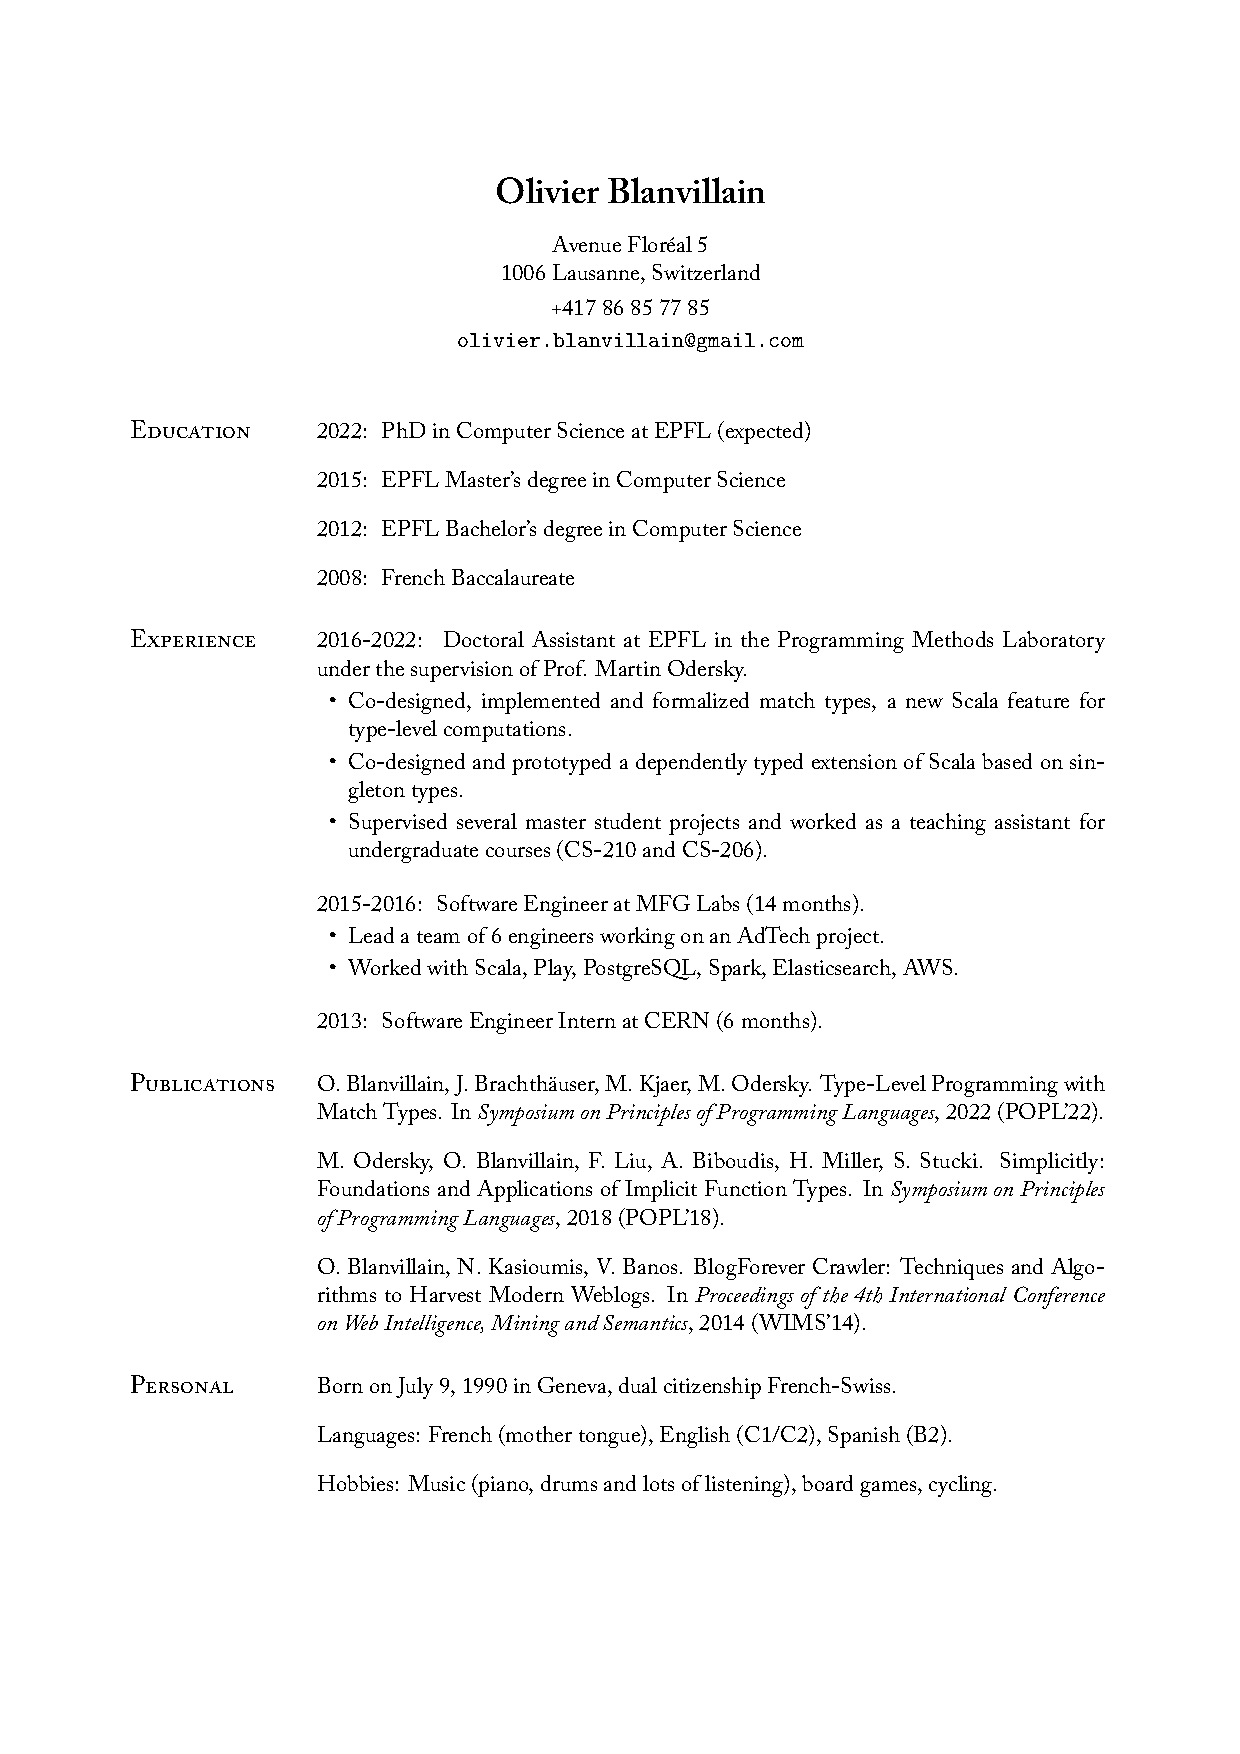
\includepdf{olivier-blanvillain-resume.pdf}
\thispagestyle{empty}~

\end{document}
